\chapter{\texorpdfstring{Searches for new physics in $\tau^+\tau^-$ final states}{Search for new physics in tautau final states}}
\label{sec:bsm_H_to_tau_tau_analysis}
 
The $\tau^+\tau^-$ final states are a powerful tool to search for new physics at collider experiments. 
As the heaviest lepton, $\tau$ particles are sensitive to resonant production of new neutral particles where the couplings have a mass hierarchy.
They are also sensitive to non-resonant effects from new physics mediators. 
This chapter details the searches for two such areas of new physics: additional Higgs bosons and vector leptoquarks.
These searches are split up into three sections: 
\begin{enumerate}[i)]
  \item A model-independent search for a single narrow spin-0 resonance ($\phi$), produced via gluon fusion (gg$\phi$) or in association with a b quark (bb$\phi$). The \ac{SM} Higgs boson is treated as a background and the Yukawa couplings of the spin-0 resonance that contributes to the gluon fusion loop are set to \ac{SM} values.
   \item A search for the \ac{MSSM} Higgs sector in several benchmark scenarios. The benchmark scenarios were proposed in References~\cite{Bahl:2018zmf,Bahl:2020kwe,Bahl:2019ago} and described fully in Reference~\cite{Bagnaschi:2791954}. The $M_{h}^{125}$ and $M_{h,\text{ EFT}}^{125}$ scenarios are shown in this chapter. The production of the observed Higgs boson particle at 125 GeV is also used to constrain the available phase space.
  \item A search for the t-channel exchange of a U(1) vector leptoquark. Two scenarios are taken, motivated by the best fit to the B anomalies as detailed in Section~\ref{sec:b_anomalies}.
\end{enumerate}

These searches are performed with the full Run 2 dataset ($138 \sifb$) collected by the \ac{CMS} experiment. 
The search for additional Higgs bosons had previously been performed with data collected in 2016 ($39 \sifb$) and results were consistent with the \ac{SM} background prediction \cite{CMS_MSSM_Tau_2018}.
 
\section{Signal modelling} 
 
\subsection{Additional Higgs bosons} 
\label{sec:additional_higgs_bosons} 
 
Extended Higgs sectors, such as that of the \ac{MSSM}, can be probed by direct searches for the additional bosons and further precise measurements of the \ac{SM} Higgs boson. 
This search for an extended Higgs sector is motivated by a Type II \ac{2HDM}, such as the \ac{MSSM}.
In these models, $\tan\beta$ enhances couplings of additional Higgs bosons to down-type quarks and charged leptons, whilst up-type quark couplings are suppressed.
This divides the dominant production modes of the Higgs boson into two categories: gluon fusion and production in association with a b quark.
Examples of the Feynman diagrams for these processes are shown in Figure~\ref{fig:mssm_feynamn}, where $\phi$ can represent any of the additional neutral Higgs bosons ($\Ph$, $\PH$ or $\PA$) in these diagrams.\\

\begin{figure}[H]
\centering
\begin{subfigure}[b]{0.3\textwidth}
\begin{tikzpicture}[scale=2]
  \begin{feynman}
    \vertex [label=left:$g$] (a1) at (0,0);
    \vertex [label=left:$g$] (a2) at (0,1);
    \vertex (b1) at (1,0);
    \vertex (b2) at (1,1);
    \vertex (c) at (1.7,0.5);
    \vertex [label=right:$\phi$] (d) at (2.7,0.5);

    \diagram* {
      (a1) -- [gluon] (b1),
      (a2) -- [gluon] (b2),
      (b2) -- [fermion] (b1),
      (c) -- [fermion] (b2),
      (b1) -- [fermion] (c),
      (c) -- [scalar] (d),
    };
  \end{feynman}
\end{tikzpicture}
\caption{}
\end{subfigure}


\begin{subfigure}[b]{0.3\textwidth}
\begin{tikzpicture}[scale=2]
  \begin{feynman}
    \vertex [label=left:$g$] (a1) at (0,0);
    \vertex [label=left:$g$] (a2) at (0,1);
    \vertex (b1) at (1,0);
    \vertex (b2) at (1,0.5);
    \vertex (b3) at (1,1);
    \vertex [label=right:$b$] (c1) at (2,0);
    \vertex [label=right:$\phi$] (c2) at (2,0.5);
    \vertex [label=right:$\bar{b}$] (c3) at (2,1);
    \diagram* {
      (a1) -- [gluon] (b1),
      (a2) -- [gluon] (b3),
      (b3) -- [fermion] (b2),
      (b2) -- [fermion] (b1),
      (c3) -- [fermion] (b3),
      (b1) -- [fermion] (c1),
      (b2) -- [scalar] (c2),
    };
  \end{feynman}
\end{tikzpicture}
\caption{}
\end{subfigure}
\hspace{2cm}
\begin{subfigure}[b]{0.3\textwidth}
\begin{tikzpicture}[scale=2]
  \begin{feynman}
    \vertex [label=left:$g$] (a1) at (0,0);
    \vertex [label=left:$b$] (a2) at (0,1);
    \vertex (b) at (0.7,0.5);
    \vertex (c) at (1.4,0.5);
    \vertex [label=right:$b$] (d1) at (2.1,0);
    \vertex [label=right:$\phi$] (d2) at (2.1,1);
    \diagram* {
      (a1) -- [gluon] (b),
      (a2) -- [fermion] (b),
      (b) -- [fermion] (c),
      (c) -- [fermion] (d1),
      (c) -- [scalar] (d2),
    };
  \end{feynman}
\end{tikzpicture}
\caption{}
\end{subfigure}
\vspace*{10mm}
\caption[Feynman diagrams for gluon fusion and production in association with b quarks.]{Diagram (a) shows the production of neutral Higgs bosons from gluon fusion. The dominant loop contributions to these diagrams are from t-only, b-only and tb-interference. Diagrams (b) and (c) show production in association with b quarks.}
\label{fig:mssm_feynamn}
\end{figure}

With the $\tan\beta$ enhancement, the decays of additional Higgs bosons to $\tau$ leptons and b quarks are most dominant.
$\tau$ leptons are identified with higher purity than b quarks at the \ac{CMS} detector.
It is also easier to separate $\tau^{+}\tau^{-}$ from the large \ac{QCD} multijet background produced from the high-energy proton-proton collisions.
This was confirmed with the 2016 dataset and although no deviations were observed, the strongest limits on the \ac{MSSM} phase space were placed by the $\tau^+\tau^-$ final states \cite{CMS_MSSM_Tau_2018,CMS:2018hir}. \\

For this analysis, signal templates for the production of additional Higgs bosons over a mass range of 60 GeV to 3.5 TeV are generated.
Gluon fusion is simulated at \ac{NLO} precision using the \ac{2HDM} implementation of \POWHEG 2.0~\cite{Nason:2004rx,Frixione:2007vw,Alioli:2010xd,Jezo:2015aia}.
The kinematic properties are highly dependent on the contributions to the loop, and these are dependent on the specific signal model.
To account for the t quark only, b quark only, and tb-interference loop contributions at the \ac{NLO} plus parton shower prediction, weights are calculated from the $\pT$ spectra to split these contributions up.
Once individual templates have been determined for each contribution to the loop, the \ac{2HDM} samples can be scaled to the \ac{MSSM} scenario prediction with the following formula,

\begin{align}
& \frac{d\sigma_{\text{MSSM}}}{d\pT}  = \left(\frac{Y_{t,\text{MSSM}}}{Y_{t,\text{2HDM}}}\right)^{2}\frac{d\sigma^{t}_{\text{2HDM}}}{d\pT}(Q_{t}) + \left(\frac{Y_{b,\text{MSSM}}}{Y_{b,\text{2HDM}}}\right)^{2}\frac{d\sigma^{b}_{\text{2HDM}}}{d\pT}(Q_{b}) \nonumber \\
& + \left(\frac{Y_{t,\text{MSSM}}}{Y_{t,\text{2HDM}}}\frac{Y_{b,\text{MSSM}}}{Y_{b,\text{2HDM}}}\right) \left\{ \frac{d\sigma^{t+b}_{\text{2HDM}}}{d\pT}(Q_{tb}) - \frac{d\sigma^{t}_{\text{2HDM}}}{d\pT}(Q_{tb}) - \frac{d\sigma^{b}_{\text{2HDM}}}{d\pT}(Q_{tb}) \right\} ,
\label{eqn:mssm_xs}
\end{align}
\vspace{0.2cm}

where $Q_i$ are resummation scales that depend on the mass of the additional Higgs boson, and $\sigma^{i}_{j}$ and $Y^{i}_{j}$ are the determined cross-sections and Yukawa couplings of the relevant theory $j$ and contribution $i$.
Further contributions from any supersymmetric partners were checked and accounted for less than a few percent and so are neglected.
The $\pT$ reweighting is done separately for the scalar and pseudoscalar additional Higgs bosons, as the $\pT$ distributions can differ.
The benchmark scenarios provide the relative Yukawa couplings (to calculate the cross-sections) and branching fractions of the \ac{MSSM} Higgs bosons.
An example of the distributions for gluon fusion production, in the \ac{MSSM} $M_{h}^{125}$ scenario with $m_{A} = 500$ GeV whilst varying $\tan\beta$, is shown in Figure~\ref{fig:mssm_sig}.
The distributions peak at a higher $\pT$ for the t quark loop, therefore at smaller $\tan\beta$, where the t quark contribution is dominant, an additional Higgs boson would be more boosted. \\

\begin{figure}[!hbtp]
\centering
    \subfloat[]{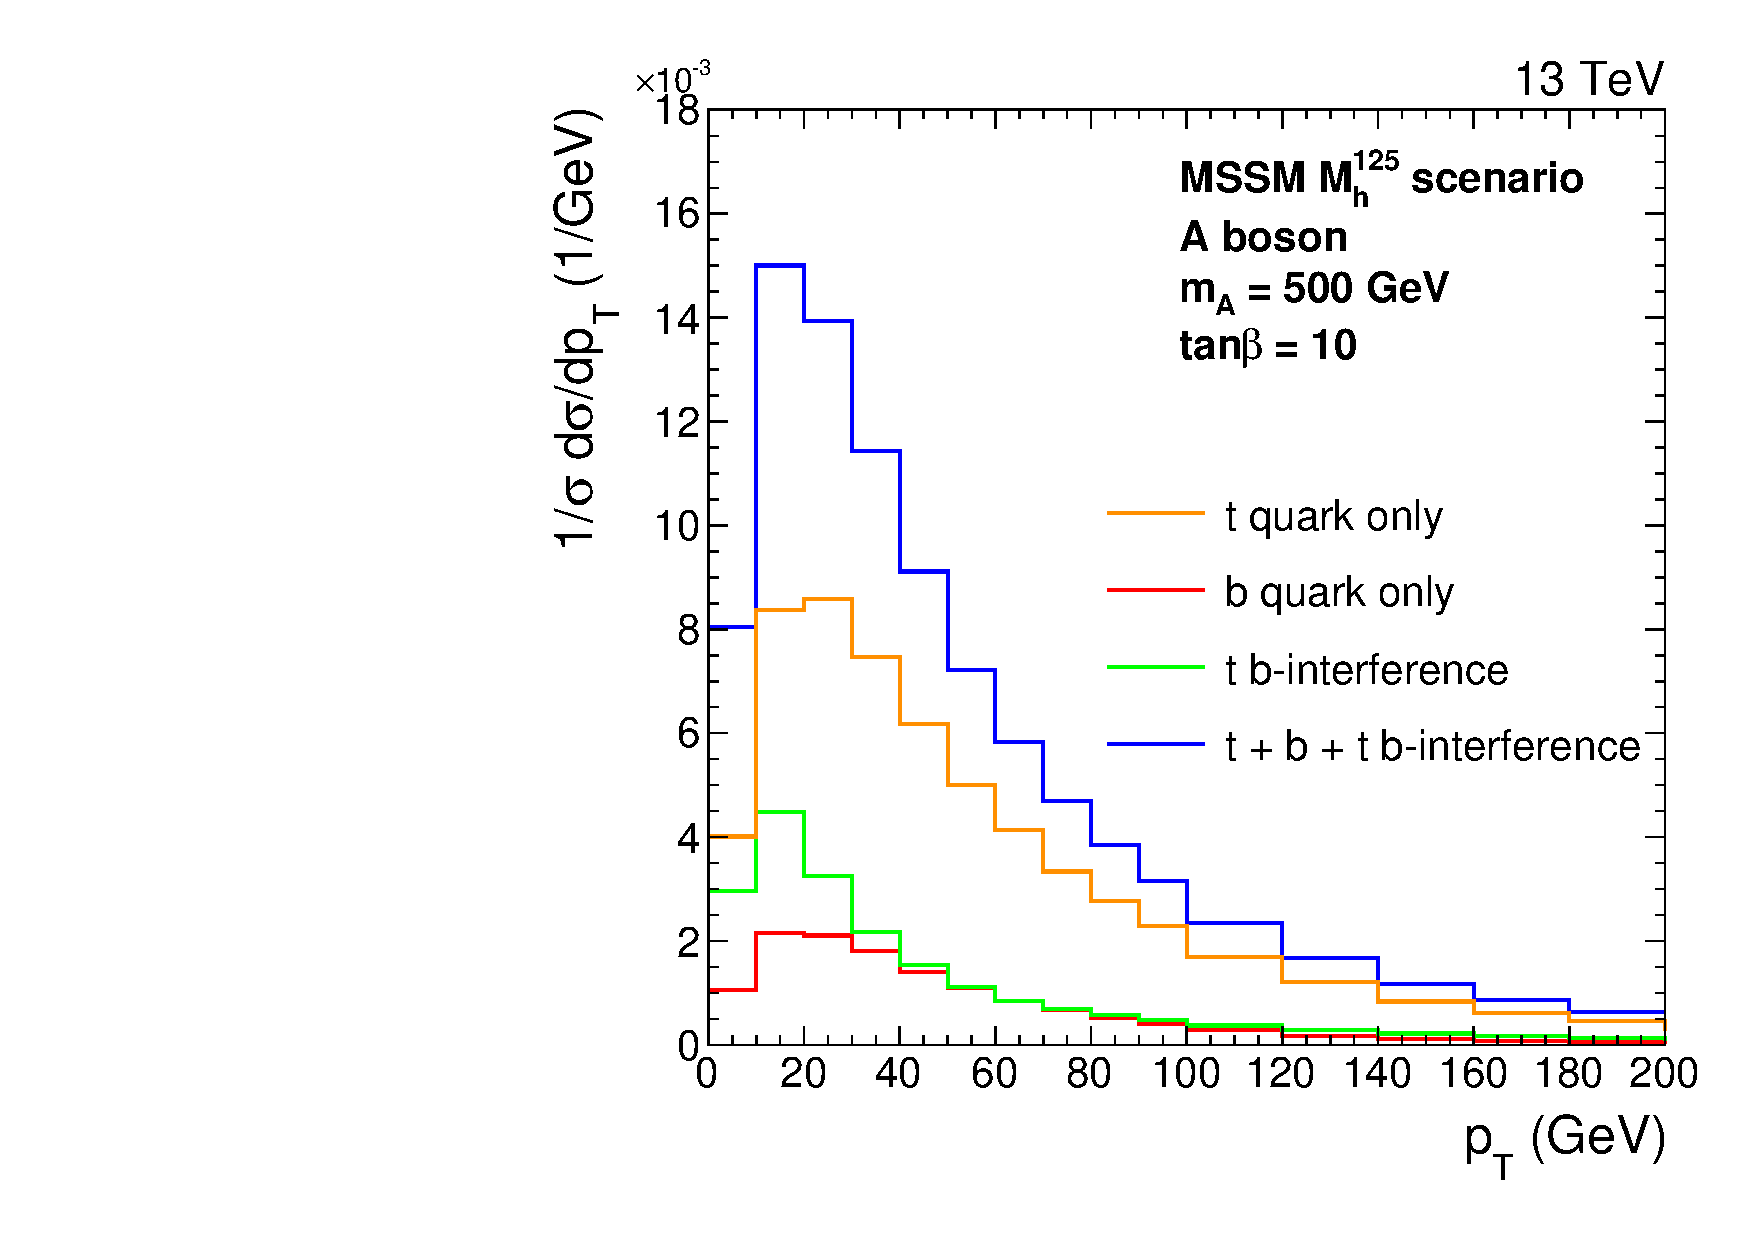
\includegraphics[width=0.5\textwidth]{Figures/pT_reweighting_plot_A10.pdf}}
    \subfloat[]{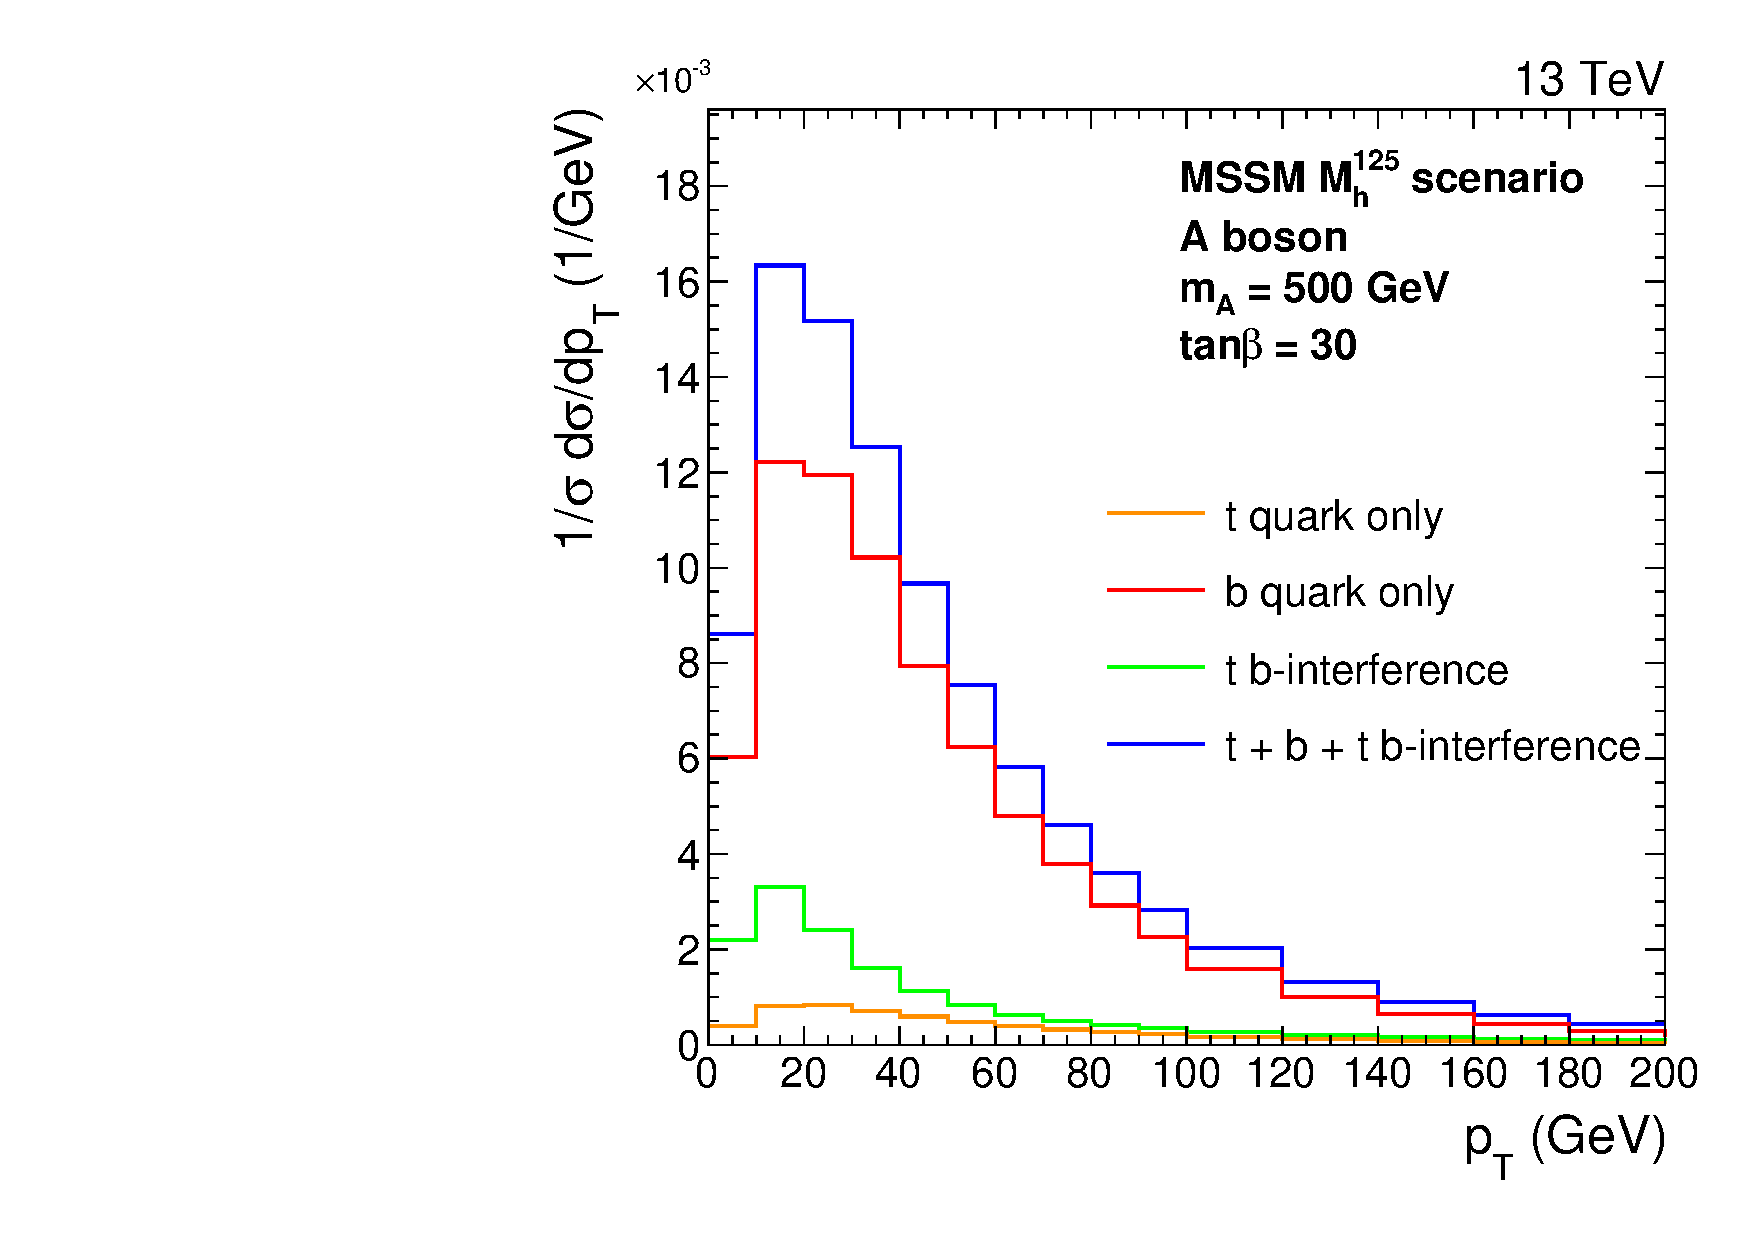
\includegraphics[width=0.5\textwidth]{Figures/pT_reweighting_plot_A30.pdf}} \\
    \subfloat[]{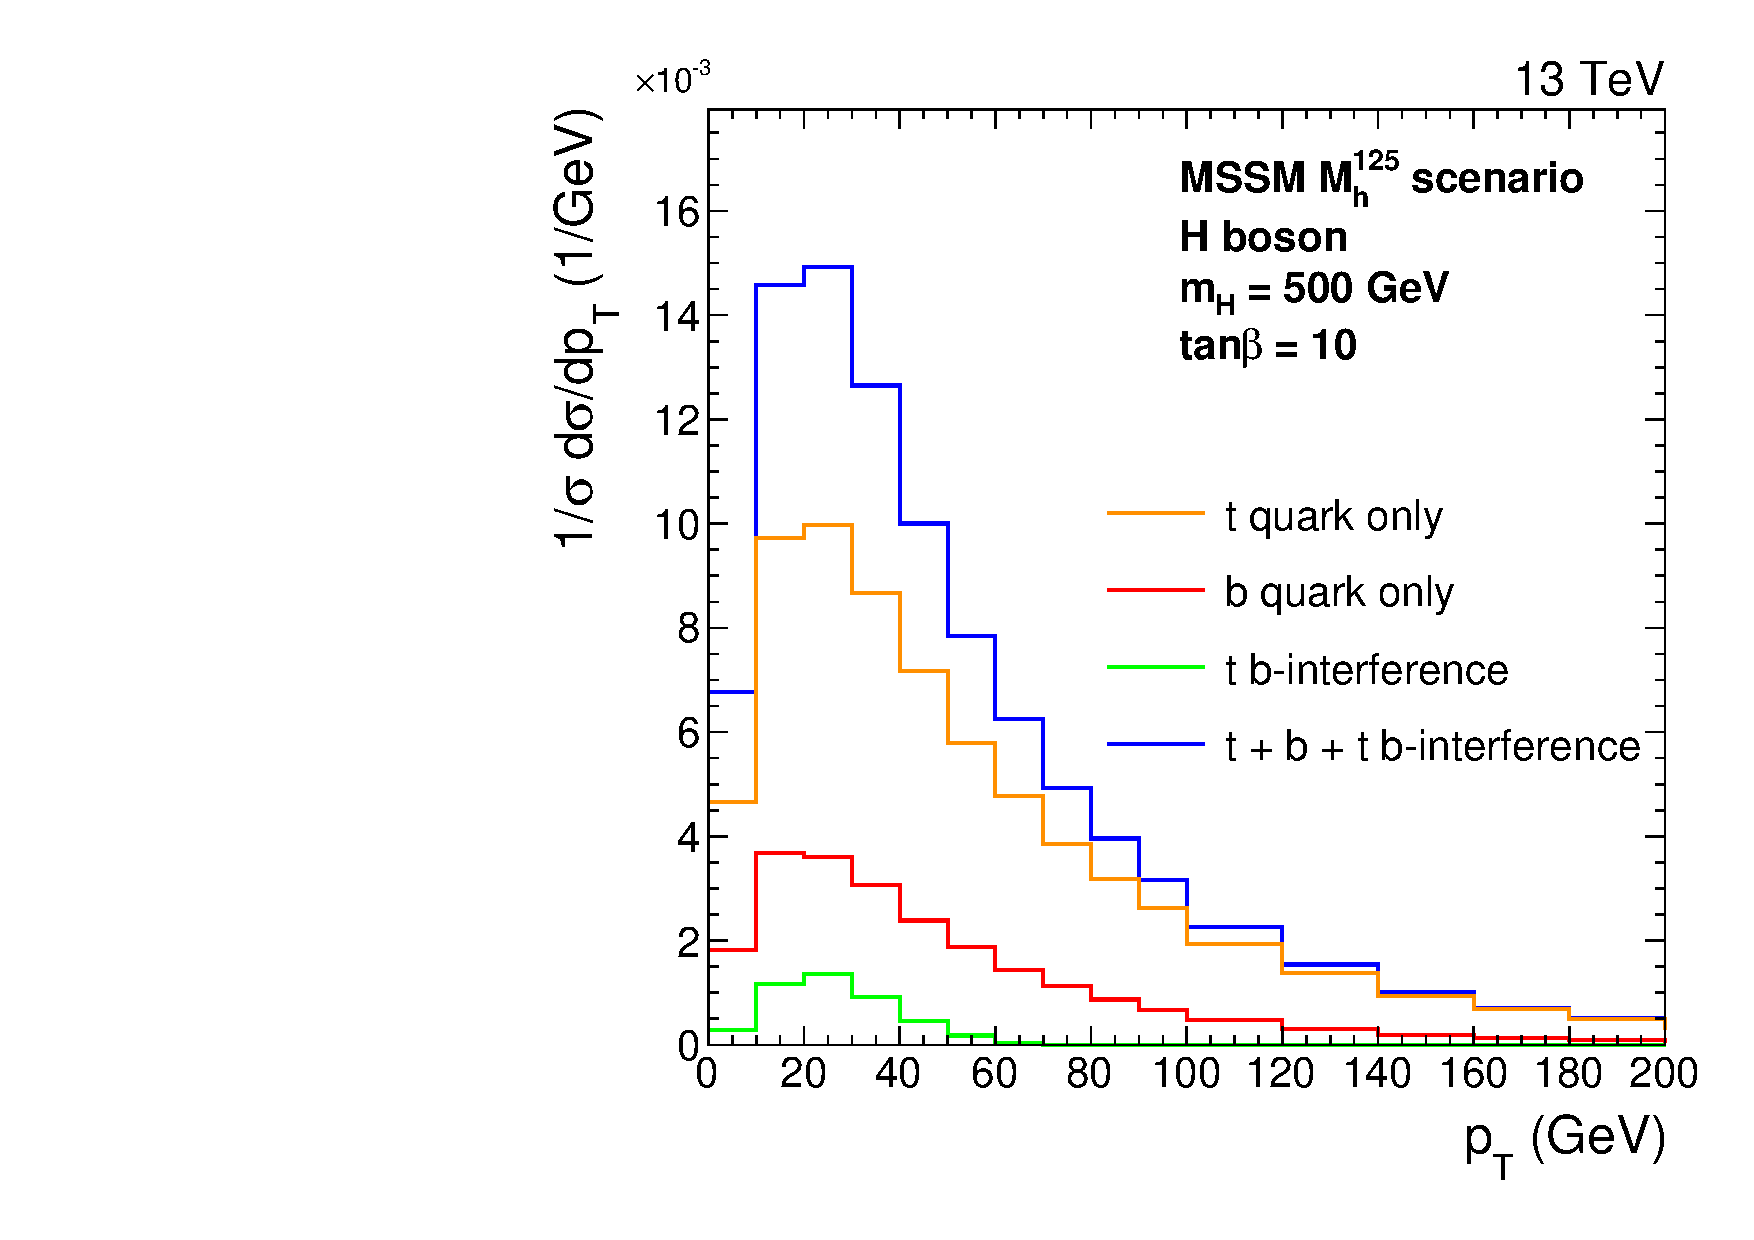
\includegraphics[width=0.5\textwidth]{Figures/pT_reweighting_plot_H10.pdf}}
    \subfloat[]{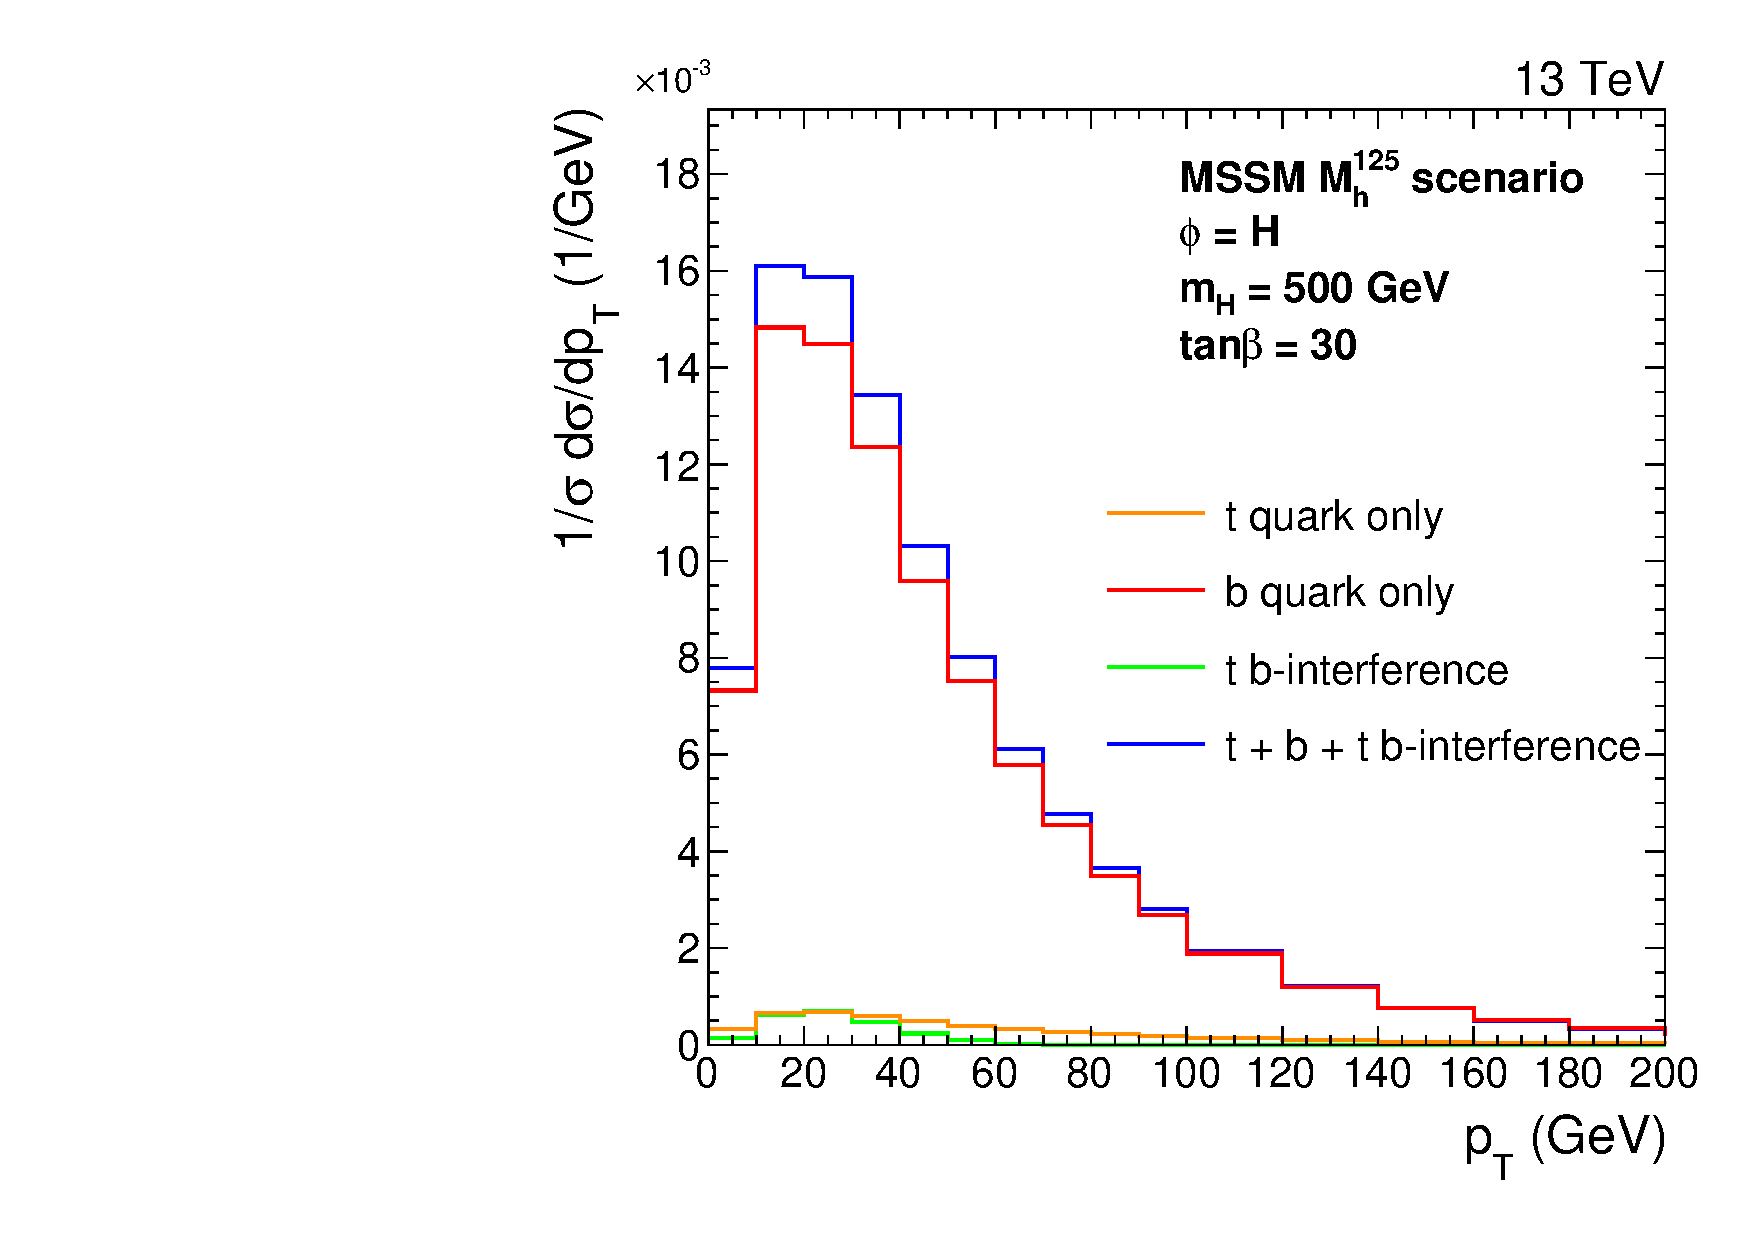
\includegraphics[width=0.5\textwidth]{Figures/pT_reweighting_plot_H30.pdf}} \\
\caption[Plots of the gluon fusion generator level $\pT$ distributions, when changing the MSSM parameters.]{$p_{T}$ density distributions of the A (top) and H (bottom) boson, with contributions to the gluon fusion loop displayed individually and summed. These are shown for $\tan\beta$ values of 10 (left) and 30 (right) where $m_{A} = 500$ GeV in the MSSM $M_{h}^{125}$ scenario.}
\label{fig:mssm_sig}
\end{figure}

Production in association with b quarks is simulated at \ac{NLO} precision using the corresponding \POWHEG 2.0 implementation in the four \ac{FS}~\cite{Nason:2004rx,Frixione:2007vw,Alioli:2010xd,Jezo:2015aia}.
All additional Higgs boson signal generation is performed using the parton distribution function NNPDF3.1~\cite{Ball:2014uwa,Ball:2017nwa}.
$\tau$ lepton decay, parton showering and hadronisation are all modelled with the \PYTHIA event generator where the \ac{PU} profile is matched to data~\cite{Sirunyan:2019dfx,Sjostrand:2014zea}.
All events generated are passed through a \texttt{GEANT4}-based \cite{Agostinelli:2002hh} simulation of the \ac{CMS} detector and reconstructed in the same way as data. \\

The model-independent and model-dependent additional neutral Higgs boson searches explained in this chapter, utilise the same signal templates generated. 
The differences lie in the scaling of the gluon fusion cross-section and loop contributions (set to the Yukawa couplings for the model-independent interpretation), and the b associated production cross-section, as well as taking into account the branching fractions in the model-dependent interpretation.
The model-dependent search for the \ac{MSSM} also looks to find differences between the observed \ac{SM} Higgs boson and the predicted \ac{MSSM} \ac{SM}-like Higgs boson.
In each \ac{MSSM} benchmark scenario, an uncertainty of $\pm 3$ GeV is given on the prediction for the \ac{SM} Higgs boson mass.
This uncertainty is to reflect the contribution of any unknown higher-order corrections.
The value of the mass is allowed to vary within this window, however, the Yukawa couplings are rescaled to that of the observed mass.

\subsection{Vector leptoquarks}
\label{sec:vlq}

The best fit to the B anomalies in the available phase space for vector leptoquarks yielded a large b quark and $\tau$ lepton coupling to the U(1) particle.
The possible production modes of a $\tau^+\tau^-$ final state are shown in Figure~\ref{fig:leptoquark_feynman}. \\

\begin{figure}[t]
\centering
\begin{subfigure}[b]{0.3\textwidth}
\begin{tikzpicture}[scale=2]
  \begin{feynman}
    \vertex [label=left:$\bar{q}$] (a1) at (0,0);
    \vertex [label=left:$q$] (a2) at (0,1);
    \vertex (b1) at (1,0);
    \vertex (b2) at (1,1);
    \vertex [label=right:$U_{1}$] (b3) at (1,0.5);
    \vertex [label=right:$\tau^-$] (c1) at (2,0);
    \vertex [label=right:$\tau^+$] (c2) at (2,1);

    \diagram* {
      (b1) -- [fermion] (a1),
      (a2) -- [fermion] (b2),
      (b2) -- [boson] (b1),
      (c1) -- [fermion] (b1),
      (b2) -- [fermion] (c2),
    };
  \end{feynman}
\end{tikzpicture}
\caption{}
\end{subfigure} \\

\begin{subfigure}[b]{0.3\textwidth}
\begin{tikzpicture}[scale=2]
  \begin{feynman}
    \vertex [label=left:$g$] (a1) at (0,0);
    \vertex [label=left:$g$] (a2) at (0,1);
    \vertex (b1) at (0.7,0.5);
    \vertex (b2) at (1.2,0.5);
    \vertex (c1) at (1.7,0.1);
    \vertex (c2) at (1.7,0.9);
    \vertex [label=$U_{1}$] (c1t) at (1.4,-0.05);
    \vertex [label=$U_{1}$] (c2t) at (1.4,0.72);
    \vertex [label=right:$\tau^+$] (d1) at (2.2,1.2);
    \vertex [label=right:$q$] (d2) at (2.2,0.6);
    \vertex [label=right:$\tau^-$] (d3) at (2.2,0.4);
    \vertex [label=right:$\bar{q}$] (d4) at (2.2,-0.2);
    
    \diagram* {
      (a1) -- [gluon] (b1),
      (a2) -- [gluon] (b1),
      (b1) -- [gluon] (b2),
      (b2) -- [scalar] (c1),
      (b2) -- [scalar] (c2),
      (d1) -- [fermion] (c2),
      (c2) -- [fermion] (d2),
      (c1) -- [fermion] (d3),
      (d4) -- [fermion] (c1),
    };
  \end{feynman}
\end{tikzpicture}
\caption{}
\end{subfigure}
\hspace{2cm}
\begin{subfigure}[b]{0.3\textwidth}
\begin{tikzpicture}[scale=2]
  \begin{feynman}
    \vertex [label=left:$g$] (a1) at (0,0);
    \vertex [label=left:$q$] (a2) at (0,1);
    \vertex (b1) at (0.7,0.5);
    \vertex [label=below:$q$] (bt) at (0.95,0.45);
    \vertex (b2) at (1.2,0.5);
    \vertex [label=right:$\tau^-$] (c1) at (2,0);
    \vertex (c2) at (1.7,0.9);
    \vertex [label=$U_{1}$] (c2t) at (1.4,0.72);
    \vertex [label=right:$\tau^+$] (d1) at (2.2,1.2);
    \vertex [label=right:$q$] (d2) at (2.2,0.6);

   
    \diagram* {
      (a1) -- [gluon] (b1),
      (a2) -- [fermion] (b1),
      (b1) -- [fermion] (b2),
      (b2) -- [fermion] (c1),
      (b2) -- [scalar] (c2),
      (d1) -- [fermion] (c2),
      (c2) -- [fermion] (d2),
    };
  \end{feynman}
\end{tikzpicture}
\caption{}
\end{subfigure}
\vspace*{10mm}
\caption[Feynman diagrams for the production of a di-$\tau$ final state from vector leptoquarks.]{Feynman diagrams showing the contribution from U(1) vector leptoquarks to the final state with a pair of oppositely charged $\tau$ leptons. $q$ represents any SM quark. The t-channel (a), pair (b) and single (c) productions of a vector leptoquark are shown.}
\label{fig:leptoquark_feynman}
\end{figure}

Pair and single production of a vector leptoquark are dependent on its strong coupling, which is highly model dependent.
For large mass, $m_U$, the probability of producing an on-shell U(1) singlet or pair is heavily suppressed due to the momentum of the initial partons.
These production processes are not discussed further in this chapter.
A search for single and pair production at the \ac{CMS} experiment was performed and no statistically significant deviation was observed~\cite{CMS:2022zks}.
Single production places the loosest constraints on the available phase space, out of the processes mentioned.
Pair production puts a lower limit on the leptoquark mass, as the process is approximately independent of $g_U$. 
However, this limit is heavily dependent on the value chosen for the strong coupling. \\

The t-channel process contains two vertices with a U(1) vector leptoquark, a quark and a $\tau$ lepton, and hence the cross-section will scale with $g_{U}^4$ ($g_{U}^2$ for each vertex).
From the best fit to B anomalies, the vertex is dominated by the b quark and hence the initial state will be mostly from $b\bar{b}$, with sub-dominant contributions from $b\bar{s}$, $s\bar{b}$ and $s\bar{s}$.
Although there are no additional b quarks in the final state in the \ac{LO} process, the production of initial state b quarks can lead to additional b quarks in the final state.
In this search, the two scenarios discussed in Section~\ref{sec:b_anomalies} are considered.
The only non-negligible freely floating parameter in each fit, for $\tau^{+}\tau^{-}$ final states in the $m_{U}$-$g_{U}$ phase space is the $\beta_{L}^{s\tau}$ parameter.
This is set to the best-fit value. \\

The signal process of a t-channel exchange is simulated in the five \ac{FS} at \ac{LO} precision using the \MGvATNLO v2.6.5 event generator~\cite{Alwall:2011uj}.
Events are generated with one or fewer outgoing partons from the matrix element and the MLM prescription~\cite{Frederix:2012ps} is then used for matching, with a scale set to 40 GeV.
Negligible dependence of the decay width is observed. 
For simulation, this is chosen to approximately match the value predicted by the B anomaly fit~\cite{Cornella:2021sby}.
Samples with a mass between 1 and 5 TeV are generated. \\

The interference between the signal and $Z/\gamma^* \rightarrow \tau\tau$ process was checked and a large destructive effect was observed, with magnitude dependent on $g_{U}$.
To account for this, separate samples are produced for this interference, using the same generators as the t-channel exchange.
The interference samples are generated with extra statistics at large di-$\tau$ mass values, to have a sufficient number of events in the regions of interest for the signal.
The cross-section of these interference samples scales with $g_{U}^2$. 
Examples of the generator level di-$\tau$ mass distributions are shown in Figure~\ref{fig:vlq_signal}. \\

\begin{figure}[!hbtp]
\centering
    \subfloat[]{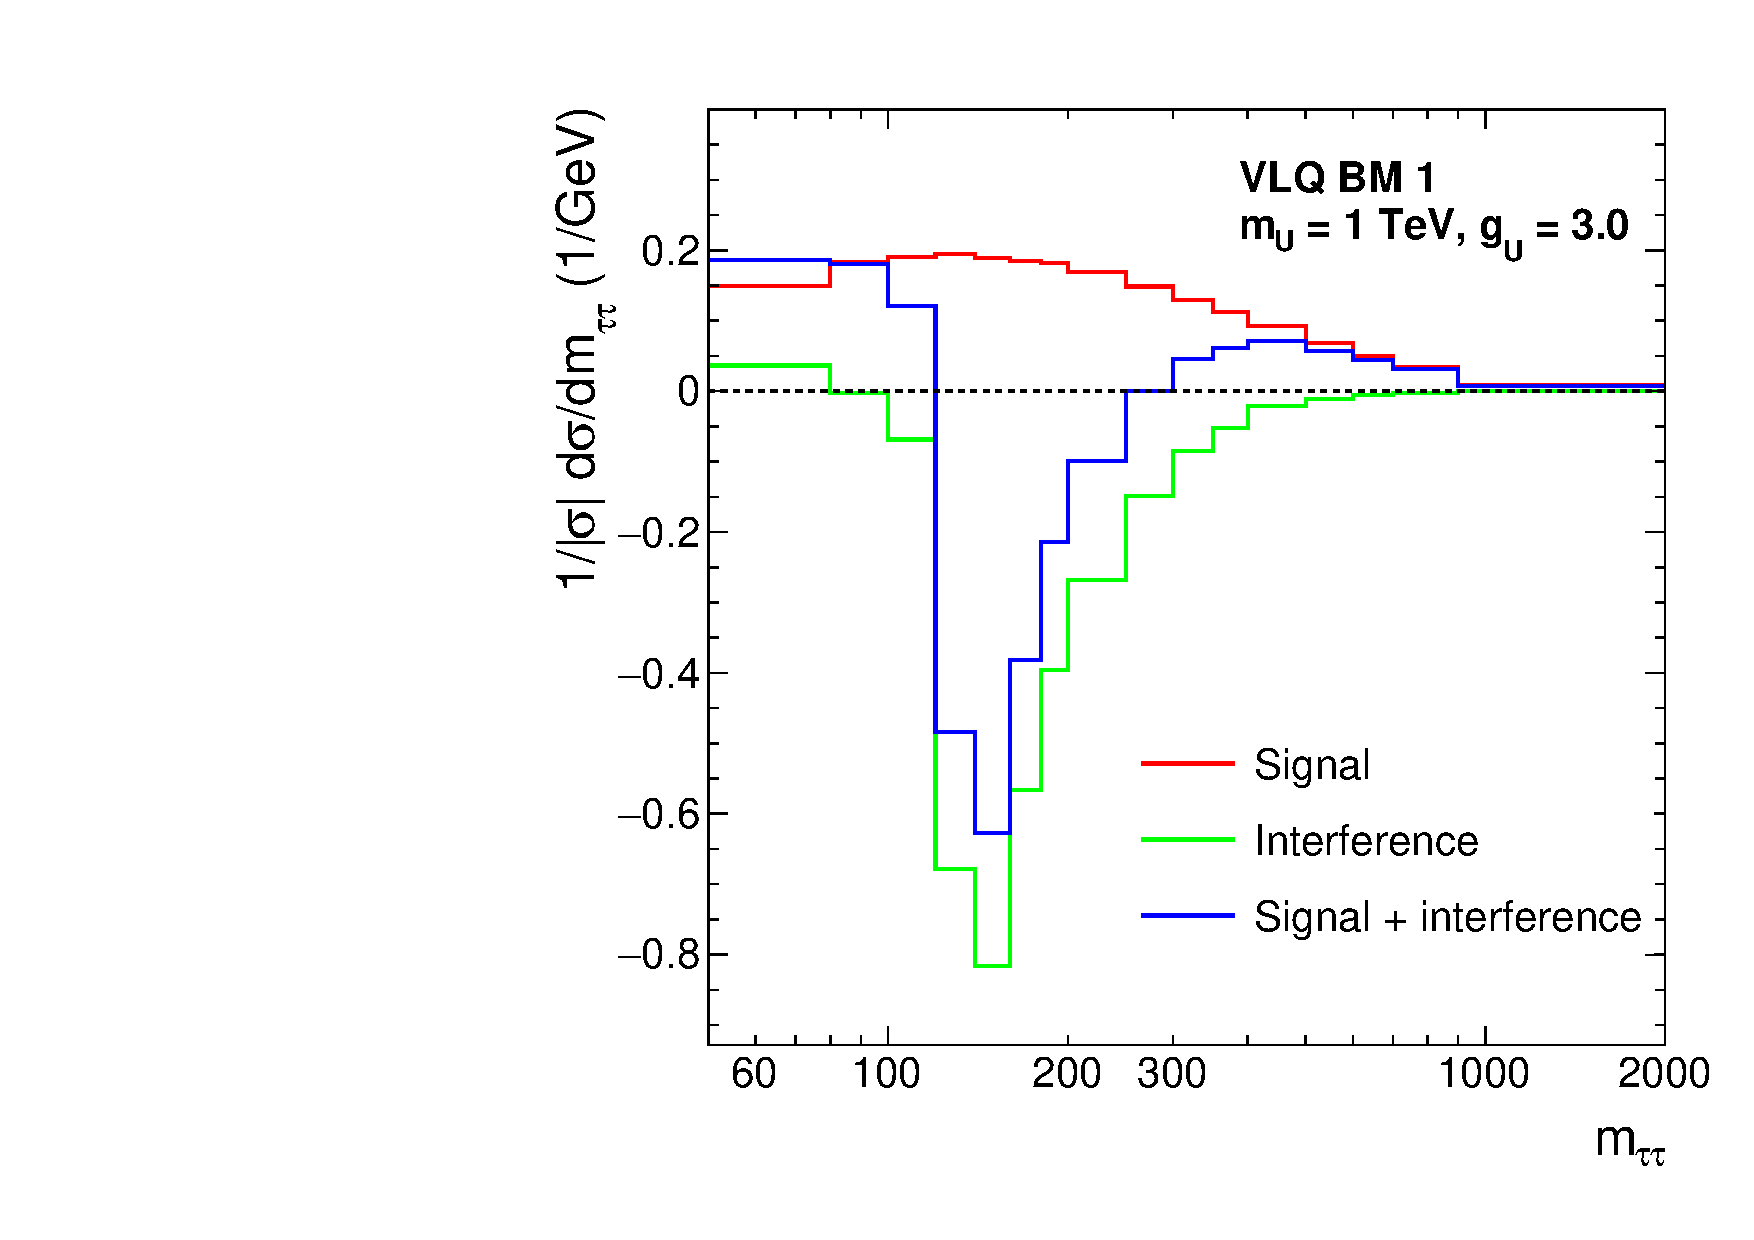
\includegraphics[width=0.5\textwidth]{Figures/vlq_signal_plot_gU3.pdf}}
    \subfloat[]{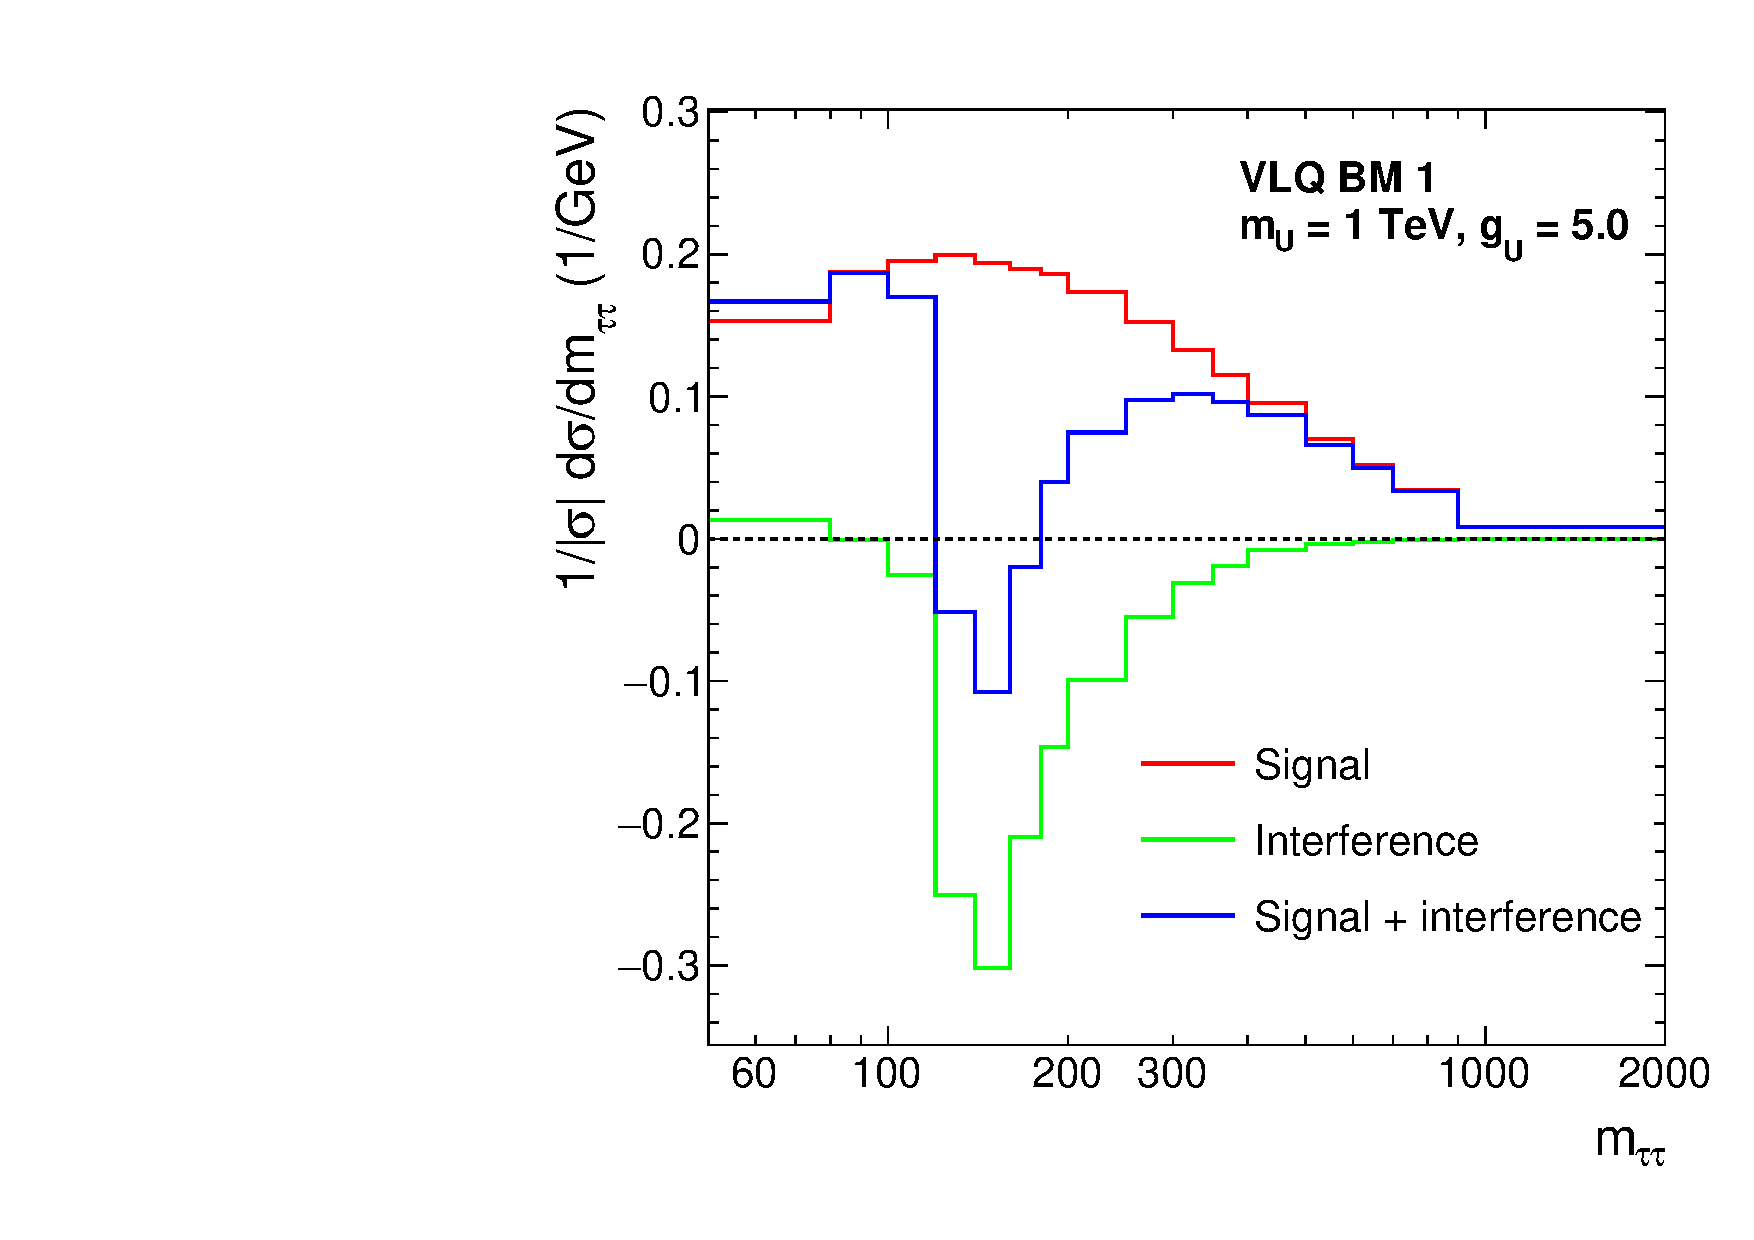
\includegraphics[width=0.5\textwidth]{Figures/vlq_signal_plot_gU5.pdf}}
\caption[Plots of the vector leptoquark generator level $m_{\tau\tau}$ distributions, when changing $g_{U}$.]{The generator level $m_{\tau\tau}$ density distributions of the t-channel vector leptoquark signal and the interference with $Z/\gamma^* \rightarrow \tau\tau$. This is shown in the VLQ BM 1 scenario for a leptoquark of mass 1 TeV for coupling strengths of $g_{U}=3$ (a) and $g_{U}=5$ (b).}
\label{fig:vlq_signal}
\end{figure}

The t-channel signal produces a broad distribution in $m_{\tau\tau}$ due to its non-resonant nature.
The interference is mostly a destructive effect (except for at small $m_{\tau\tau}$), with the yield becoming less negative at higher $m_{\tau\tau}$.
The interference peaks negatively between 100 and 200 GeV and in this region, the combined yield can be negative.
This negative signal yield would diminish the $Z/\gamma^{*}$ background.
Due to the difference in the scaling of the two effects, at small $g_{U}$ the interference is more dominant than the signal and hence the yield of the combined result is reduced.

\section{Event selection}

The possible decays of two $\tau$ leptons and their branching fractions, where the $\tau$ decay is grouped into three categories; $e$, $\mu$ and $\tau_h$ as defined in Section~\ref{sec:object_reconstruction}, are shown in Table~\ref{tab:ditau_br}. 
For this search, the four largest branching fraction channels are used: $\tauhtauh$, $\etauh$, $\mutauh$ and $e\mu$.
This accounts for approximately 94\% of di-$\tau$ events.
The two same lepton channels are neglected due to the small branching ratio and the dominating $Z\rightarrow ee$ and $Z\rightarrow \mu\mu$ backgrounds. \\

\begin{table}[!hbtp]
    \centering
    \begin{tabular}{|c|c|}
         \hline
         Channel & Branching Fraction  \\
         \hline
         \hline
         $\tauhtauh$ & 42.0\% \\
         $\etauh$ & 23.1\% \\
         $\mutauh$ & 22.6\% \\
         $\emu$ & 6.2\% \\
         $e e$ & 3.2\% \\
         $\mu \mu$ & 3.0\% \\
         \hline
    \end{tabular}
    \caption[Branching fractions of the decays of two $\tau$ leptons.]{Branching fractions of the decays of two $\tau$ leptons.}
    \label{tab:ditau_br}
\end{table}

\subsection{Trigger requirements}
\label{sec:trig_ditau}

In these four final state pairs, several different online trigger requirements are needed.
In the $\tauhtauh$ channel, two possible triggers are available: the double-$\tauh$ and single-$\tauh$ triggers.
The single-$\tauh$ trigger has a high $\pT$ threshold at 120 (180) GeV for events recorded in 2016 (2017-2018), whilst the double-$\tauh$ trigger has a $\pT$ threshold at 40 GeV.
Therefore, the double-$\tauh$ trigger is used unaccompanied when the $\tauh$ has $\pT$ below the single-$\tauh$ threshold and the union of single-$\tauh$ and double-$\tauh$ triggered events are taken above the threshold. \\

In the $\etauh$ and $\mutauh$ channels, there are three possible triggers available: the single-e/$\mu$, single-$\tauh$ and the e/$\mu$-$\tauh$ cross-trigger.
The $\pT$ thresholds of the light lepton leg of these triggers are shown in Table~\ref{tab:trig_thresholds}.
The cross-trigger is used for events where the light lepton has $\pT$ between the thresholds for the cross-trigger and single-$e/\mu$ trigger.
The light lepton used in the cross-trigger is required to be in the central barrel of the detector within $|\eta| < 2.1$, and the $\tauh$ triggered on is required to have $\pT >$ 30 GeV.
Above these light lepton cross-trigger $\pT$ thresholds, the single-$e/\mu$ trigger is used.
At $\tauh$ $\pT$ above the single-$\tauh$ thresholds, the single-$\tauh$ trigger is used in combination with the single-$e/\mu$ trigger. \\

\begin{table}[hbtp]
  \centering
  \begin{tabular}{|c||c|c|c|c|}
    \hline
    Year/ Trigger   & e-$\tauh$ cross-trigger & single-$e$ & $\mu$-$\tauh$ cross-trigger & single-$\mu$ \\
    \hline
    \hline
    2016 & 23                    & 26         & 20                     & 23           \\
    2017 & 25                    & 28         & 20                     & 25           \\
    2018 & 25                    & 33         & 21                     & 25           \\
    \hline        
  \end{tabular}
  \caption[Trigger $\pT$ thresholds of light lepton triggers.]{Lower trigger $\pT$ thresholds in GeV on light leptons for the $\etauh$ and $\mutauh$ channels.}
  \label{tab:trig_thresholds}  
\end{table}

In the $\emu$ channel, there are three possible triggers available: the single-$e$, single-$\mu$ and the e-$\mu$ cross-trigger.
However, only the cross-trigger is used in this analysis, due to the larger efficiencies of correctly selecting light leptons.
The electron and muon are required to have $\pT >$ 15 GeV and $|\eta| < 2.4$.

\subsection{Offline requirements}

All offline selections stated are in addition to the object selection discussed in Chapter~\ref{sec:object_reconstruction}.
In this analysis, $\tau_h$ candidates are required to pass the \texttt{DeepTau} \texttt{Medium} $D_{\text{jet}}^{\text{WP}}$, as described in Section~\ref{sec:taus}.
The $D_{e}^{\text{WP}}$ and $D_{\mu}^{\text{WP}}$ choices are dependent on the decay channel.
The \texttt{VVLoose}, \texttt{Tight}, \texttt{VVLoose} $D_{e}^{\text{WP}}$ and the \texttt{VLoose}, \texttt{VLoose} and \texttt{Tight} $D_{\mu}^{\text{WP}}$ are used in the $\tauhtauh$, $\etauh$ and $\mutauh$ channels respectively.
The tighter working point for the same light lepton discrimination as tagged in the event is used to remove light leptons misidentified as a $\tau_h$ candidate from the $Z \rightarrow \ell\ell$ process.
The light lepton isolation requirement is $\Irel < 0.15$ for both electrons and muons, except for in the $\emu$ channel where the muon is required to have $\Irel < 0.2$. \\

The selected $\tau$ lepton decay candidates are required to have opposite charges and to be separated by more than $\Delta R$ > 0.5 in all channels except $\emu$ where $\Delta R$ > 0.3 is required.
In events where the number of an object is greater than the required number of objects for the decay channel, the objects are sorted and the leading objects are chosen.
This is done by the maximum $D_{\text{jet}}^{\text{score}}$ if a $\tau_h$ candidate, or minimum $\Irel$ if a light lepton candidate.
To maintain orthogonality between channels, events with additional light leptons passing looser selections than the nominal requirements, are rejected from the selection.
The looser selections vetoed, help to suppress the $Z \rightarrow \ell\ell$ background process further, as well as keeping the channels orthogonal. \\

In the $\etauh$ and $\mutauh$ channels, a cut is placed on the transverse mass between the light lepton $\pTvec$ and the missing $\pTvec$ at 70 GeV, where the transverse momentum is defined as,
\begin{equation}
m_{\text{T}}(\pTvec^{\hspace{2pt}i},\pTvec^{\hspace{2pt}j}) = \sqrt{2\pT^{i}\pT^{j}(1-\cos\Delta\phi)},
\label{eqn:mt}
\end{equation}
where $\Delta\phi$ to the azimuthal angle between $\pTvec^{\hspace{2pt}i}$ and $\pTvec^{\hspace{2pt}j}$.
The variable is used to remove W + jets background events, where a jet is misidentified as a $\tau_h$.
In these events, the \ac{MET} (neutrino) and light lepton from the W decay are aligned and hence the event has a large $m_{T}(\pTvec^{\hspace{2pt}e/\mu},\pTvec^{\hspace{2pt}\text{miss}})$. \\

In the $\emu$ channel, an additional cut is placed on the variable $D_{\zeta}$, which is defined as,
\begin{equation}
D_\zeta = p_\zeta^\text{miss} - 0.85 p_\zeta^\text{vis};\qquad
p_\zeta^\text{miss} = \pTvec^{\hspace{2pt}\text{miss}} \cdot \hat{\zeta};\qquad
p_\zeta^\text{vis} = (\pTvec^{\hspace{2pt}e} + \pTvec^{\hspace{2pt}\mu}) \cdot \hat{\zeta}
\label{eqn:Dzeta_def}
\end{equation}
where $\hat{\zeta}$ is the bisectional direction between the electron and the muon in the transverse plane.
A diagram of the inputs is shown in Figure~\ref{fig:dzeta_diagram}. \\
\begin{figure}[!hbtp]
\centering
    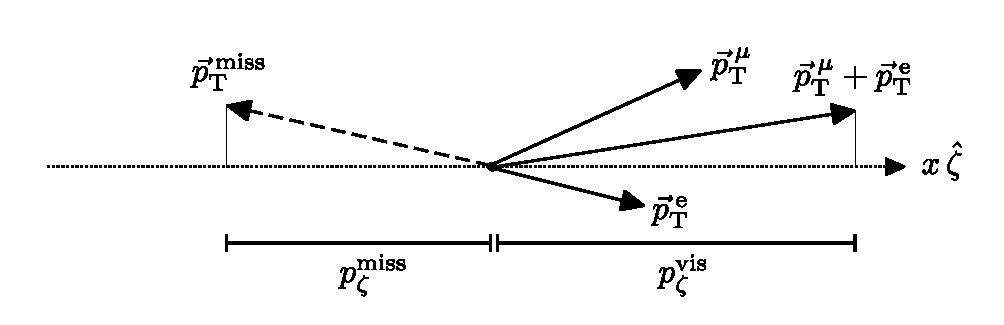
\includegraphics[width=1.0\textwidth]{Figures/dzeta_diagram.pdf}
\caption[Diagram of the inputs to the $D_\zeta$ variable.]{Diagram of the inputs to the $D_\zeta$ variable~\cite{CMS:2022rbd}.}
\label{fig:dzeta_diagram}
\end{figure}

The linear combination is optimised for genuine di-$\tau$ events to peak around $D_{\zeta} = 0$ GeV. 
It is motivated by the expectation that in di-$\tau$ decays from a resonance, the visible and missing (from $\tau$ neutrinos) momenta are roughly aligned and of similar magnitudes.
In W + jets and $\ttbar$ events, the directions of the visible and missing products are expected to be more randomly distributed and lead to a non-peaking $D_{\zeta}$.
Therefore, only events with $D_\zeta >$ -35 GeV are considered for signal events.
No b tag events failing this cut are vetoed, and events with a b tag also failing this cut are used for a $\ttbar$ control region.

\section{Search optimisation}
\label{sec:search_optimisation}

The optimisation of the signal extraction depends on which of the three scenarios, set out at the beginning of this section, is being searched for.
The components of the optimisation are named the high-mass, low-mass and \ac{SM} Higgs optimisation procedures.
For the model-independent search (i) the high- or low-mass optimisation procedures are used depending on whether the mass of the resonance is greater or less than 250 GeV.
The search for the \ac{MSSM} Higgs sector (ii) uses the high mass or the \ac{SM} Higgs optimisation procedures depending on whether the reconstructed di-$\tau$ mass is greater or less than 250 GeV.
The presence of more than one neutrino in the event means that it is not possible to fully reconstruct the di-$\tau$ mass directly.
Instead, the likelihood-based \texttt{SVFit} algorithm is used \cite{Bianchini:2014vza}.
Finally, the search for vector leptoquarks (iii) uses only the high-mass optimisation procedure.
The procedures are discussed in detail below. \\

\subsection{High-mass optimisation}
\label{sec:high_mass_optimisation}

The high-mass optimisation procedure follows what was done in Reference~\cite{CMS_MSSM_Tau_2018}.
Each event is initially split into categories depending on whether it has 0 or $\geq$1 b tagged jets.
Firstly, this helps target the additional Higgs boson production modes gluon fusion and b-associated production respectively.
In particular, bb$\phi$ has final state b quarks that if tagged can significantly aid the sensitivity to this signal.
Secondly, the production of the dominant initial state b quarks for a t-channel vector leptoquark signal can lead to additional b jets in the final state.
The reduced backgrounds in b-tagged events allow for a more sensitive vector leptoquark search in this category. \\

The $\etauh$ and $\mutauh$ channels are further subdivided into categories depending on the transverse mass between the light lepton and missing transverse momentum vectors as defined in Equation~\ref{eqn:mt}.
The corresponding categories are defined as:
\begin{itemize}
\item \texttt{Tight-$m_{\text{T}}$}: $m_{\text{T}}(\pTvec^{\hspace{2pt}e/\mu},\pTvec^{\hspace{2pt}\text{miss}}) < 40$ GeV;
\item \texttt{Loose-$m_{\text{T}}$}: $40 \leq m_{\text{T}}(\pTvec^{\hspace{2pt}e/\mu},\pTvec^{\hspace{2pt}\text{miss}}) < 70$ GeV.
\end{itemize}
The majority of the signal events fall within the \texttt{Tight-$m_{\text{T}}$} sub-category.
The \texttt{Loose-$m_{\text{T}}$} category is used to improve the signal acceptance for resonant masses of $m_{\phi} > 700$ GeV.\\

The $\emu$ channel is subdivided into three signal categories based on the cuts on the variable $D_{\zeta}$ as defined in Equation~\ref{eqn:Dzeta_def}.
The three categories are defined as:
\begin{itemize}
\item \texttt{Low-$D_\zeta$}: $-35 \leq D_\zeta < -10$ GeV;
\item \texttt{Medium-$D_\zeta$}: $-10 \leq D_\zeta <  30$ GeV;
\item \texttt{High-$D_\zeta$}: $D_\zeta \geq 30$ GeV.
\end{itemize}
By design, the majority of signal events are located in the \texttt{Medium-$D_\zeta$} sub-category.
The \texttt{Low-} and \texttt{High-$D_\zeta$} categories are used to catch the tail of the signal distributions.
A schematic of all high-mass optimisation categories is shown in Figure~\ref{fig:high_mass_categories}. \\

\begin{figure}[!hbtp]
\centering
    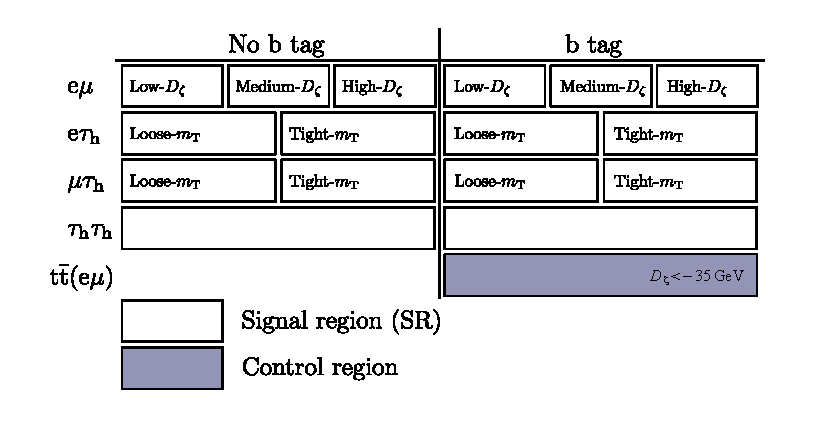
\includegraphics[width=0.85\textwidth]{Figures/high_mass_categories.pdf}
\caption[Diagram of the categories in the high-mass optimisation procedure.]{Overview of the categories used for the extraction of the signal in the high-mass optimisation procedure~\cite{CMS:2022rbd}.}
\label{fig:high_mass_categories}
\end{figure}

Once all category divisions have been applied, events are drawn in histograms based on a discriminating variable.
The discriminating variable used in this analysis is $m_{T}^{\text{tot}}$ and is defined below. \\
\begin{equation}
m_{T}^\text{tot} = \sqrt{m_{T}(\pTvec^{\hspace{2pt}\tau_1},\pTvec^{\hspace{2pt}\text{miss}})^2 +  m_{T}(\pTvec^{\hspace{2pt}\tau_2},\pTvec^{\hspace{2pt}\text{miss}})^2 + m_{T}(\pTvec^{\hspace{2pt}\tau_1},\pTvec^{\hspace{2pt}\tau_2})^2},
\label{eqn:mt_tot}
\end{equation} \\
where $\tau_1$ and $\tau_2$ refer to the visible products of the two $\tau$ lepton decays.
This variable provides excellent discriminating power between higher mass resonant signals compared to other non-peaking backgrounds, whilst still maintaining some separation between signal masses.
It is also excellent at separating the high-mass non-resonant di-$\tau$ signatures from backgrounds, where a di-$\tau$ mass does not represent the mass of a resonance.
This is due to the use of the transverse momenta and \ac{MET} in the variable definition.
For a t-channel signal where the mediator has high mass, no significant mass separation is expected in any variable. \\

\subsection{Low-mass optimisation}

The low-mass optimisation procedure, loosely follows the high-mass procedure with a few key differences.
Categories that are only sensitive to high-mass signals are dropped.
This includes the \texttt{Low-$D_\zeta$} and \texttt{Loose-$m_{T}$} categories.
Each no b tag subcategory is further divided into four bins of reconstructed di-$\tau$ visible $\pT$ with bin edges: 0, 50, 100, 200 and $\infty$.
This is not done in the b tag subcategories due to the lack of statistics in this region.
A schematic of the categories used in the low-mass optimisation procedure is shown in Figure~\ref{fig:low_mass_categories}.
The final difference with the high-mass optimisation procedure is the discriminator used.
In the low-mass optimisation procedure the reconstructed di-$\tau$ mass is used.
This helps to separate signal events from the Z boson peak in this region. \\

\subsection{Standard Model Higgs boson optimisation}

Finally, the \ac{SM} Higgs optimisation procedure is taken from the \ac{CMS} \ac{SM} $H \rightarrow \tau\tau$ analysis and is detailed in Reference~\cite{CMS:2022kdi}.
This was previously used for simplified template cross-section measurements.
This uses a \ac{NN}-based categorisation to obtain the most precise estimates from data of the \ac{SM} Higgs produced via gluon fusion, vector boson fusion or vector boson-associated production.
The \ac{NN} based analysis introduces 26 categories, 8 of which are optimised to pull out the Higgs boson signal.
Although the \ac{NN} is trained specifically to target events with an \ac{SM}-like Higgs boson, signal events with differing masses can also enter the \ac{NN} categories.

\begin{figure}[!hbtp]
\centering
    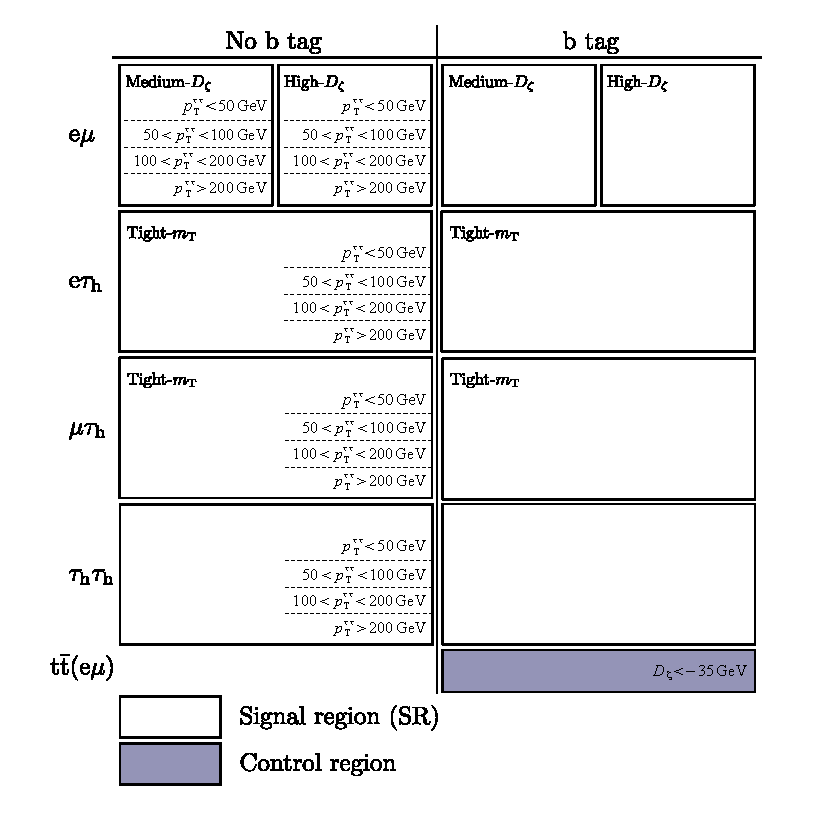
\includegraphics[width=0.85\textwidth]{Figures/low_mass_categories.pdf}
\caption[Diagram of the categories in the low-mass optimisation procedure.]{Overview of the categories used for the extraction of the signal in the low mass optimisation procedure~\cite{CMS:2022rbd}.}
\label{fig:low_mass_categories}
\end{figure}

\section{Background modelling overview}
\label{sec:background_modelling}

The relevant backgrounds for this analysis include $Z/\gamma^*$, $\ttbar$, W+jets, \ac{QCD}, di-boson, single-top, and electroweak W and Z bosons production.
These are split into five categories:
\begin{enumerate}[i)]
  \item Events containing only genuine $\tau$ leptons.
  \item Events with a jet misidentified as a $\tau_h$ (\jtth) in the $\etauh$, $\mutauh$ or $\tauhtauh$ channels.
  \item Events with jets misidentified as both light leptons ($\text{jet}\rightarrow \ell$) in the $\emu$ channel.
  \item Events from $\ttbar$ with a prompt light lepton ($e$ or $\mu$ not from a $\tau$ decay) and the other object (if there are not two prompt light lepton) is from a genuine $\tau$ lepton.
  \item Other events. This is a small contribution and so it is grouped.
  \begin{itemize}
    \item Non $\ttbar$ events satisfying (iv).
    \item Events with a light lepton misidentified as a $\tau_h$ and no \jtth candidate. 
    \item Events with a jet misidentified as a light lepton and the other object is from genuine $\tau$ leptons in the $\etauh$, $\mutauh$ or $\tauhtauh$ channels.
    \item Events with a muon misidentified as an electron in the $\emu$ channel.
    \item Events with one jet misidentified as a light lepton and the other object from a prompt light lepton in the $\emu$ channel.
   \end{itemize}
\end{enumerate}

Backgrounds from (i) consist of largely Z/$\gamma^* \rightarrow \tau\tau$ events but there are also smaller contributions from other processes. 
This background is modelled by a data-simulation hybrid method called the \say{embedding} method~\cite{CMS_embedding} and this is described in detail in Section~\ref{sec:embedding}.
Group (ii) is dominated by \ac{QCD}, W + jets and $\ttbar$ events with a \jtth misidentification.
This is modelled from data by the \say{fake factor} ($\FF$) method~\cite{Sirunyan:2018zut,CMS:2018lkr} and is explained in Section~\ref{sec:ff}.
Group (iii) is modelled from data to describe the \ac{QCD} multijet contribution to the background in the $\emu$ channel.
The method to obtain this background is described in Section~\ref{sec:qcd}.
The data-driven background estimations for (i), (ii) and (iii) contribute $\approx$98\% of all expected background events in the $\tauhtauh$ channel, $\approx$90\% in $\etauh$ and $\mutauh$ channels and $\approx$50\% in the $\emu$ channel.
The final groups, (iv) and (v), are modelled with \ac{MC} simulations.
The $\ttbar$ process from (iv) is separated because of its large contribution to the phase space where a b jet is required. \\

In 2016 (2017--2018), the W + jets and $Z\rightarrow \ell\ell$ processes are simulated using the \MGvATNLO 2.2.2 (2.4.2) event generator at \ac{LO}~\cite{Alwall:2011uj}. 
Supplementary samples are generated with up to four outgoing partons in the hard interaction to increase the number of simulated events in regions of high signal purity. 
For di-boson production, \MGvATNLO is used at \ac{NLO} precision~\cite{Alwall:2011uj}, and the FxFx~\cite{Frederix:2012ps} (MLM~\cite{Alwall:2007fs}) prescription is used to match the \ac{NLO} (\ac{LO}) matrix element calculation with the parton shower model. 
Samples for $\ttbar$~\cite{Alioli:2011as} and (t-channel) single top quark production~\cite{Frederix:2012dh} are generated at \ac{NLO} precision using \POWHEG 2.0~\cite{Nason:2004rx,Frixione:2007vw,Alioli:2010xd,Jezo:2015aia}, and for single top quark production in association with a W boson (tW channel)~\cite{Re:2010bp}, \POWHEG version 1.0 at \ac{NLO} precision is used. 
When compared with data, W + jets, $Z\rightarrow \ell\ell$, $\ttbar$, and single top quark events in the tW channel are normalised to their cross-sections at \ac{NNLO} precision\cite{Melnikov:2006kv,Czakon:2011xx,Kidonakis:2013zqa}, while single top quark and di-boson events are normalised to their cross-sections at \ac{NLO} precision or higher~\cite{Kidonakis:2013zqa,Campbell:2011bn,Gehrmann:2014fva}.

\section{QCD estimation in the $\emu$ channel}
\label{sec:qcd}

The \ac{QCD} model in the $\emu$ channel, which attempts to model events where two jets are misidentified as an electron-muon pair, is taken from data where the electron and muon have the same sign, with a transfer factor ($F_{T}$).
The transfer factor determines differences from the same sign to opposite sign region and is calculated from a sideband region with an anti-isolated muon ($0.2 < \Irel < 0.5$).
$F_{T}$ is initially parametrised by the $\Delta R$ between the electron and muon, and the number of jets in the event 
However, additional dependencies on the electron and muon $\pT$ enter via a correction. \\

Good agreement is observed in events with no b jets when applying $F_{T}$ onto same sign events compared to opposite sign events where both regions have an anti-isolated muon. 
However, in events with a b jet, an additional correction is needed.
This is determined to be $\approx$0.75 (differs very slightly between data-taking years).
As this correction is large, it is validated by switching the light lepton anti-isolation so that the election is required to have $0.15 < \Irel < 0.5$.
Also, events where both light leptons are anti-isolated are looked at.
The correction for b-tagged events is equivalent in all three regions, and a global average of the three is taken for the final correction. \\

To understand the physical reason for the large difference in no b tag and b tag events in same sign and opposite pairs, studies were performed on simulated samples.
It was observed that the electron-muon pair is usually produced from pairs of heavy quarks, $pp\rightarrow b\bar{b}$ ($c\bar{c}$).
If the two jets are initiated from the heavy quarks there is a large bias towards opposite sign jets due to the opposite signs of the quark-antiquark pair.
However, if one of the heavy quarks is tagged as a b jet, another object has to be the jet initiator (a radiated gluon for example) and there is therefore no charge preference in the pair.
As $F_{T}$ is originally fit inclusively in numbers of b jets and the 0 bin is dominant, the correction overpredicts the opposite sign to same sign ratio and so a large correction is needed as observed.

\section{Embedding method}
\label{sec:embedding}

The background for genuine di-$\tau$ lepton pairs is modelled via the embedding method~\cite{CMS_embedding}. 
This is a hybrid method that utilises both data and \ac{MC} techniques to produce high-statistic samples, where the bulk of the event comes from data.
This minimises both the chance of \ac{MC} fluctuations and the size of the uncertainties.
The genuine di-$\tau$ background is dominated by the $Z \rightarrow \tau \tau$ process, but there will be smaller contributions from $t\bar{t}$ and di-boson processes.  \\

The algorithm first selects $\mu\mu$ events from data.
The selection is chosen to naturally target the pure $Z \rightarrow \mu\mu$ region but still be loose enough to catch events from other processes, so as not to introduce a bias on the Z boson mass.
Events are required to pass the double-$\mu$ trigger with minimum requirements on the invariant mass of the two muons ($m_{\mu\mu}$) and the $\pT$ of the leading and trailing muons.
Also required at the trigger level is a loose association of the track to the \ac{PV} and a loose isolation in the tracker.
Offline objects matched to the trigger muons, are then required to have standard $d_z$ and $\eta$ selections and originate from a global muon track, as defined in Section~\ref{sec:object_reconstruction}.
The muon pair are required to have an opposite charge and have $m_{\mu\mu} > 20$ GeV.
The fraction of processes within this selection is tested with \ac{MC} background samples and a \ac{QCD} model from same sign muon pairs with an extrapolation factor.
Approximately 97\% of selected events are expected to come from $Z/\gamma^* \rightarrow \mu\mu$ events with smaller contributions from $Z/\gamma^* \rightarrow \tau\tau$ ($\tau\rightarrow\mu$), di-boson, $\ttbar$ and QCD.
The di-boson and $\ttbar$ relative contributions are greater at higher $m_{\mu\mu}$ and in events with tagged b jets, whilst the \ac{QCD} contribution is largest at lower $m_{\mu\mu}$.
The events selected are biased by detector acceptances. 
Therefore, corrections on the reconstruction and identification efficiencies are performed in muon $\eta$ and $\pT$ using the \say{tag-and-probe} method, as described in Reference~\cite{CMS:2010svw}. \\

Next, all energy deposits in the detector from the selected muons are removed.
This involves removing the hits on global muon tracks in the tracker, hits in the muon systems and clusters in the calorimeters that intercept the muon trajectory.
Once completed, the selected muons and their kinematic properties are replaced with simulated $\tau$ leptons.
To account for the difference in mass between the muon and $\tau$, the muons are boosted into the centre-of-mass frame of the di-muon system and then this four-vector is taken for the $\tau$ but boosted back into the laboratory frame.
The event simulation is performed from the \ac{PV}.
The $\tau$ lepton decay is then simulated with \PYTHIA~\cite{Sirunyan:2019dfx,Sjostrand:2014zea} and separate samples are produced for different $\tau\tau$ decay channels.
Only the decay of the $\tau$ leptons is then processed through the detector simulation and the remainder of the $\mu\mu$ event is added back.
A schematic of the process is shown in Figure~\ref{fig:embedding}. \\

\begin{figure}[!hbtp]
\centering
    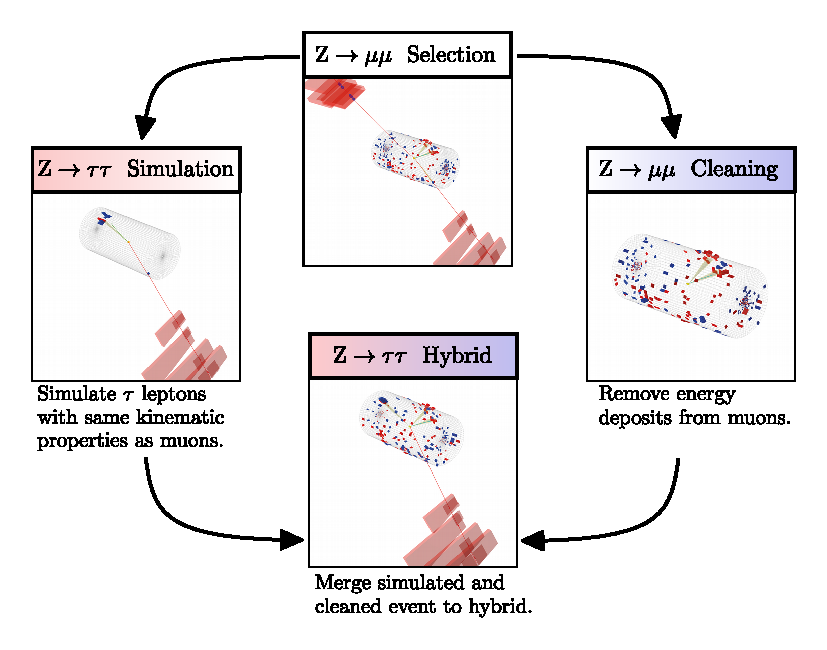
\includegraphics[width=0.9\textwidth]{Figures/Embedding_Diagram.pdf}
\caption[Diagram of the embedding method.]{Schematic of the embedding method to model genuine di-$\tau$ backgrounds from di-muon events in data~\cite{CMS_embedding}.}
\label{fig:embedding}
\end{figure}

The embedding method is validated on dedicated samples, where the muons from data are replaced by simulated muons instead of $\tau$ leptons.
A plot of the agreement from these dedicated samples with data is shown in Figure~\ref{fig:emb_validation}.

\begin{figure}[!hbtp]
\centering
    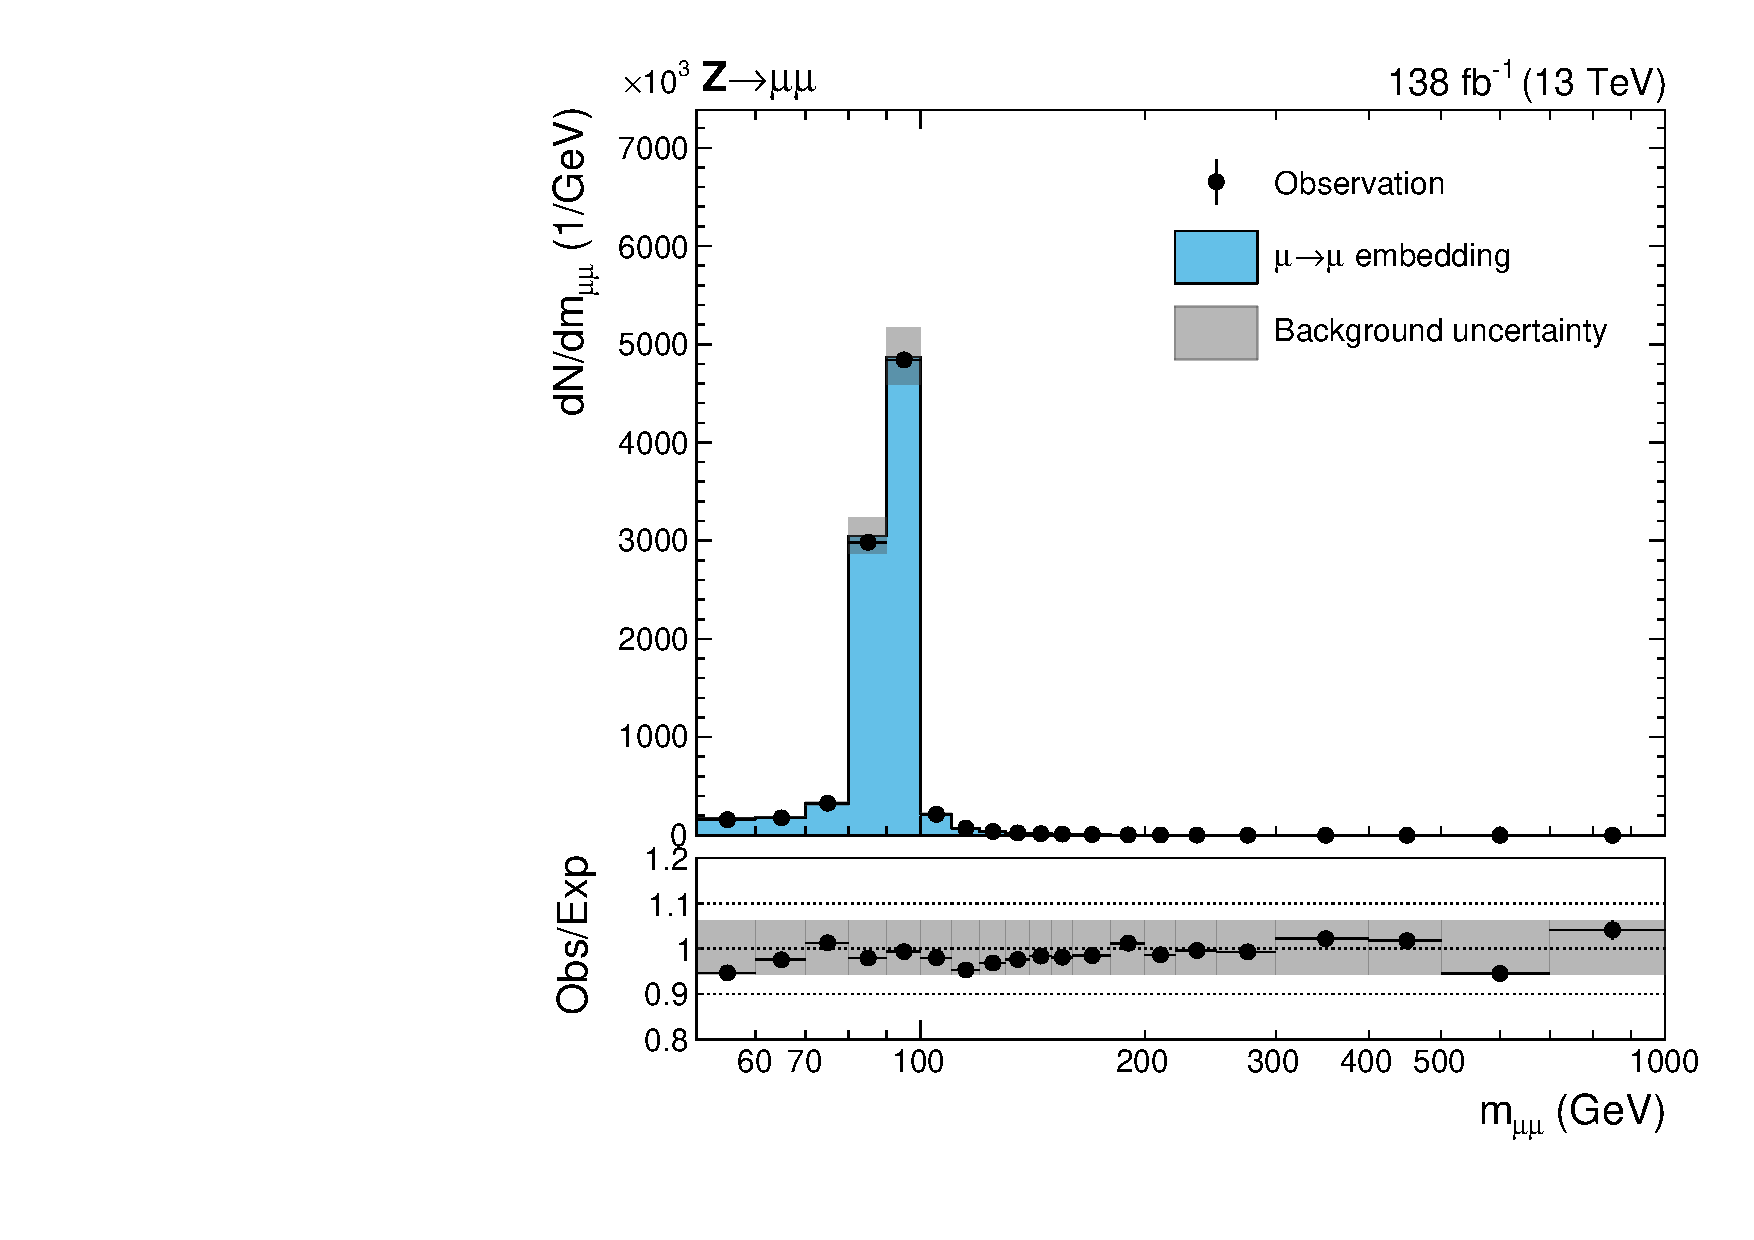
\includegraphics[width=0.7\textwidth]{Figures/embedding_validation.pdf}
\caption[Plot of the validation of the embedding method.]{Closure plot showing the di-muon mass on the dedicated embedding validation samples.}
\label{fig:emb_validation}
\end{figure}

\section{Fake factor method}
\label{sec:ff}

Backgrounds in which a jet is misidentified as a $\tauh$ can be difficult to model using \ac{MC} due to the poor description of the \jtth fake rate in simulation. 
In addition, the small probability of a jet being misidentified as a $\tauh$ necessitates the production of high statistics \ac{MC} samples at a significant computational expense.
These shortcomings motivate the use of data-driven estimations for these processes. 
One such procedure is the $\FF$ method~\cite{Sirunyan:2018zut,CMS:2018lkr}. \\

The $\FF$ method utilises regions in the data to model the \jtth background. 
Firstly, the determination regions are defined, which are \jtth enriched regions orthogonal to the signal region. 
They are then purified by subtracting off any non \jtth events with \ac{MC}.
It is used to calculate a $\FF$ by taking the ratio of the number of \jtth events that pass the nominal $\tau_h$ identification requirement ($N(\texttt{Nominal})$), to the number of \jtth events that fail the nominal $\tau_h$ identification but pass a looser alternative $\tau_h$ identification requirement ($N(\texttt{Alternative}\text{ and not }\texttt{Nominal})$), as shown in Equation~\ref{eqn:ff}.

\begin{equation}
\FF = \frac{N(\texttt{Nominal})}{N(\texttt{Alternative}\text{ and not }\texttt{Nominal})}.
\label{eqn:ff}
\end{equation}

In the remaining text, this numerator and denominator are referred to as the pass and fail regions.
The derivation of this ratio is done differentially with respect to key parameters that differ in the two regions.
Once $\FF$ have been derived it is common to calculate corrections in other sideband regions and combine $\FF$ measured from different processes.
Finally, the $\FF$ are applied to the application region. 
This is defined as the signal region but with the criteria that the \jtth events fail the nominal $\tau_h$ identification but pass the looser alternative $\tau_h$ identification requirement.
This now models the background from \jtth events in the signal region. \\

The following Sections~\ref{sec:ff_dr}--\ref{sec:ff_applying} detail the complexities of how this method is applied to this analysis.
For these searches, the nominal $\tau_h$ identification used is the \texttt{Medium} $D_{\text{jet}}^{\text{WP}}$ and the alternative $\tau_h$ identification used is the \texttt{VVVLoose} $D_{\text{jet}}^{\text{WP}}$.

\subsection{Determination regions}
\label{sec:ff_dr}

The $\FF$ are measured separately in each year of data taking period (2016, 2017, 2018), in each channel containing a $\tau_h$ ($\etauh$, $\mutauh$, $\tauhtauh$) and in enriched regions of dominant processes that contribute \jtth events.
In the $\etauh$ and $\mutauh$ channels $\FF$ are measured for three processes: \ac{QCD}, W + jets and $\ttbar$.
In the $\tauhtauh$ channel $\FF$ are measured only for the dominant \ac{QCD} process.
The \ac{QCD} process is assumed to produce two jets misidentified as $\tauh$ candidates, and so the $\FF$ is chosen to be calculated from leading $\pT$ $\tau_h$ candidate only.
Section~\ref{sec:ff_applying} discusses how a single \jtth events in the $\tauhtauh$ channel are modelled. \\

Each separate measurement region is split into three sideband regions based on two cuts that surround the signal region.
These regions are named the \texttt{Determination Region} (A), \texttt{Alternative Determination Region} (B) and \texttt{Correction Region} (D) and are schematically shown in Figure~\ref{fig:ff_schematic}. \\

\begin{figure}[!hbtp]
\centering
    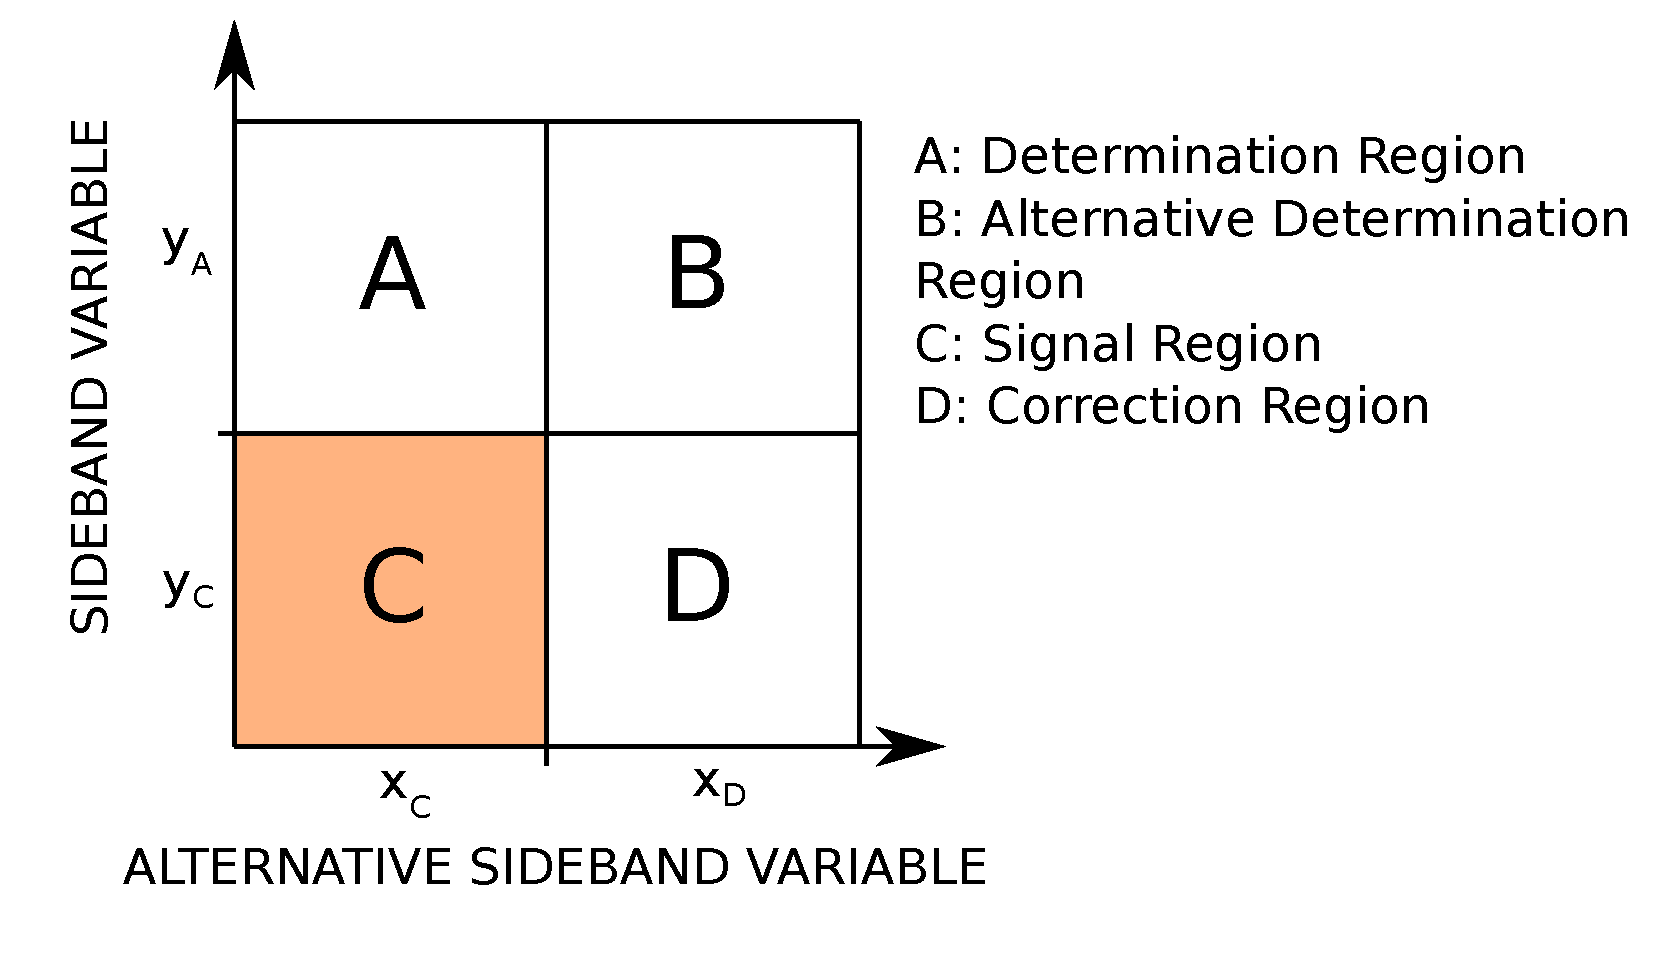
\includegraphics[width=0.8\textwidth]{Figures/ff_diagram_v2.pdf}
\caption[Diagram of the regions used for fake factor derivation.]{Schematic of the regions used for fake factor derivation.}
\label{fig:ff_schematic}
\end{figure}

Region A is used to measure and fit the $\FF$.
Region B is an alternative region used to measure and fit the $\FF$ to account for the difference between A and C.
These alternative $\FF$ are applied to the fail $\tauh$ identification region in D and corrections are calculated by comparing it to the pass region in D.
The total $\FF$ per measurement region is calculated as the product of the $\FF$ derived in region A and the correction calculated from region B to D. \\

The selection for $x_C$, $x_D$, $y_C$ and $y_A$, as defined in Figure~\ref{fig:ff_schematic}, in each separate measurement region are shown below.
These are chosen to balance the number of events and the purity of each background in the region.

\begin{enumerate}[i)]
   \item $\tauhtauh$ \ac{QCD} \\
     \indent $y_C$: The $\tauh$ candidates are required to have the opposite sign. \\
     \indent $y_A$: The $\tauh$ candidates are required to have the same sign. \\
     \indent $x_C$: The subleading $\tau_h$ passes the \texttt{Medium} $D_{\text{jet}}^{\text{WP}}$. \\
     \indent $x_D$: The subleading $\tau_h$ fails the \texttt{VVLoose} $D_{\text{jet}}^{\text{WP}}$ but passes the \texttt{VVVLoose} $D_{\text{jet}}^{\text{WP}}$.
  \item $\etauh$ and $\mutauh$ \ac{QCD} \\
    \indent $y_C$: The $e$/$\mu$ and $\tauh$ candidates are required to have the opposite sign. \\
    \indent $y_A$: The $e$/$\mu$ and $\tauh$ candidates are required to have the same sign and the $e$/$\mu$ to have $\Irel>0.05$. \\
    \indent $x_C$: The $e$/$\mu$ candidate is required to have $\Irel<0.15$. \\
    \indent $x_D$: The $e$/$\mu$ candidate is required to have $0.25<\Irel<0.5$.
  \item $\etauh$ and $\mutauh$ W + Jets \\
    \indent $y_C$: The $\mT$ between the $e$/$\mu$ and the \ac{MET} $< 70$ GeV. \\
    \indent $y_A$: The $\mT$ between the $e$/$\mu$ and the \ac{MET} $> 70$ GeV and no b jets in the event. \\
    \indent $x_C$: Data. \\
    \indent $x_D$: W + Jets \ac{MC}.
  \item $\etauh$ and $\mutauh$ $\ttbar$ \\
    \indent $y_C$: Data. \\
    \indent $y_A$: \ac{MC} ($\ttbar$ in B and W + Jets D). \\
    \indent $x_C$: $\mT < 70$ GeV. \\
    \indent $x_D$: $\mT > 70$ GeV and no b jets. \\
\end{enumerate}


In the $\mu\tauh$ and $e\tauh$ channels, W + jets \jtth events are in general the most significant and \ac{QCD} contributes a smaller fraction. 
$\ttbar$ inclusively is small but becomes more significant when searching for events with a b jet. 
The additional $\Irel>0.05$ requirement in these channels for \ac{QCD} is to reduce processes producing genuine leptons and the $N_{\text{b jets}}=0$ requirement for W + Jets is to reduce $\ttbar$ contamination.
It is not possible to define a \texttt{Determination Region} that is sufficiently pure in $\ttbar$ events to make a reasonable measurement of $\FF$ from data.
Therefore, $\ttbar$ $\FF$ are derived from \ac{MC}. 
A comparison of the W + jets $\FF$ measured in data and \ac{MC} shows only $\sim$ 10--20\% differences in the fake rates in data and \ac{MC}.  
This observation coupled with the fact that the $\ttbar$ contribution is small compared to the other processes means that any bias introduced by using $\FF$ measured in \ac{MC} is small compared to the uncertainties on the $\FF$, discussed in Section~\ref{sec:uncerts}. 
In many cases, selections on the regions B and D are applied which are tighter than required, to purify the regions as much as possible, while maintaining enough statistics to perform the fit.\\


\subsection{Parametrisation}
\label{sec:ff_params}

The raw $\FF$ take into account dependencies on $N_{\text{jets}}$ via an analysis-category tailed variable $N_{\text{pre b jets}}$, the $\pT$ of the $\tauh$ candidate ($\pT^{\tauh}$) and the $\pT$ of the jet that seeds the \ac{HPS} algorithm ($\pT^{\text{jet}}$).
$N_{\text{pre b jets}}$ is the number of jets in the event with $|\eta|<2.4$ and $\pT>20$ GeV, which is the $\eta$ and $\pT$ selection for a b-tagged jet. 
It is defined to map the dependence of $\FF$ on the number of jets and describe the categorising variable $N_{\text{b jets}}$ well.
Although not local to the $\tauh$, it helps control other dependencies on the constituents of the event.
It is the number of jets in the event with $|\eta|<2.4$ and $\pT>20$ GeV. 
These are the same $\eta$ and $\pT$ thresholds required for a b jet.
The data is split into two bins of $N_{\text{pre b jets}}$, equal to 0 and greater than 0.
It is then further split by the ratio of $\pT^{\text{jet}}$ to $\pT^{\tauh}$.
An example of the dependence of these two transverse momentums on the fake factor is shown in Figure~\ref{fig:ff_colz}. \\

\begin{figure}[!hbtp]
\centering
    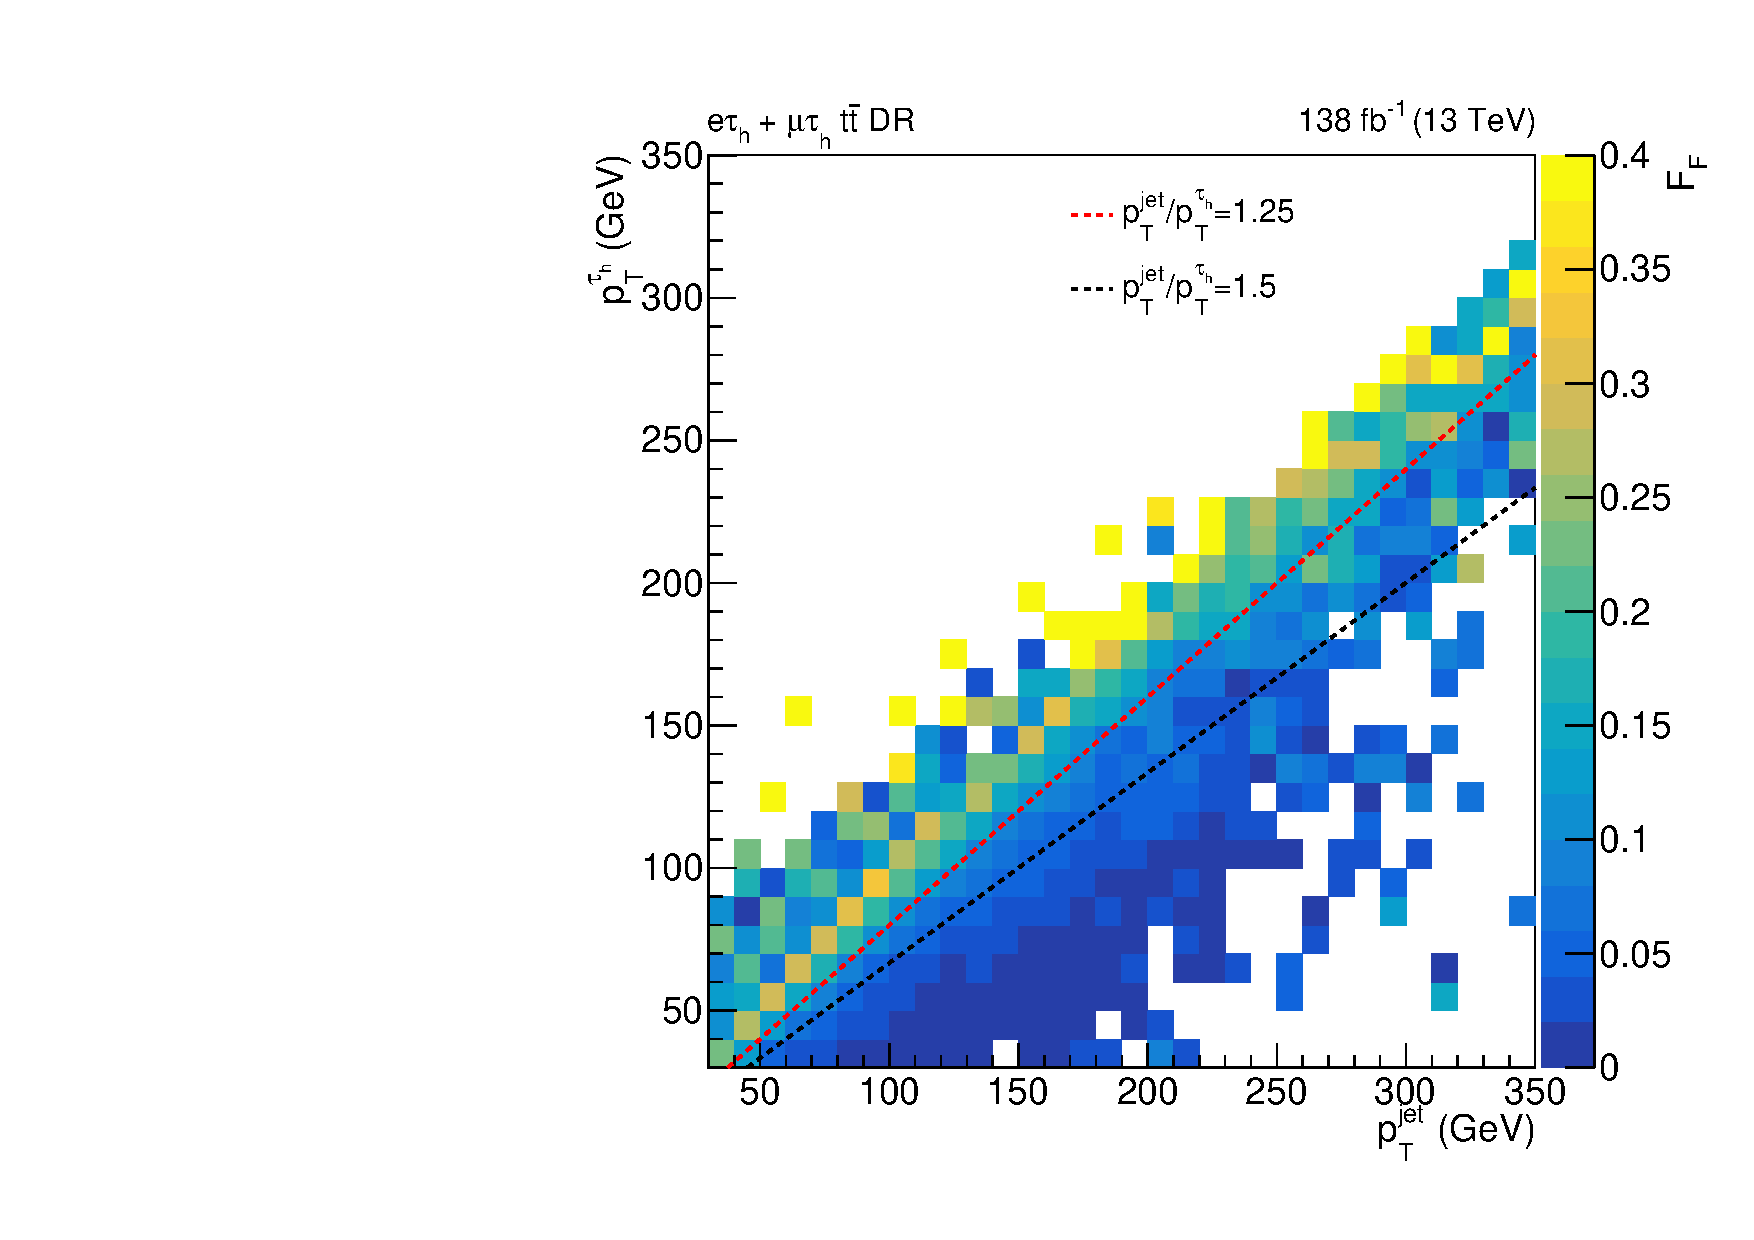
\includegraphics[width=0.6\textwidth]{Figures/ff_colz_ttbar_lt_v2.pdf}
\caption[Plot of the reliance of the fake factors on the ratio of the $\tauh$ and jet $\pT$.]{A 2D heat map of the $\FF$ determined from $t\bar{t}$ MC for the full Run 2 dataset in the combined $e\tauh$ and $\mu\tauh$ channels. This is shown with respect to the $\tau_h$ $\pT$ and the $\pT$ of the HPS seeded jet for the $\tauh$. The ratio of jet to $\tau_h$ $\pT$ categorisation used is shown split by the dashed lines.}
\label{fig:ff_colz}
\end{figure}

It is motivated by the observation that the $\FF$ are largest when the $\pT^{\text{jet}}$ and $\pT^{\tauh}$ are closest.
The physical motivation for this is when they are close, the $\tauh$ candidate is likely to be isolated from any other hadronic activity and so more likely to be identified as a $\tau$.
However, when $\pT^{\text{jet}}$ is larger than $\pT^{\tauh}$, the candidate is likely surrounded by other hadronic activity and so more likely to be a jet fake.
When $\pT^{\text{jet}}$ is less than $\pT^{\tauh}$, charged pions are likely not close enough to the \ac{PV} to be clustered into the jet and so the event is less likely to be classified as a $\tauh$. 
This leads to the $\FF$ dependence as seen in Figure~\ref{fig:ff_colz}.\\

For all divisions of the phase space, dependence on the $\pT^{\tauh}$ is fit using the superposition of a Landau function and a constant in the low-$\pT$ region.
The $\FF$ are seen to rise sharply at high $\pT$.
This increase happens in either the bin 140 $<$ $\pT^{\tauh}$ $<$ 200 GeV or $\pT^{\tauh}$ $>$ 200 GeV.
To map this effect, binned values are taken based on the algorithm shown in Figure~\ref{fig:ff_binning} and the fit is used below the minimum bin.

\begin{figure}[!hbtp]
  \centering
  \begin{tikzpicture}[node distance = 8cm, auto]
    % nodes
    \node [block] (start) {Fractional Error in $\pT$ (GeV) Bin, $\frac{\Delta N}{N}$.};
    \node [decision, aspect=2, node distance=5cm, right of = start] (d1) {[140,200)};
    \node [decision, aspect=2, node distance=3cm, above of = d1] (d2) {[200,$\infty$)};
    \node [decision, aspect=2, node distance=3cm, below of = d1] (d3) {[200,$\infty$)};
    \node [block3, aspect=2, node distance=3cm, above of = d2] (n1) {Use bin values in [140,200,$\infty$)};
    \node [block3, aspect=2, node distance=3cm, below of = d3] (n2) {Use bin values in [200,$\infty$)};
    \node [block3, aspect=2, node distance=5cm, right of = d2] (n3) {Use bin values in [140,$\infty$)};
    \node [block3, aspect=2, node distance=5cm, right of = d3] (n4) {Use no bins};
    % edges
    \draw [arrow] (start) -- (d1);
    \draw [arrow] (d1) -- node[anchor=east] {$>0.5$} (d2);
    \draw [arrow] (d1) -- node[anchor=east] {$<0.5$} (d3);
    \draw [arrow] (d2) -- node[anchor=east] {$>0.5$} (n1);
    \draw [arrow] (d2) -- node[anchor=south] {$<0.5$} (n3);
    \draw [arrow] (d3) -- node[anchor=east] {$>0.5$} (n2);
    \draw [arrow] (d3) -- node[anchor=south] {$<0.5$} (n4);
  \end{tikzpicture}
  \vspace{1cm}
  \caption[Diagram of the algorithm used to choose the binned values taken at high $\pT$ during the fake factor fitting.]{Flow chart of the algorithm used to determine where binned values are taken instead of the fit. The blue box represents the input, the green diamonds represent the decisions and the red boxes represent the outputs.}
  \label{fig:ff_binning}
\end{figure}

The fits are flattened at $\pT^{\tau_h}$ values where there is no significant downward shift or at the final bin to avoid extrapolating past the fitted range. 
$\FF$ fits with respect to $\pT^{\tau_h}$ are shown in Figures~\ref{fig:tt_ff_fit}-\ref{fig:mt_ff_fit}. 
The $\FF$ are highest in the lowest $\pT^{\text{jet}}/\pT^{\tau_h}$ bin and lowest in the highest $\pT^{\text{jet}}/\pT^{\tau_h}$ bin, as expected. 
Otherwise, the $\FF$ fall with $\pT$ in each category until the thresholds used for the high $\pT$ binning algorithm.

\begin{figure}[!hbtp]
\centering
    \subfloat[]{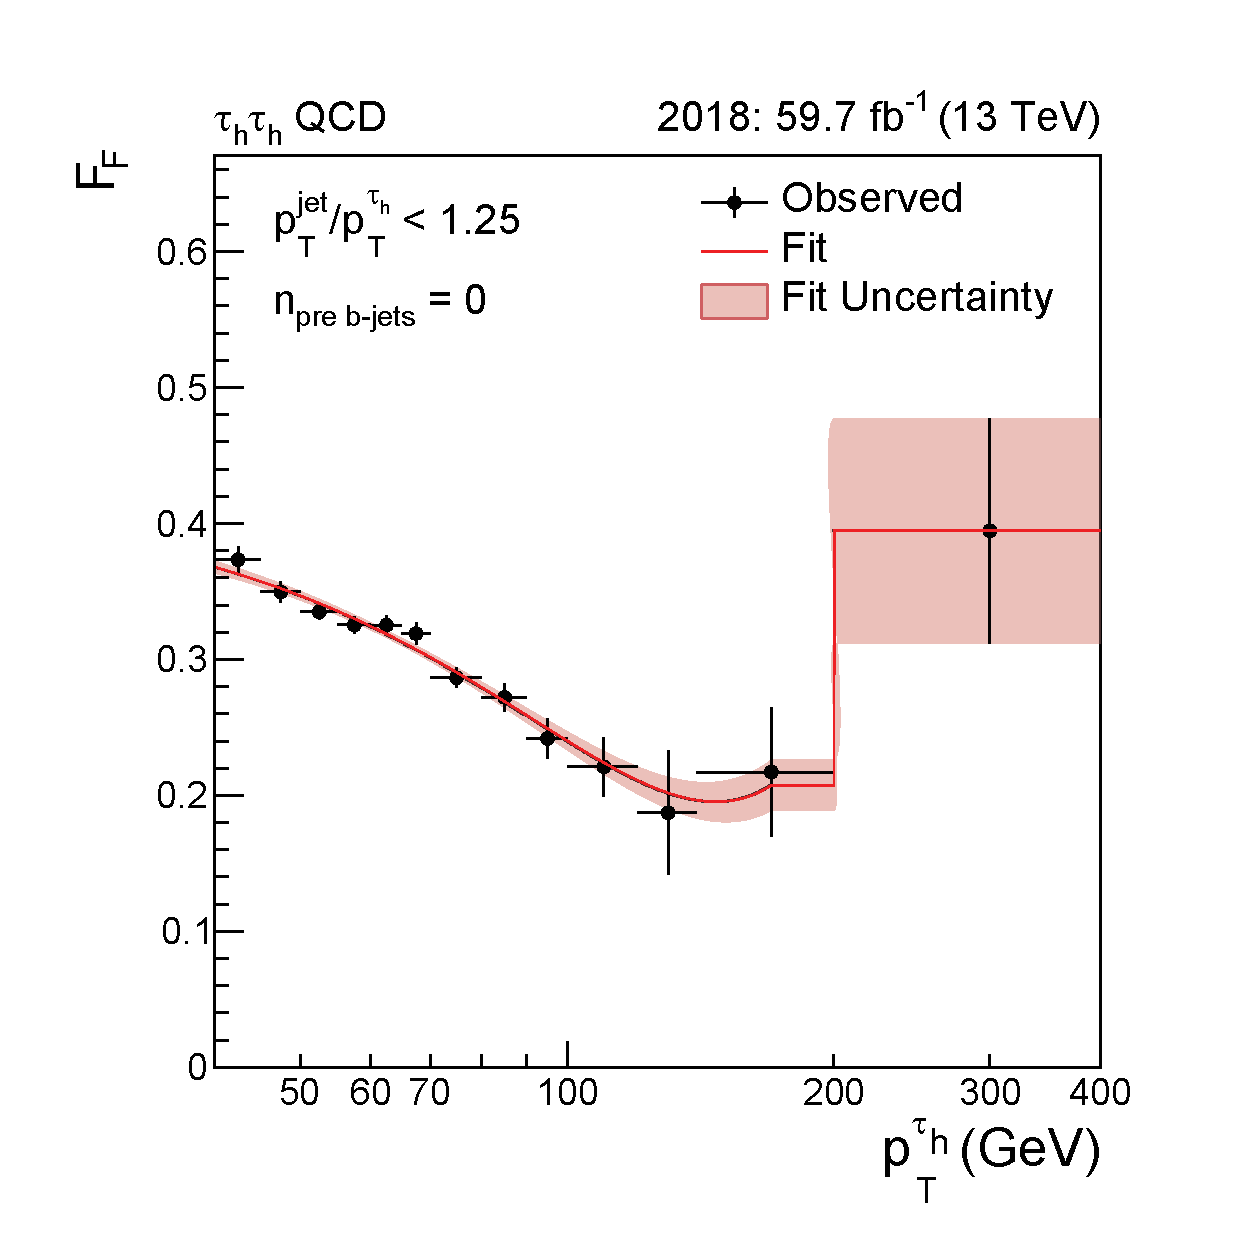
\includegraphics[width=0.33\textwidth]{Figures/ff_fit_jet_pt_low_0jet_pt_1_ff_qcd_tt_2018-EK.pdf}}
    \subfloat[]{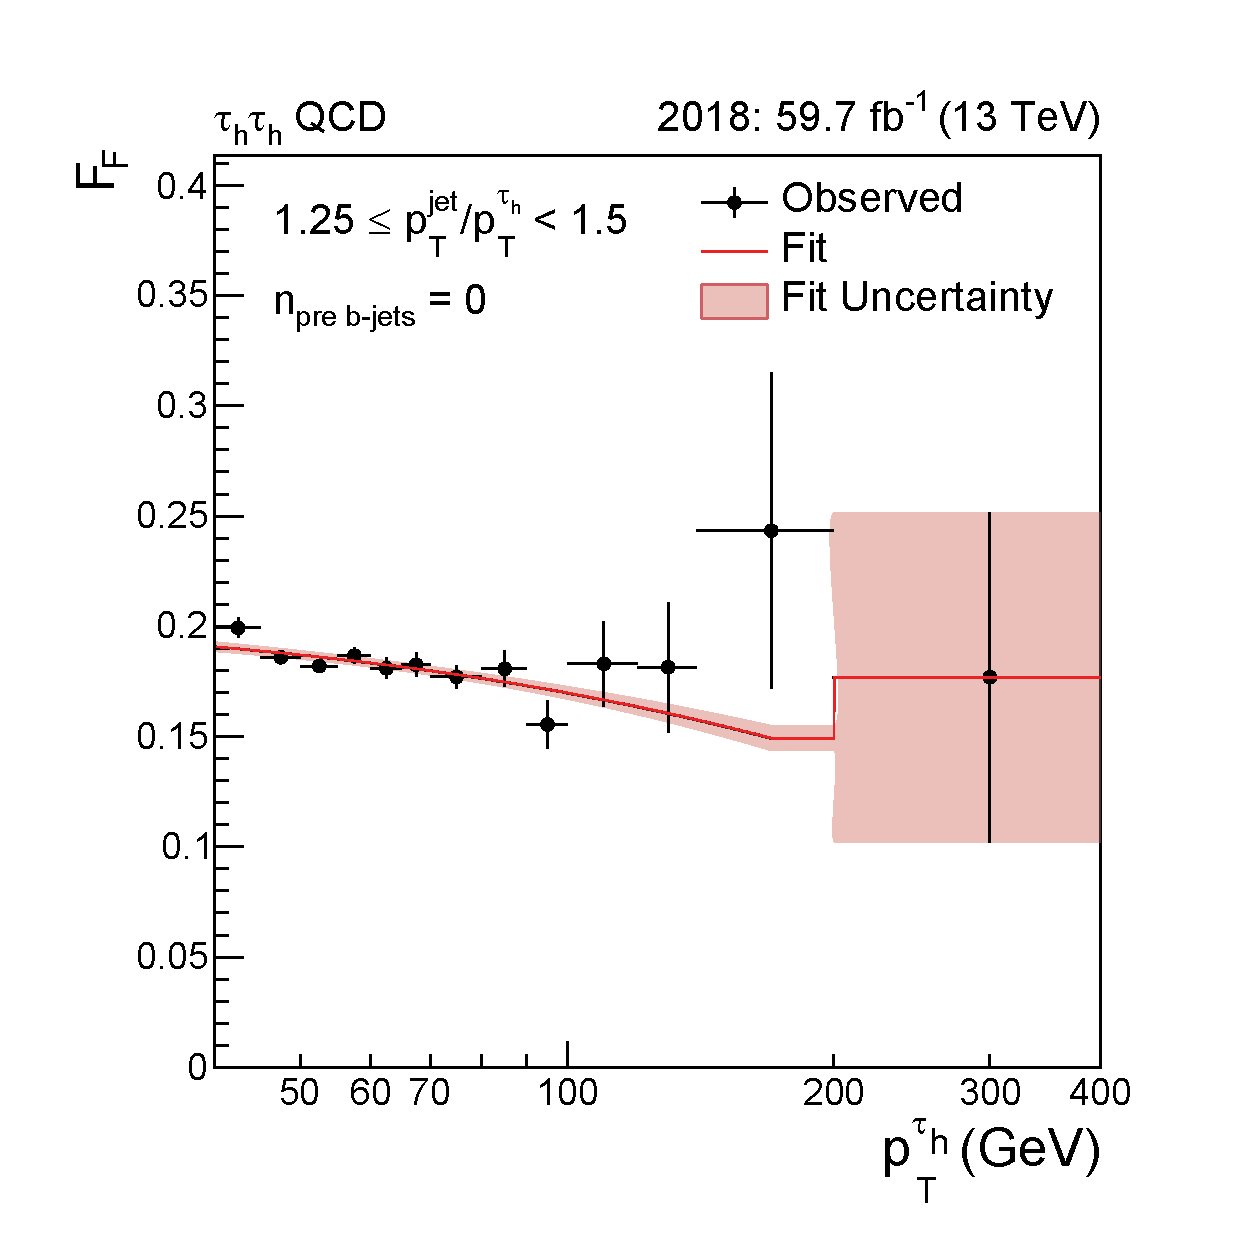
\includegraphics[width=0.33\textwidth]{Figures/ff_fit_jet_pt_med_0jet_pt_1_ff_qcd_tt_2018-EK.pdf}} 
    \subfloat[]{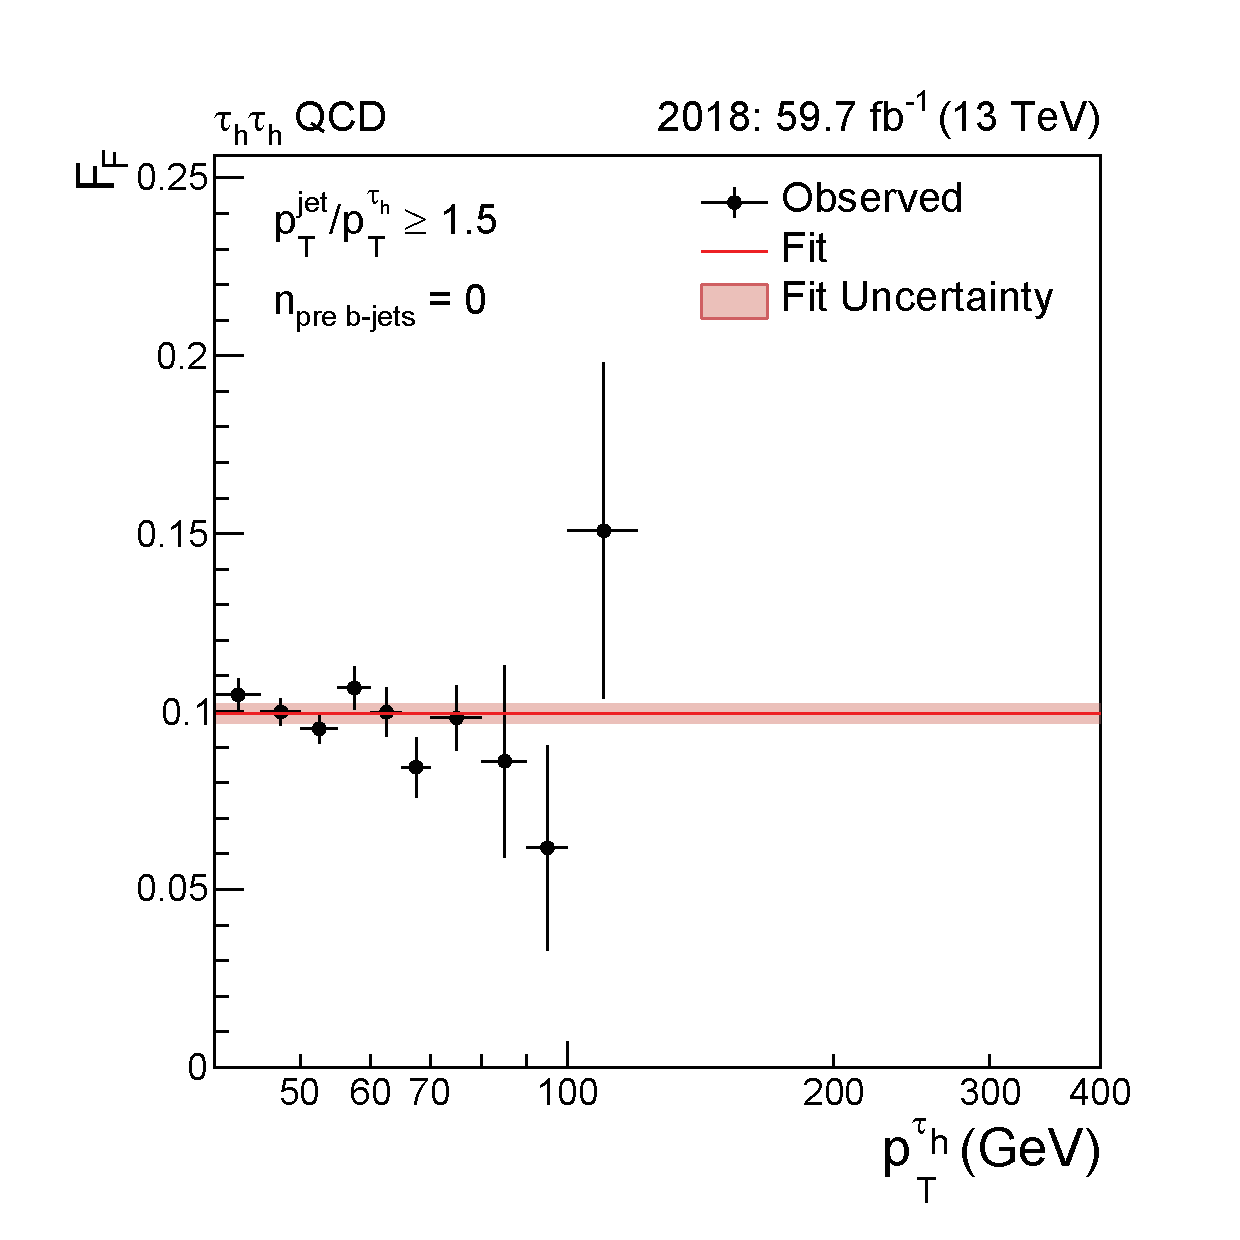
\includegraphics[width=0.33\textwidth]{Figures/ff_fit_jet_pt_high_0jet_pt_1_ff_qcd_tt_2018-EK.pdf}} \\
\caption[Plots of the fake factor fits in the $\tauh\tauh$ channel.]{$\FF$ fits in $\tauh\tauh$ channel for the QCD $N_{\text{pre b jets}}=0$ category with 2018 data. The three jet $\pT$ to $\tau_h$ $\pT$ categories are shown.}
\label{fig:tt_ff_fit}
\end{figure}

\begin{figure}[!hbtp]
\centering
    \subfloat[]{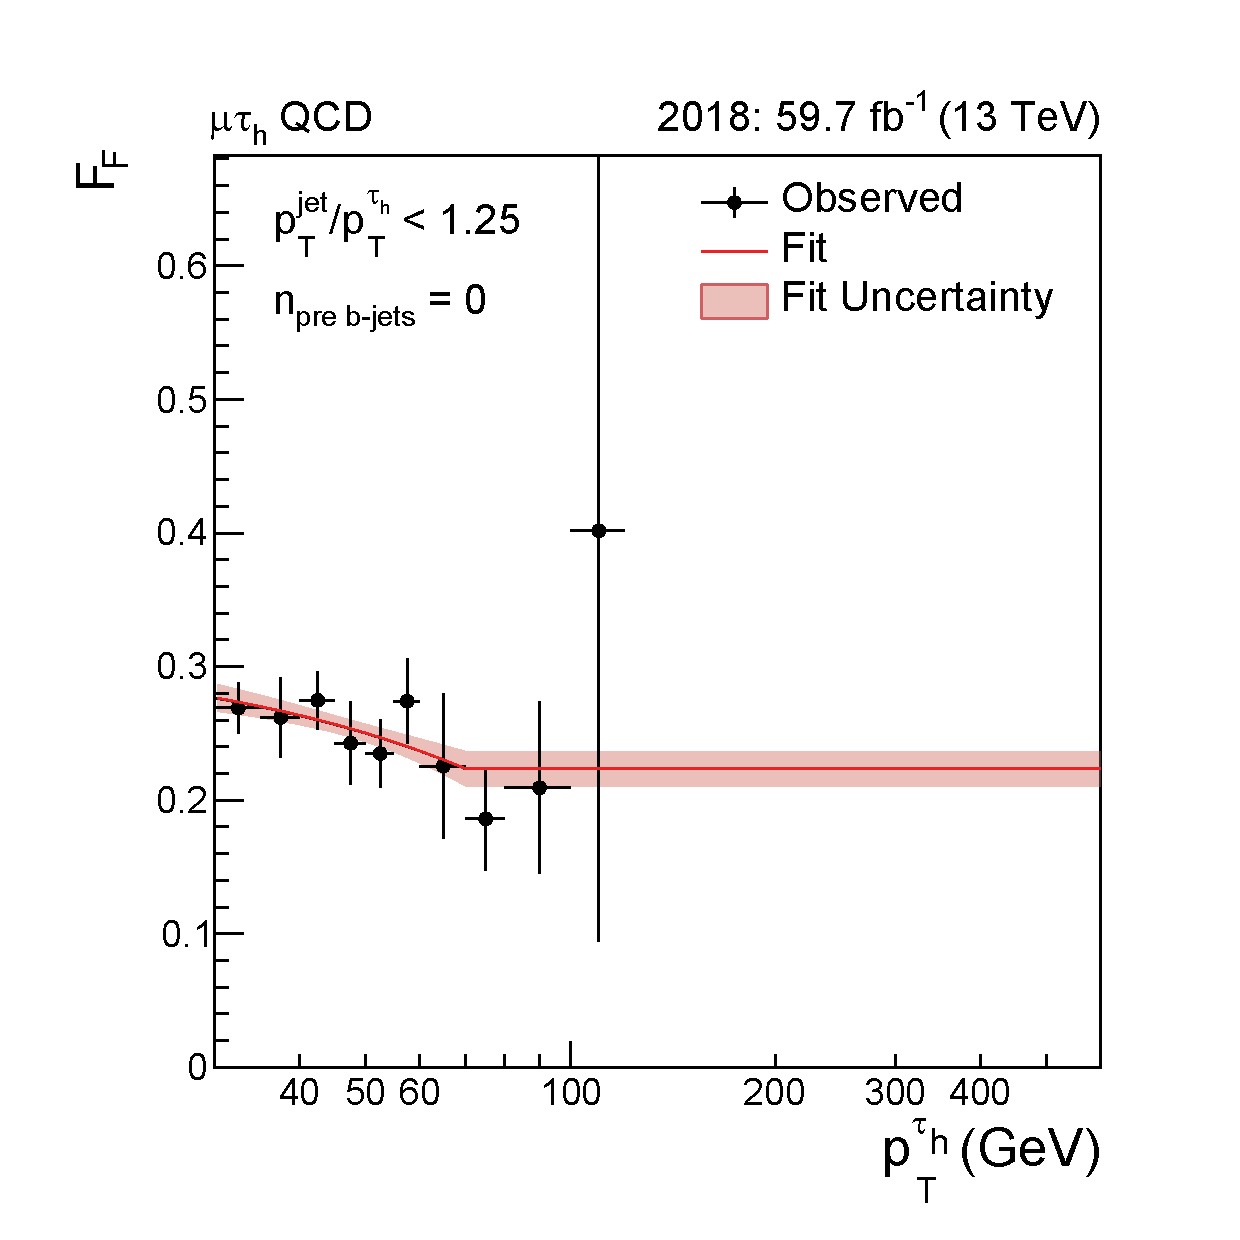
\includegraphics[width=0.33\textwidth]{Figures/ff_fit_jet_pt_low_0jet_pt_2_ff_qcd_mt_2018-EK.pdf}}
    \subfloat[]{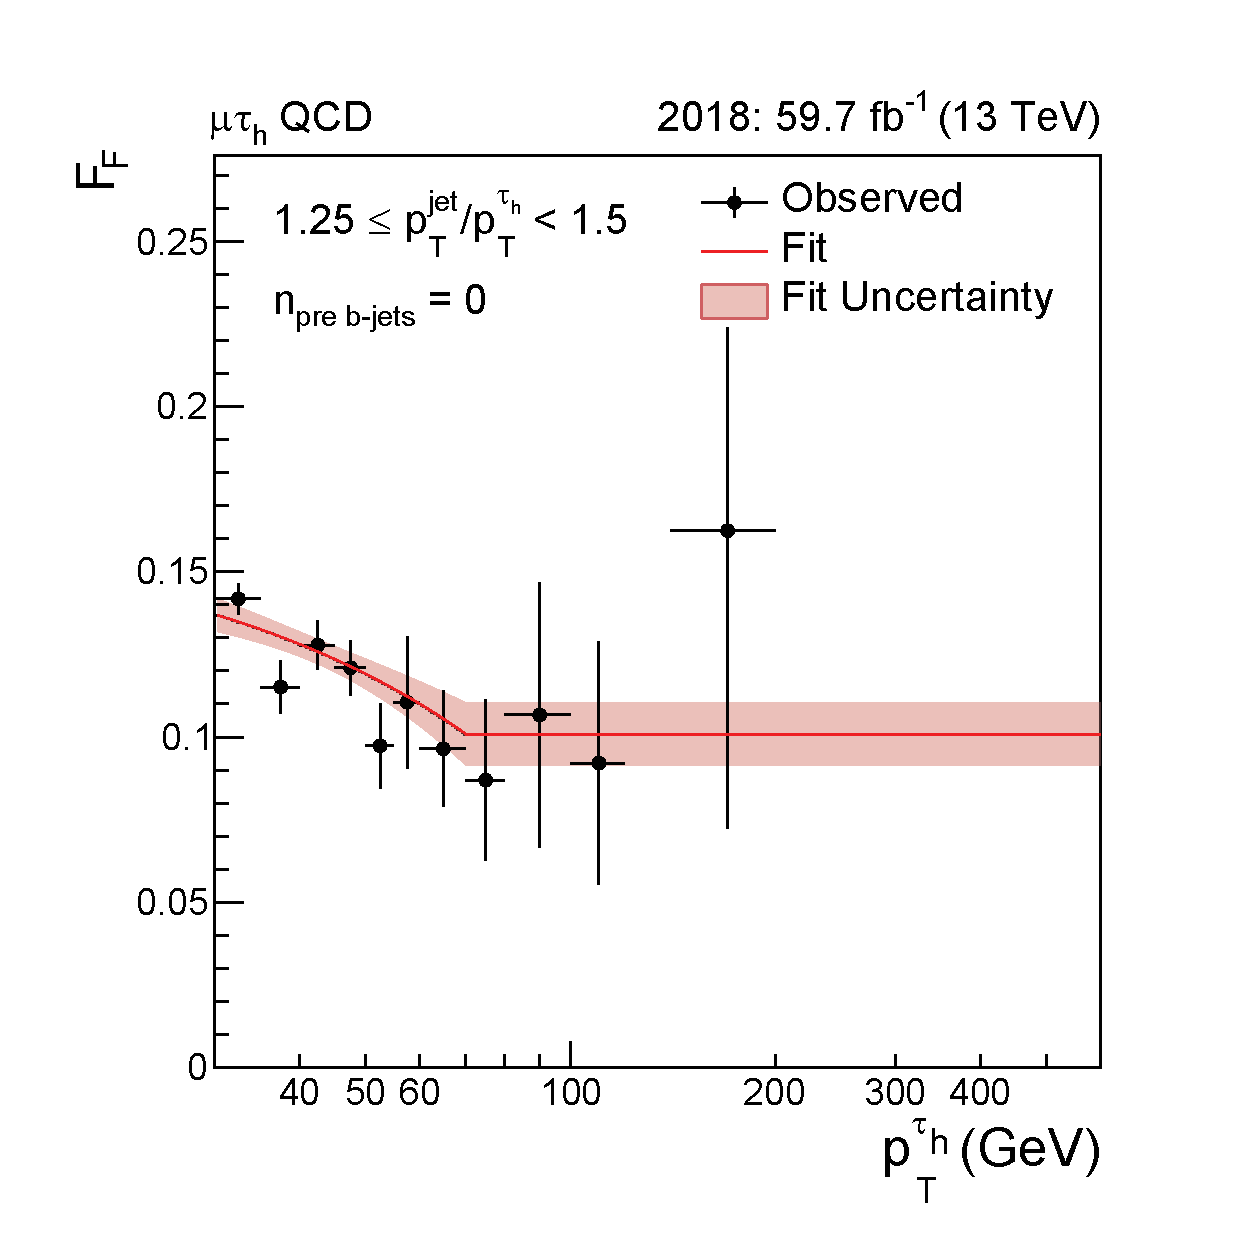
\includegraphics[width=0.33\textwidth]{Figures/ff_fit_jet_pt_med_0jet_pt_2_ff_qcd_mt_2018-EK.pdf}} 
    \subfloat[]{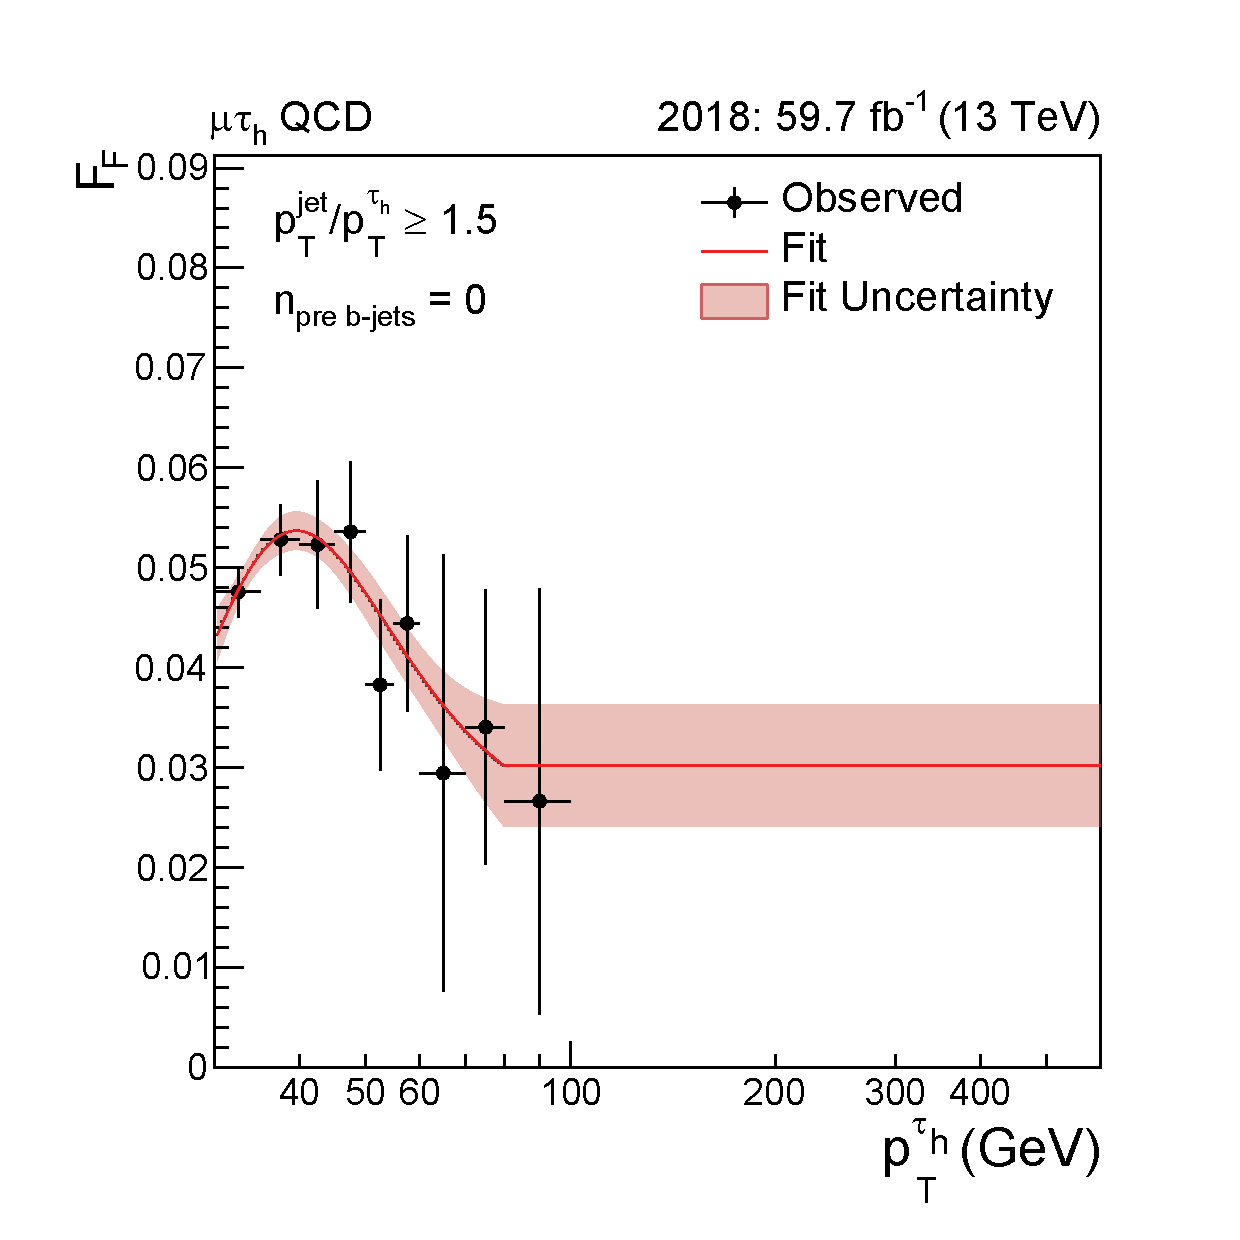
\includegraphics[width=0.33\textwidth]{Figures/ff_fit_jet_pt_high_0jet_pt_2_ff_qcd_mt_2018-EK.pdf}} \\
    \subfloat[]{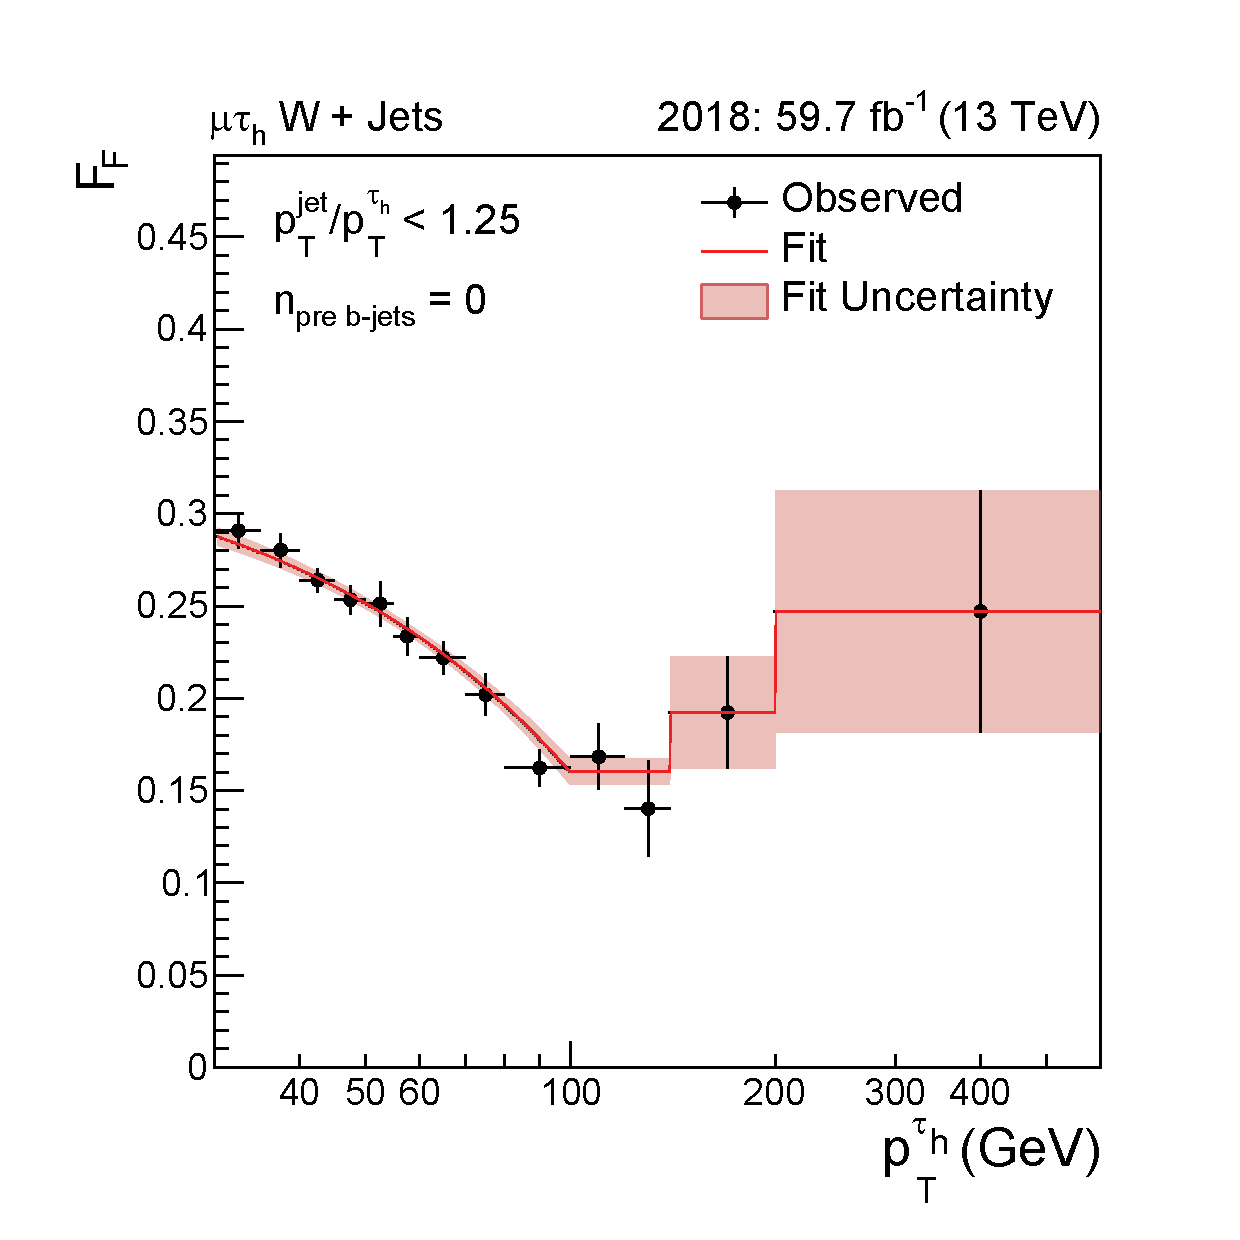
\includegraphics[width=0.33\textwidth]{Figures/ff_fit_jet_pt_low_0jet_pt_2_ff_wjets_mt_2018-EK.pdf}}
    \subfloat[]{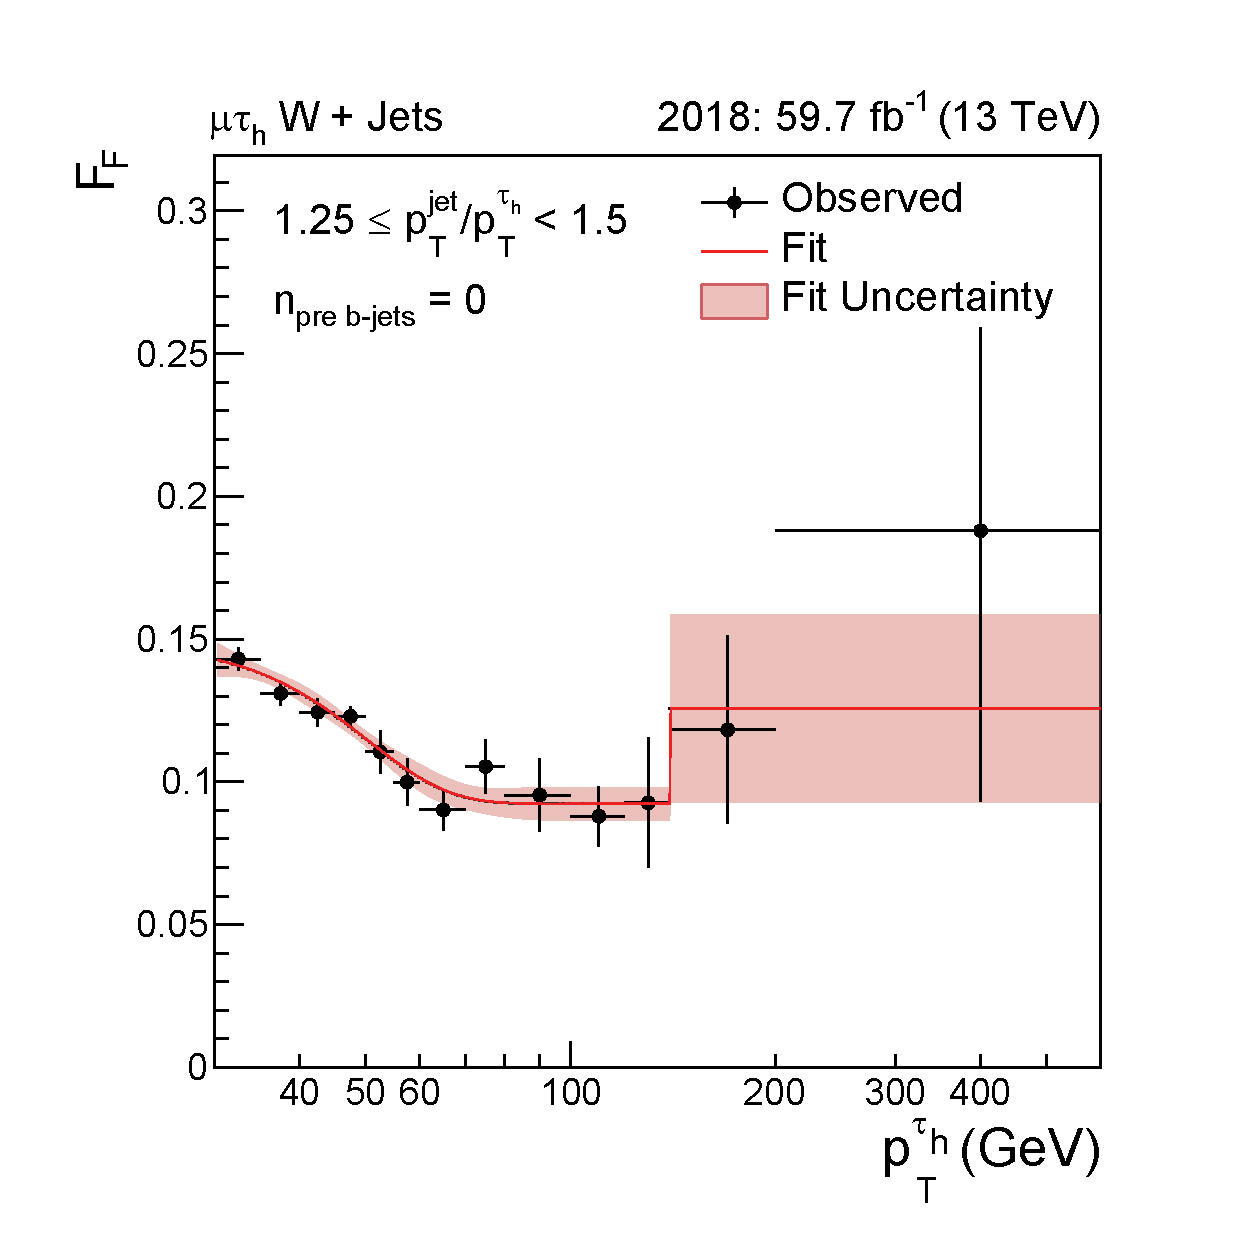
\includegraphics[width=0.33\textwidth]{Figures/ff_fit_jet_pt_med_0jet_pt_2_ff_wjets_mt_2018-EK.pdf}} 
    \subfloat[]{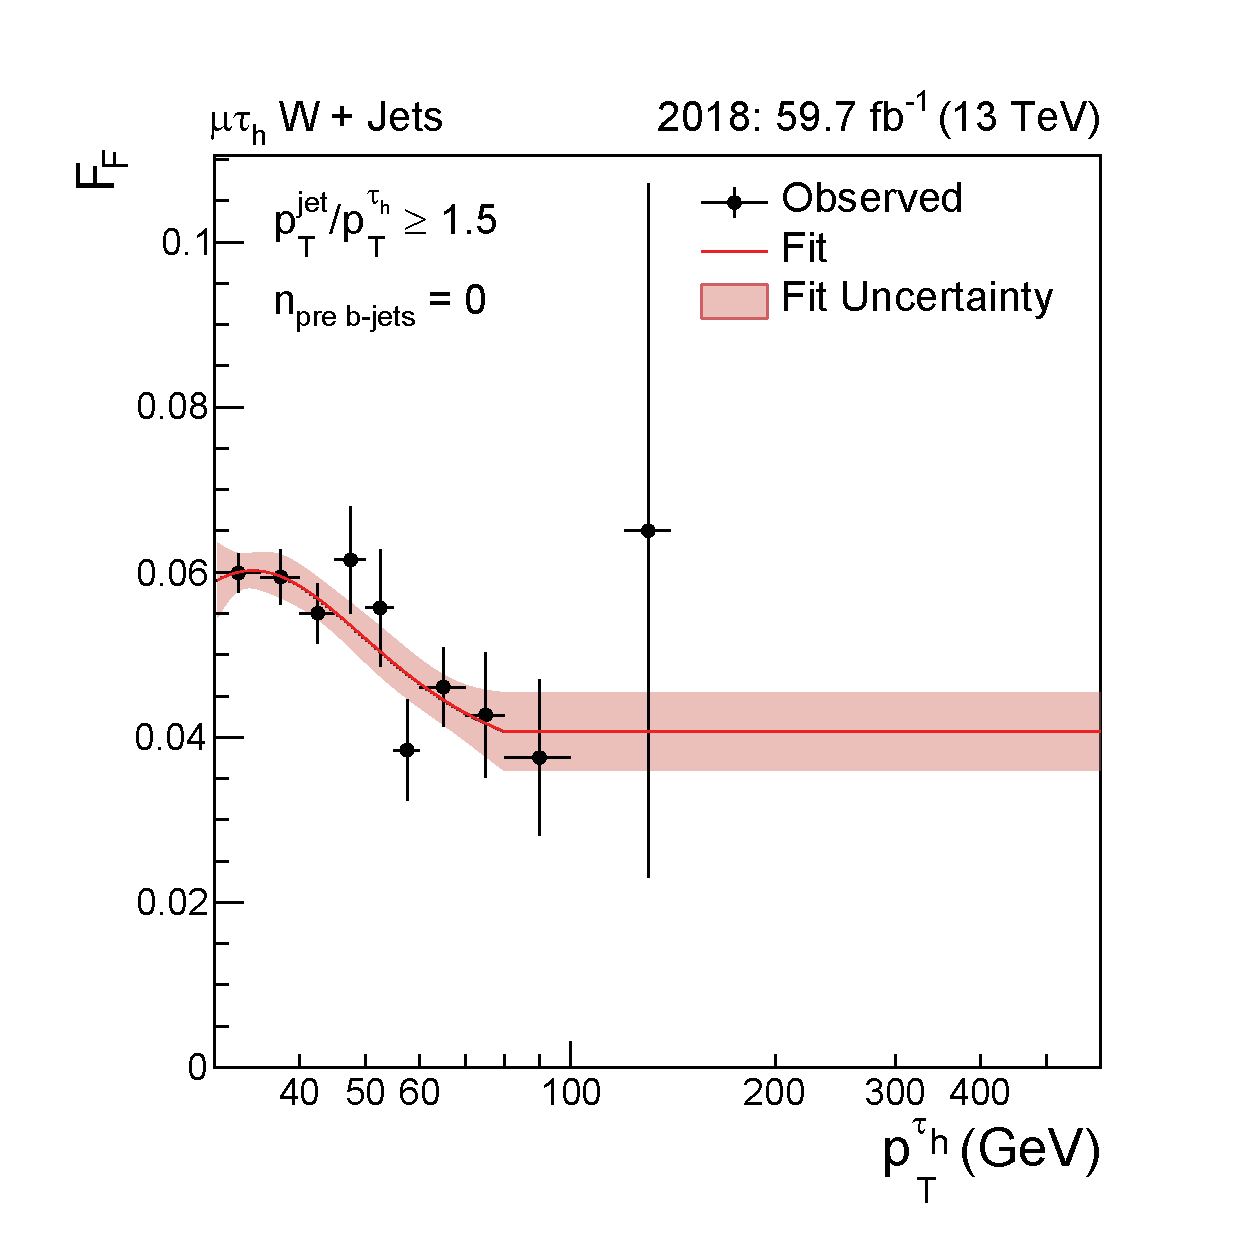
\includegraphics[width=0.33\textwidth]{Figures/ff_fit_jet_pt_high_0jet_pt_2_ff_wjets_mt_2018-EK.pdf}} \\
\caption[Plots of the fake factor fits in the $\mu\tauh$ channel.]{$\FF$ fits in $\mu\tauh$ channel for the QCD and W + Jets $N_{\text{pre b jets}}=0$ category with 2018 data. The three jet $\pT$ to $\tau_h$ $\pT$ categories are shown for each process.}
\label{fig:mt_ff_fit}
\end{figure}

\subsection{Corrections}

In the $\tauhtauh$ channel, the measured $\FF$ are then corrected to account for non-closures in other variables in the \texttt{Determination Region}. 
The only significant non-closures are observed for $\MET$ related variables and are largest for events with $N_{\text{pre b jets}}=0$. 
Closure corrections are performed for the variable $\Delta R$ between the $\tauh$ candidates in bins of $N_{\text{b jets}}$.
In the $\mutauh$ and $\etauh$ channels, the measured QCD and W + jets $\FF$ are corrected for non-closures observed in the $\MET$ variables and $\pT^{e/\mu}$ distributions.
A study was performed to determine the nature of these non-closures and it was found that the cause was due to fake \ac{MET} arising from mismeasurement of the energies of particles in a jet. 
If a jet's energy is mismeasured, this is also propagated to the reconstruction of the \ac{MET} and the $\tauh$ candidate and there will be a specific alignment between these objects if no neutrinos are present in the event.
A mismeasurement of the jet energy can alter the $\tauh$ isolation and so it can also affect the identification scores, and this shift can be accounted for with some measure of the fake \ac{MET}.
A diagram of this effect is shown in Figure~\ref{fig:fakemet}. \\

\begin{figure}[!hbtp]
\centering
   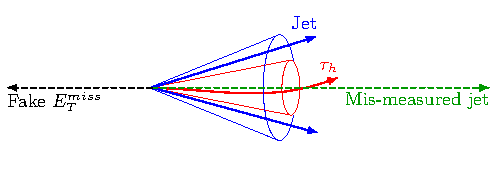
\includegraphics[width=\textwidth]{Figures/fakemet_plot.pdf}
\caption[Diagram of the fake MET alignment with the $\tauh$ candidate.]{Diagram showing how fake MET arises from mis-modelling jet energies and how it can align with the $\tauh$ candidate identified.}
\label{fig:fakemet}
\end{figure}

To correct for this effect, the QCD $\FF$ are corrected as a function of $C_{\text{QCD}}$, where $C_{\text{QCD}}$ is defined as,
\begin{equation}
C_{\text{QCD}} = \frac{\MET \cos\Delta\phi(\pTvec^{\text{\hspace{2pt}miss}},\pTvec^{\hspace{2pt}\tauh})}{\pT^{\tauh}}.
\label{eqn:c_qcd}
\end{equation}
where $\Delta\phi(\pTvec^{\hspace{2pt}\text{miss}},\pTvec^{\hspace{2pt}\tauh})$ is the separation in the azimuthal angle between the missing transverse momentum vector $\pTvec^{\hspace{2pt}\text{miss}}$ and $\pTvec^{\hspace{2pt}\tauh}$.
The numerator quantifies the missing transverse momentum in the direction of the $\tau_h$ candidate. 
Once divided by the $\tauh$ $\pT$, $C_{\text{QCD}}$ is a measure of the fraction of missing to visible $\tau_h$ transverse momentum aligned with the $\tau_h$.
For W + jets and $\ttbar$ the situation is slightly different due to the presence of genuine missing energy from neutrinos.
In this case, the correction variable is modified to approximately subtract the genuine \ac{MET} from the total.
This approximation assumes the neutrino is back-to-back and balanced with the light lepton (which is exactly true for W bosons produced at rest in the transverse direction). 
The equation then becomes,
\begin{equation}
C_{\text{W}} = \frac{(\MET+\pT^{e/\mu}) \cos\Delta\phi(\pTvec^{\text{\hspace{2pt}miss}}+\pTvec^{\hspace{2pt}e/\mu},\pTvec^{\hspace{2pt}\tauh})}{\pT^{\tauh}}.
\label{eqn:c_w}
\end{equation}
When either correction variable is non-zero, a larger quantity of fake \ac{MET} is expected in the event. 
In these regions, a large correction is needed due to the mismeasured jet energy spectrum shifting the $\tau_h$ candidate isolation and so shifting the $\tau$ identification scores. 
Examples of these closure corrections are shown in Figure~\ref{fig:ff_dr}\\

After the \texttt{Determination Region} is modelled well for all variables of interest, extrapolation corrections from the $\FF$ derived in B applied to region D are calculated.
In the $\tauhtauh$ the correction is parametrised by the $p_{T}$ of the leading $\tau_h$ candidate, in the $\etauh$ and $\mutauh$ channels it is parametrised by the $\pT$ of the light lepton.
Where statistics allow, these corrections are calculated in the high-mass optimisation procedure categories.
Examples of the extrapolation corrections are shown in Figure~\ref{fig:ff_dr_to_ar}.

\begin{figure}[!hbtp]
\centering
    \subfloat[]{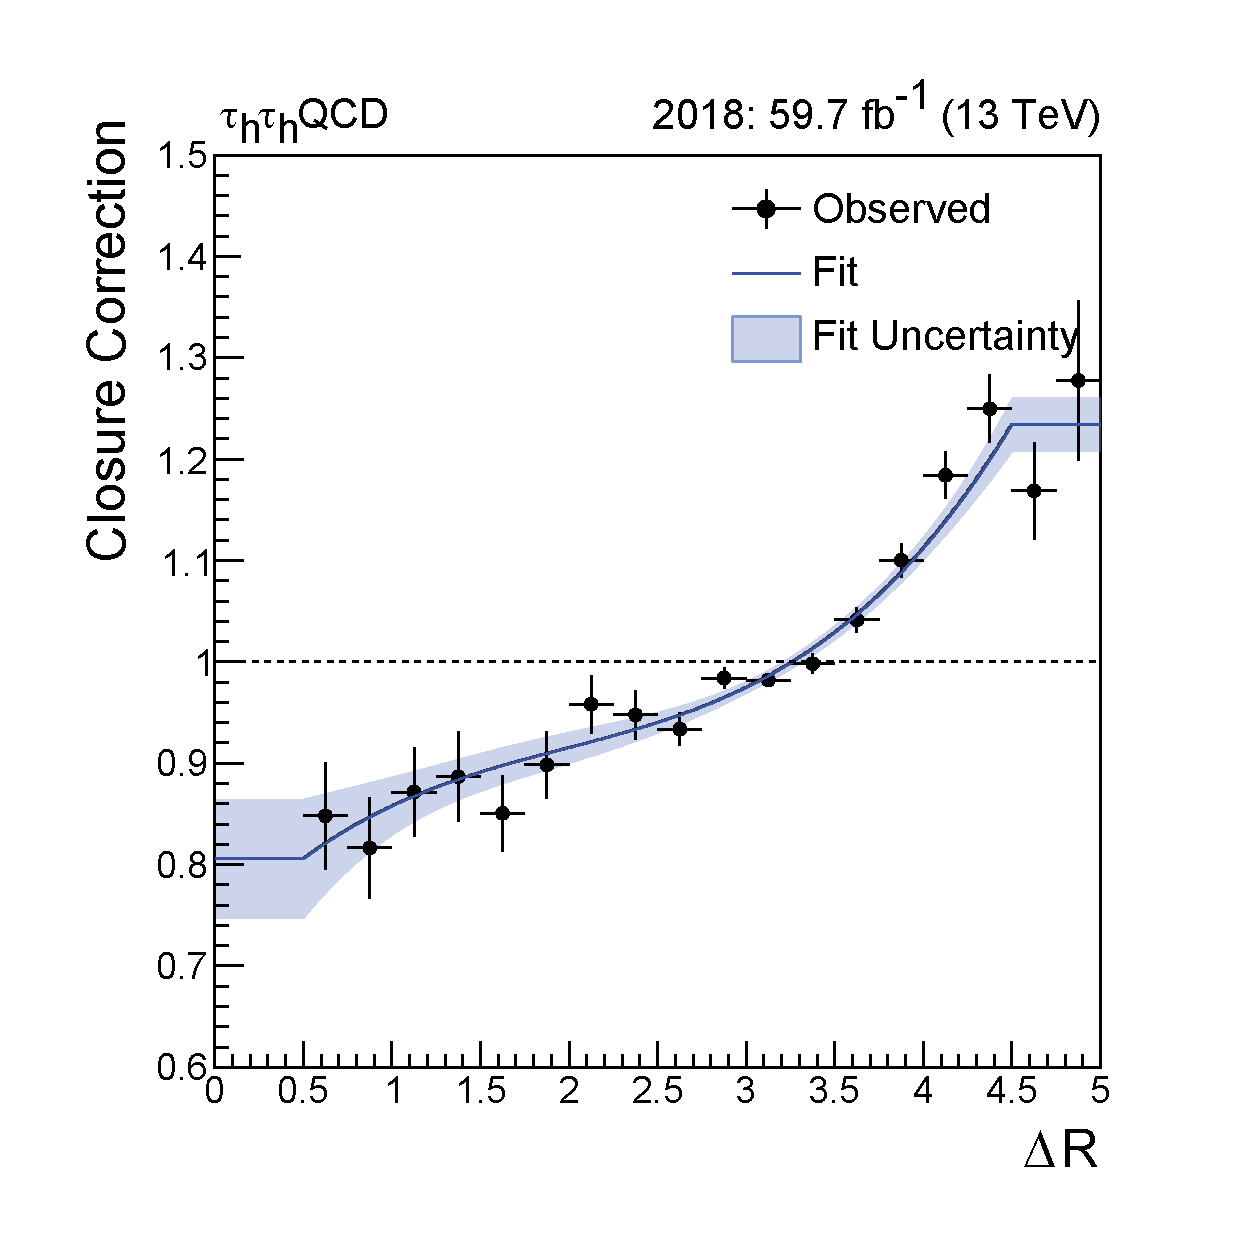
\includegraphics[width=0.33\textwidth]{Figures/ff_closure_ss_closure_nbjet0_qcd_tt_2018_v2-EK.pdf}} 
    \subfloat[]{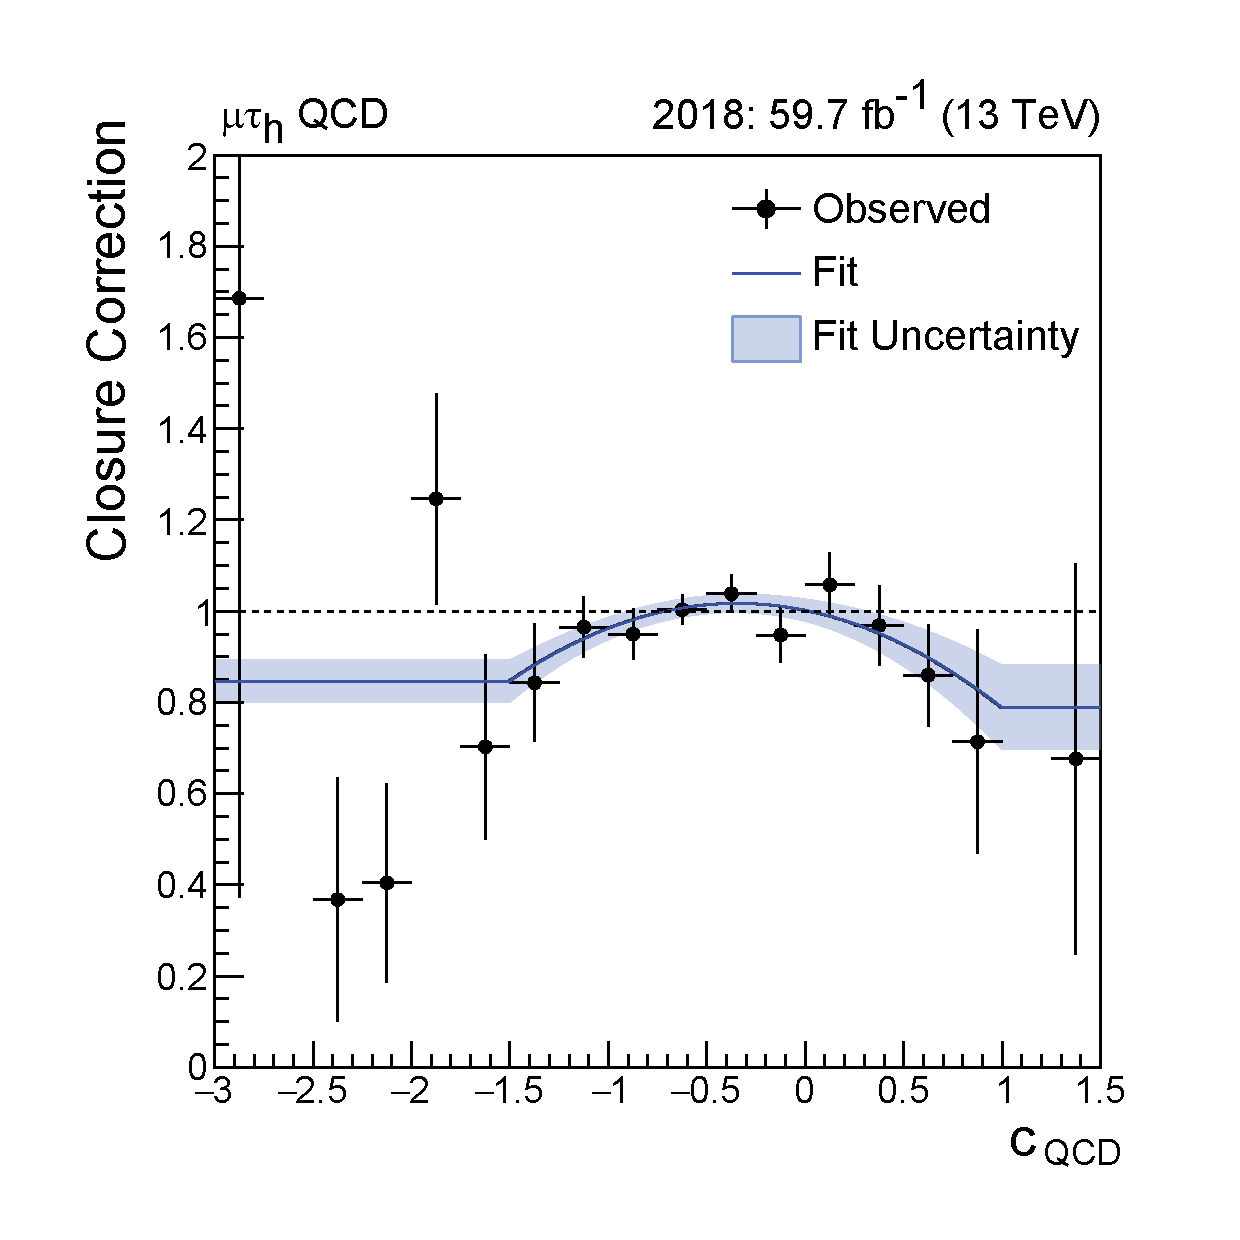
\includegraphics[width=0.33\textwidth]{Figures/ff_closure_met_0jet_closure_qcd_mt_2018-EK.pdf}}
    \subfloat[]{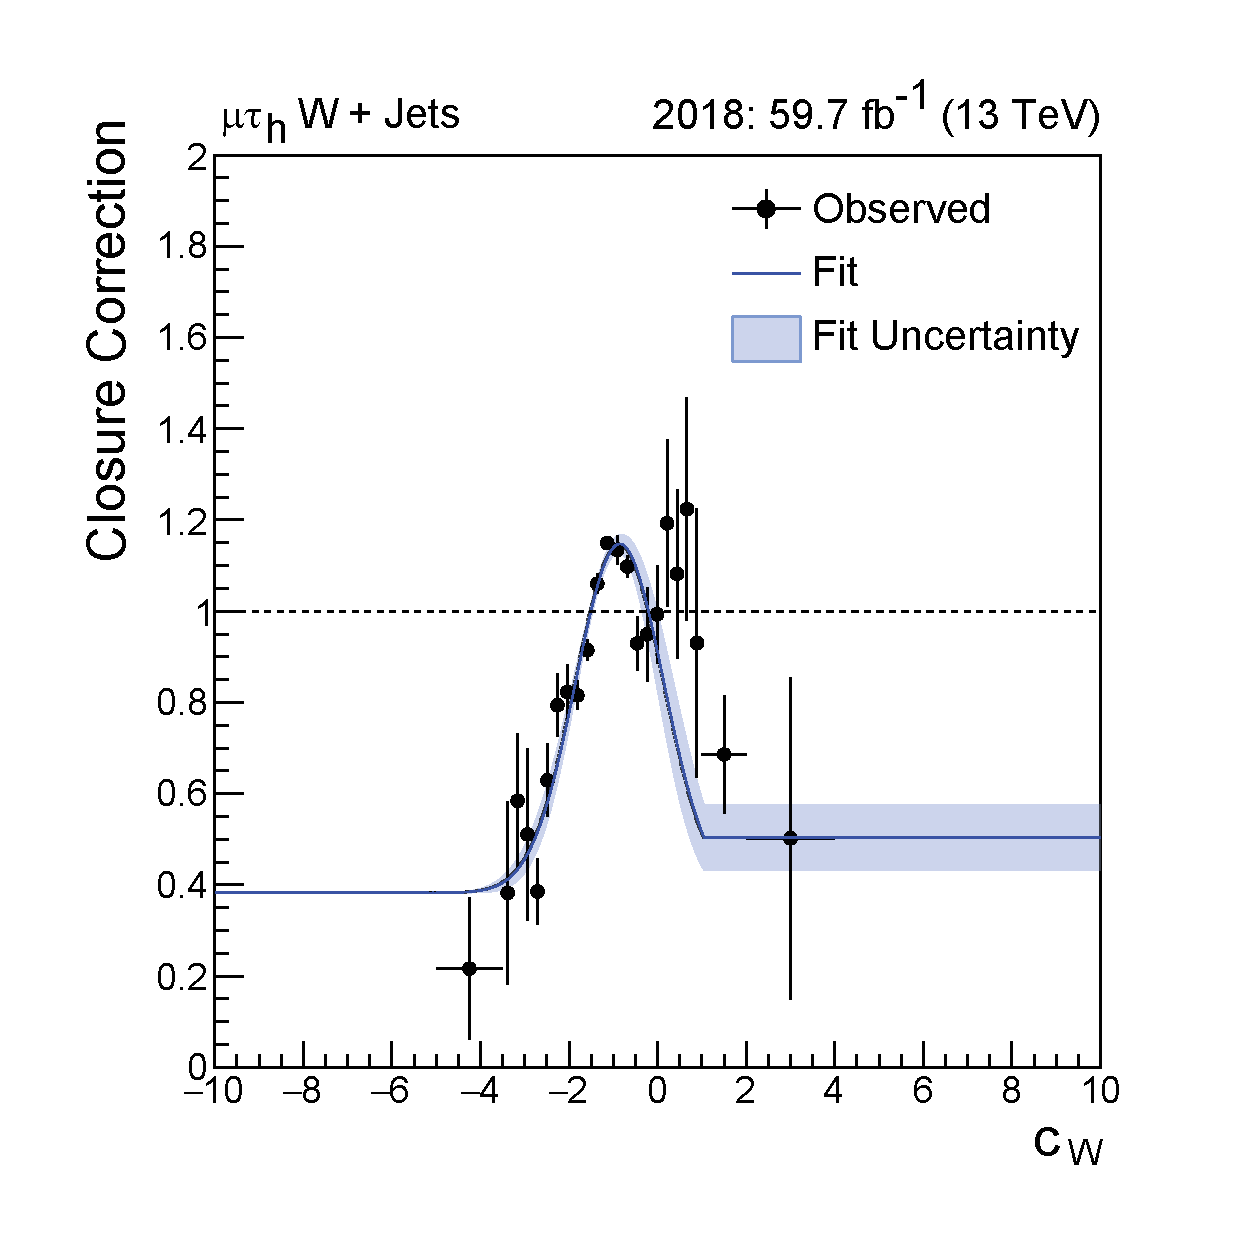
\includegraphics[width=0.33\textwidth]{Figures/ff_closure_met_0jet_closure_wjets_mt_2018-EK.pdf}}
\caption[Plots of fake factor \texttt{Determination Region} closure correction fits.]{\texttt{Determination Region} closure correction fits with 2018 data. (a) is the correction parametrised by $\Delta R$ in events with $N_{\text{b jets}}=0$ in the $\tauhtauh$ channel. (b) and (c) show the correction for the $\mutauh$ channel parametrised by the specific correction variables defined in Equations~\ref{eqn:c_qcd} and \ref{eqn:c_w} for QCD and W + jets processes respectively.}
\label{fig:ff_dr}
\end{figure}

\begin{figure}[!hbtp]
\centering
    \subfloat[]{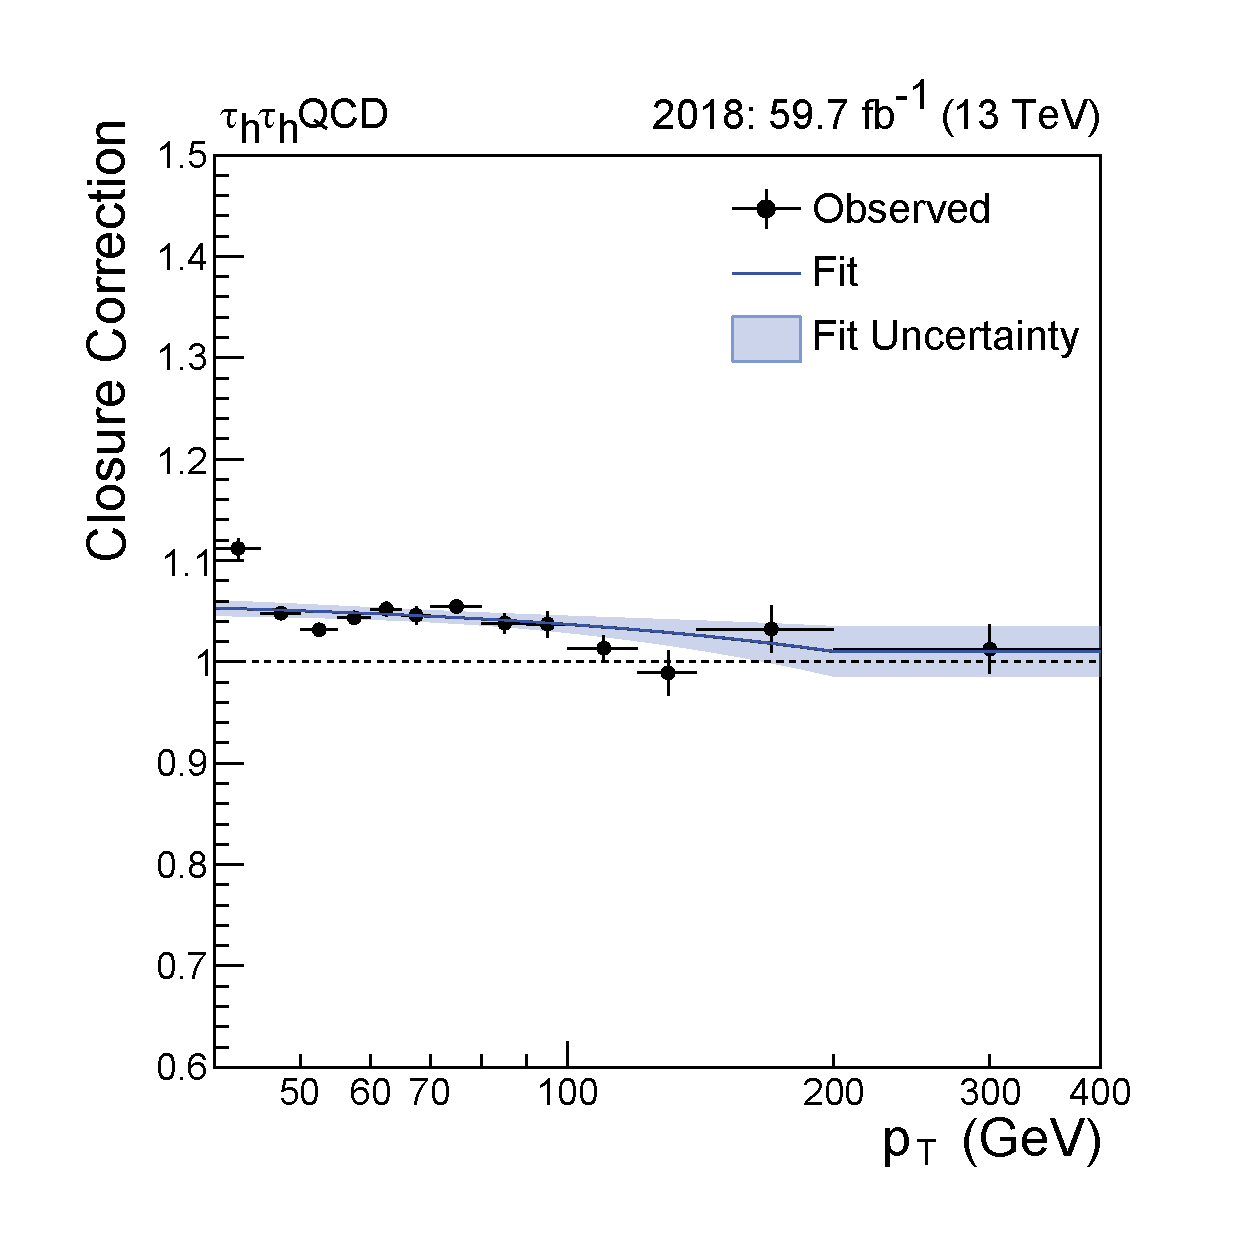
\includegraphics[width=0.33\textwidth]{Figures/ff_closure_os_closure_nbjet0_alt_qcd_tt_2018_v2-EK.pdf}} 
    \subfloat[]{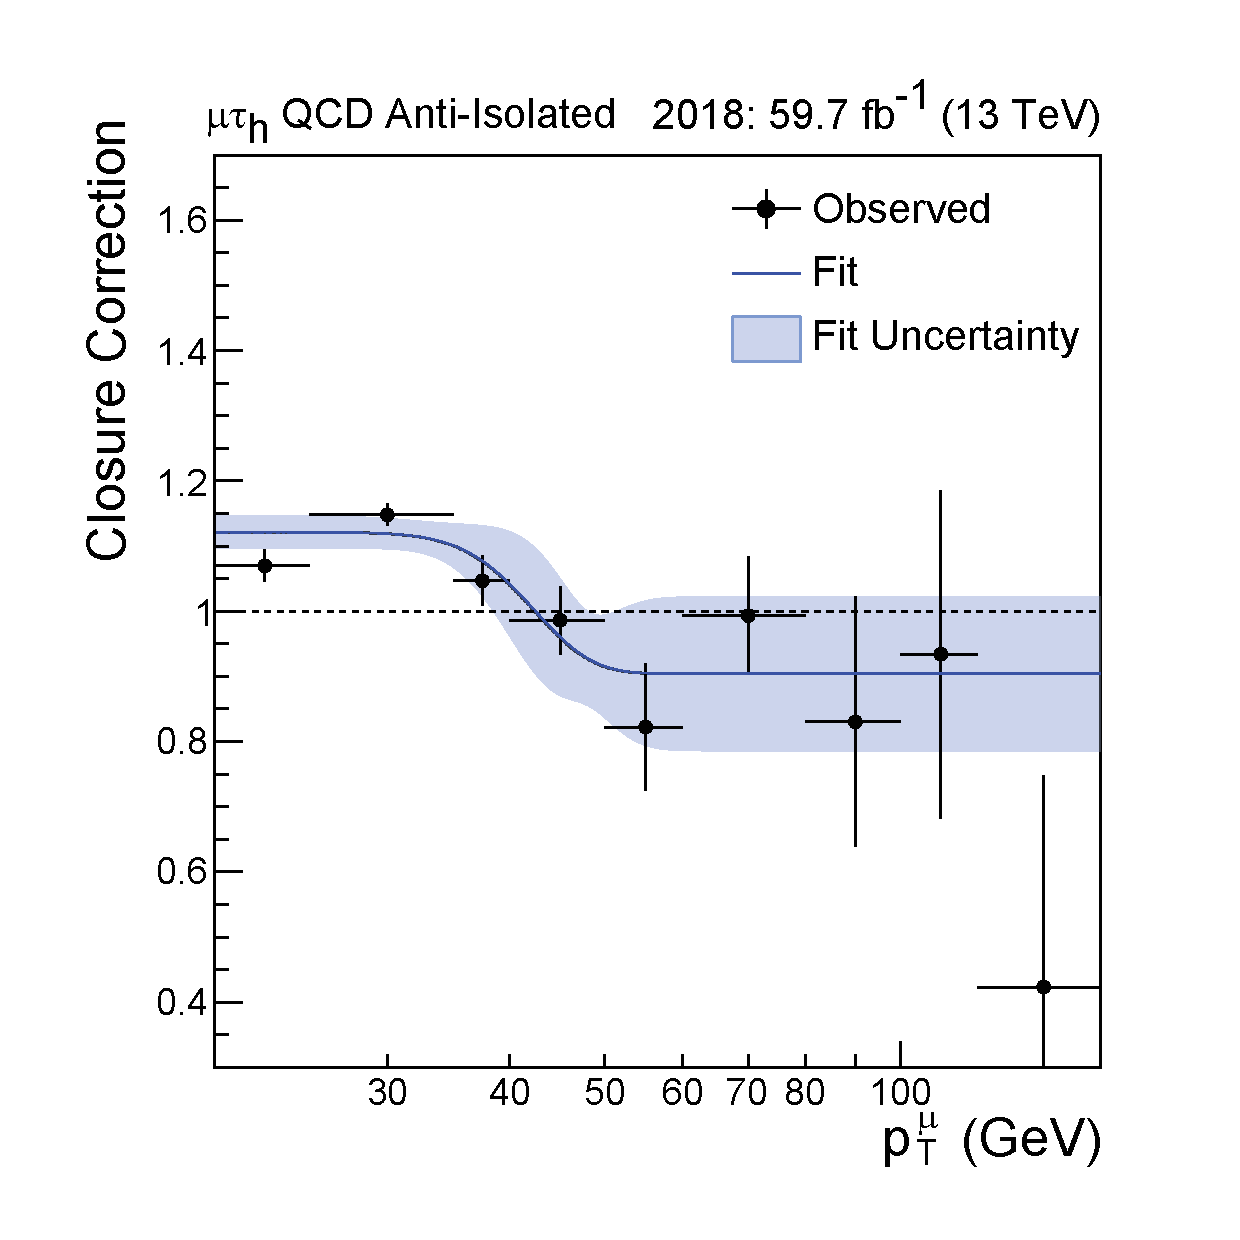
\includegraphics[width=0.33\textwidth]{Figures/ff_closure_pt_1_nbjets0_dr_to_ar_aiso_closure_qcd_mt_2018-EK.pdf}}
    \subfloat[]{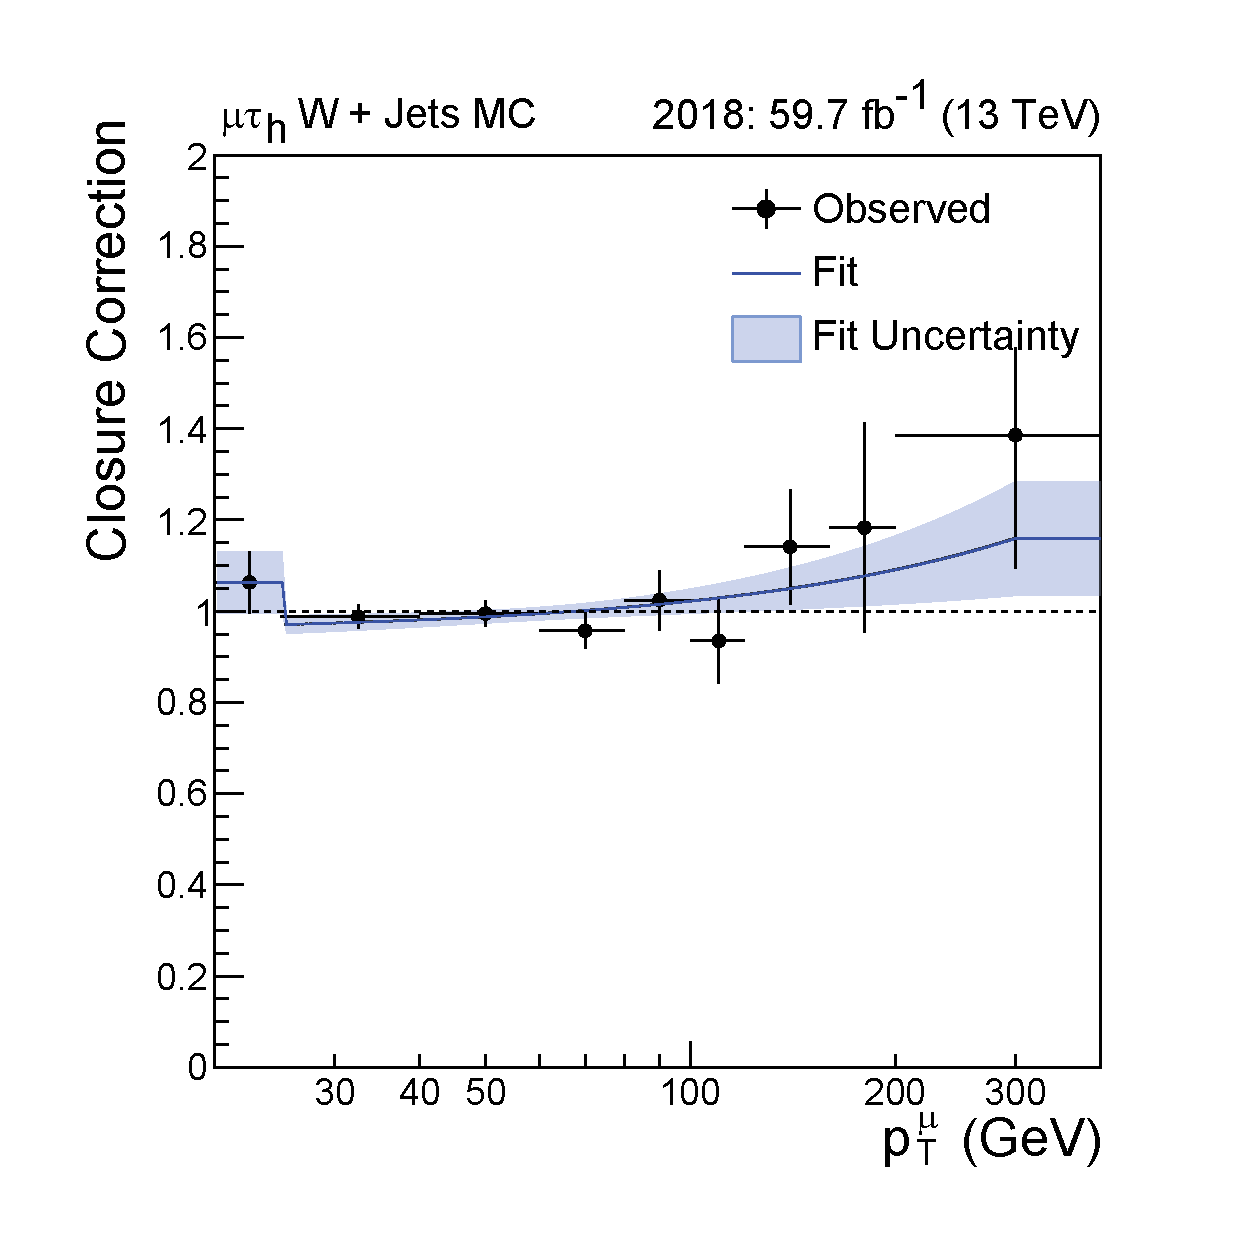
\includegraphics[width=0.33\textwidth]{Figures/ff_closure_pt_1_nbjets0_tightmt_dr_to_ar_closure_wjets_mc_mt_2018-EK.pdf}}
\caption[Plots of fake factor \texttt{Determination Region} to \texttt{Application Region} closure correction fits.]{\texttt{Determination Region} to \texttt{Application Region} closure correction fits with 2018 data. (a) is the correction moving from same sign to opposite sign $\tau$ leptons the parametrised by leading $\tauh$ $\pT$ in events with $N_{\text{b jets}}=0$ in the $\tauhtauh$ channel. (b) and (c) show the correction for the $\mutauh$ channel moving from same sign to opposite sign $\tau$ leptons and high $m_{T}$ to low $m_{T}$ both parametrised by the muon $\pT$ for QCD and W + jets processes respectively.}
\label{fig:ff_dr_to_ar}
\end{figure}

\subsection{Applying fake factors}
\label{sec:ff_applying}

In the $\etauh$ and $\mutauh$ channels, the $\FFi$ measured for the different processes, $i$, are combined into an overall factor $\FF$ using,
\begin{equation}
\FF = \sum_{i}f_{i}\cdot \FFi,
\end{equation}
where the factor $f_{i}$ is defined as,
\begin{equation}
f_{i} = \frac{N_{\text{AR}}^{i}}{\sum\limits_{j}N_{\text{AR}}^{j}},
\end{equation}
which is the fraction of events with a \jtth originating from process $i$ over the total number of \jtth events for all processes in the \texttt{Application Region}.
These fractions of events are estimated with \ac{MC}, with a \ac{QCD} model extrapolated from same sign $\tau$ pairs, and examples are shown in Figure~\ref{fig:mt_ff_frac}.
It is observed that W + jets is the dominating process in this region, however, there are effects from \ac{QCD} at low $\mT$ and from $\ttbar$ in the b-tagged categories. 
These fractions are then multiplied by the relevant corrected $\FF$ and applied to the fail $\tauh$ identification region in C, where this region is purified by subtracting any non \jtth events with \ac{MC}. \\

\begin{figure}[!hbtp]
\centering
    \subfloat[]{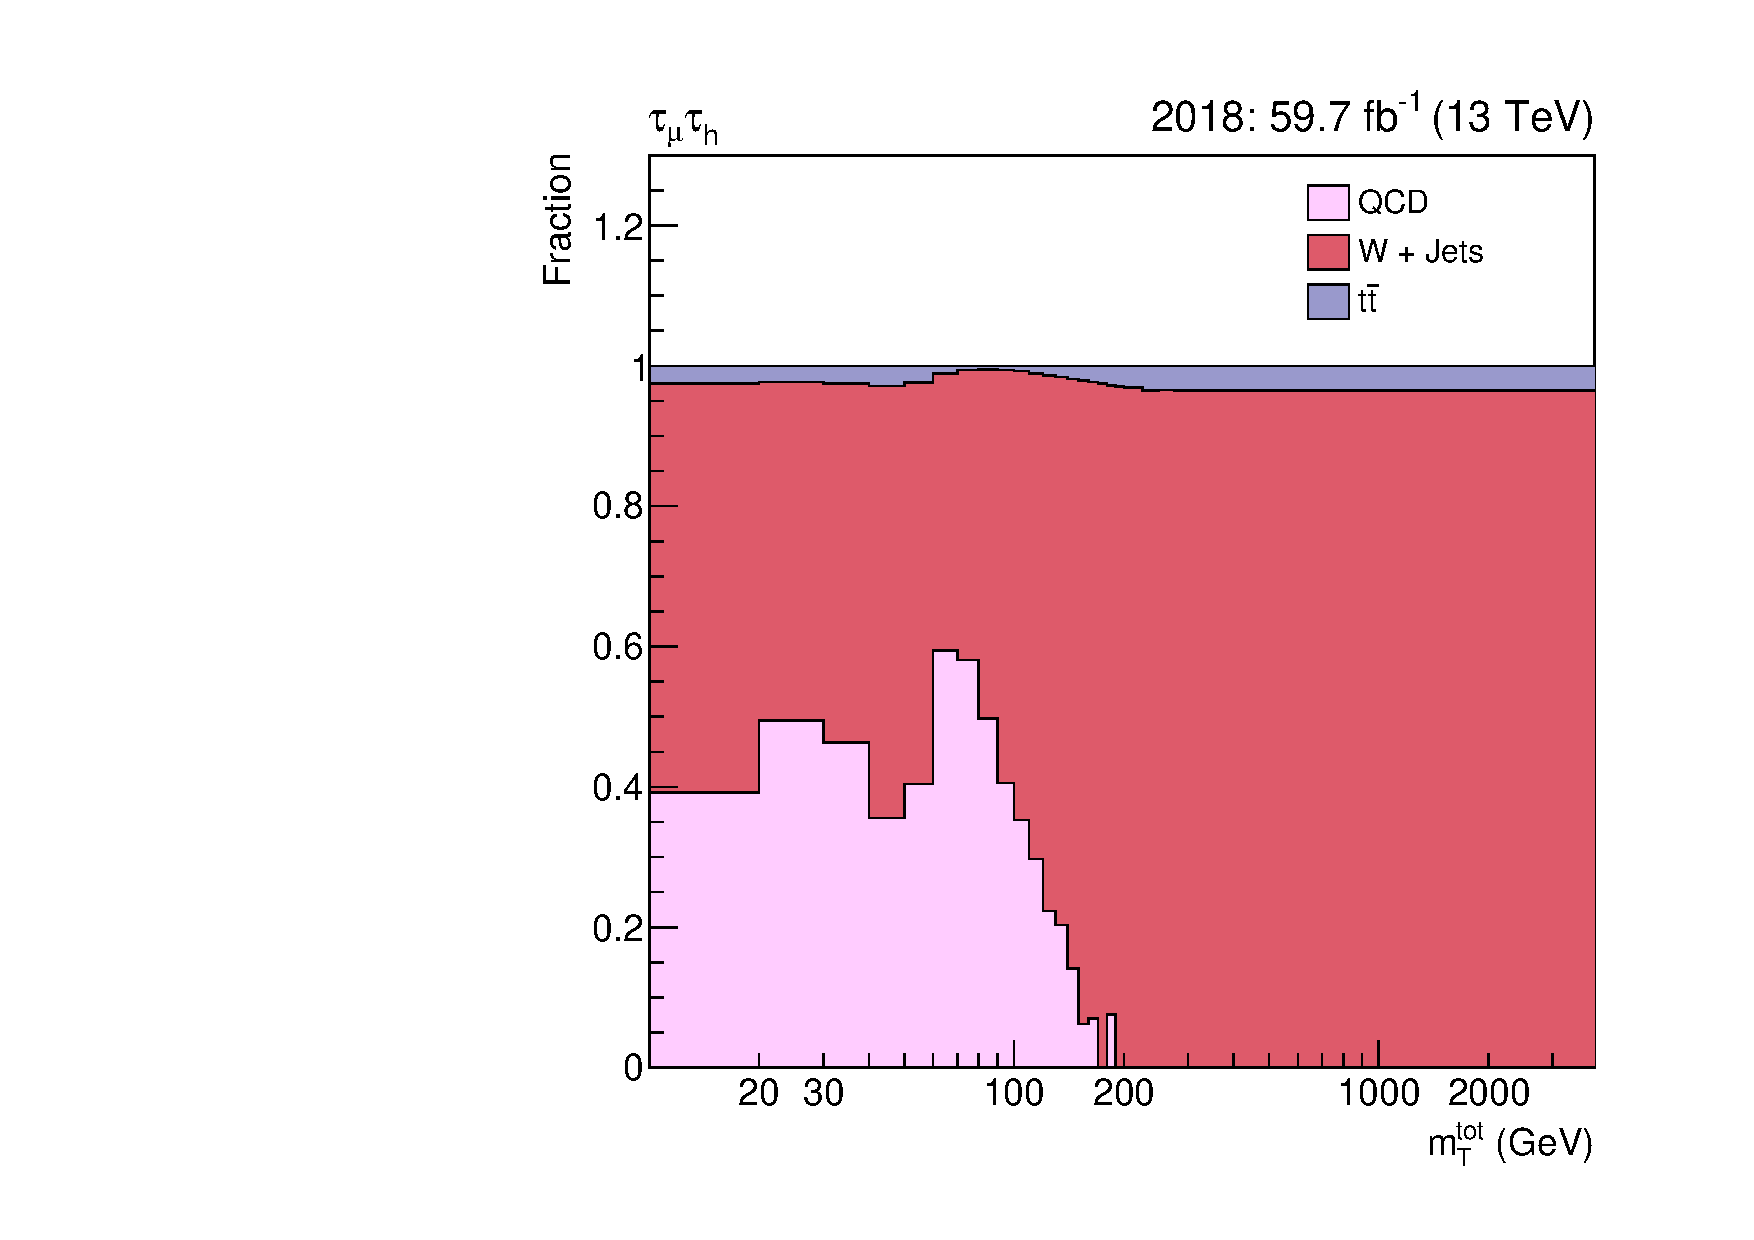
\includegraphics[width=0.45\textwidth]{Figures/ff_fraction_tightmt_nbjets0_mt_2018_os_rebinning.pdf}}
    \subfloat[]{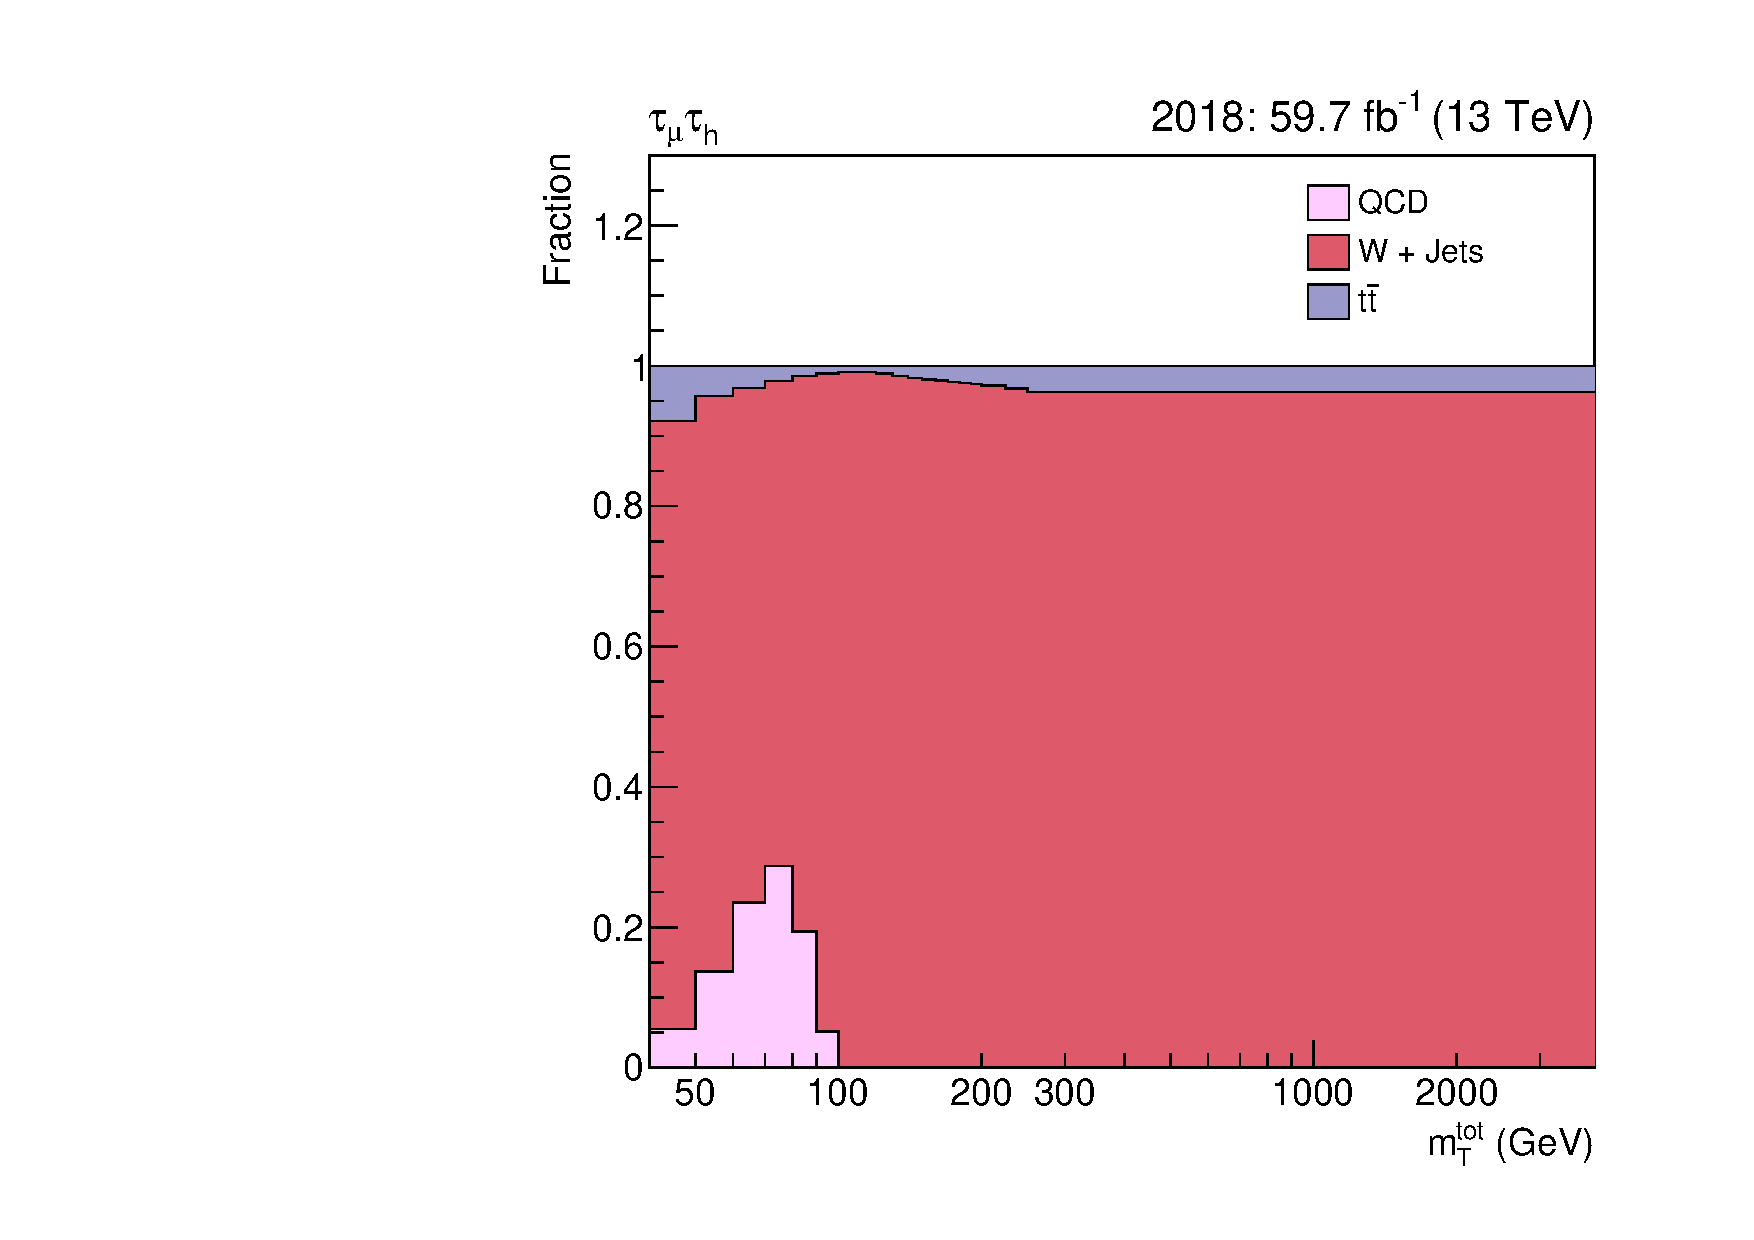
\includegraphics[width=0.45\textwidth]{Figures/ff_fraction_loosemt_nbjets0_mt_2018_os_rebinning.pdf}} \\
    \subfloat[]{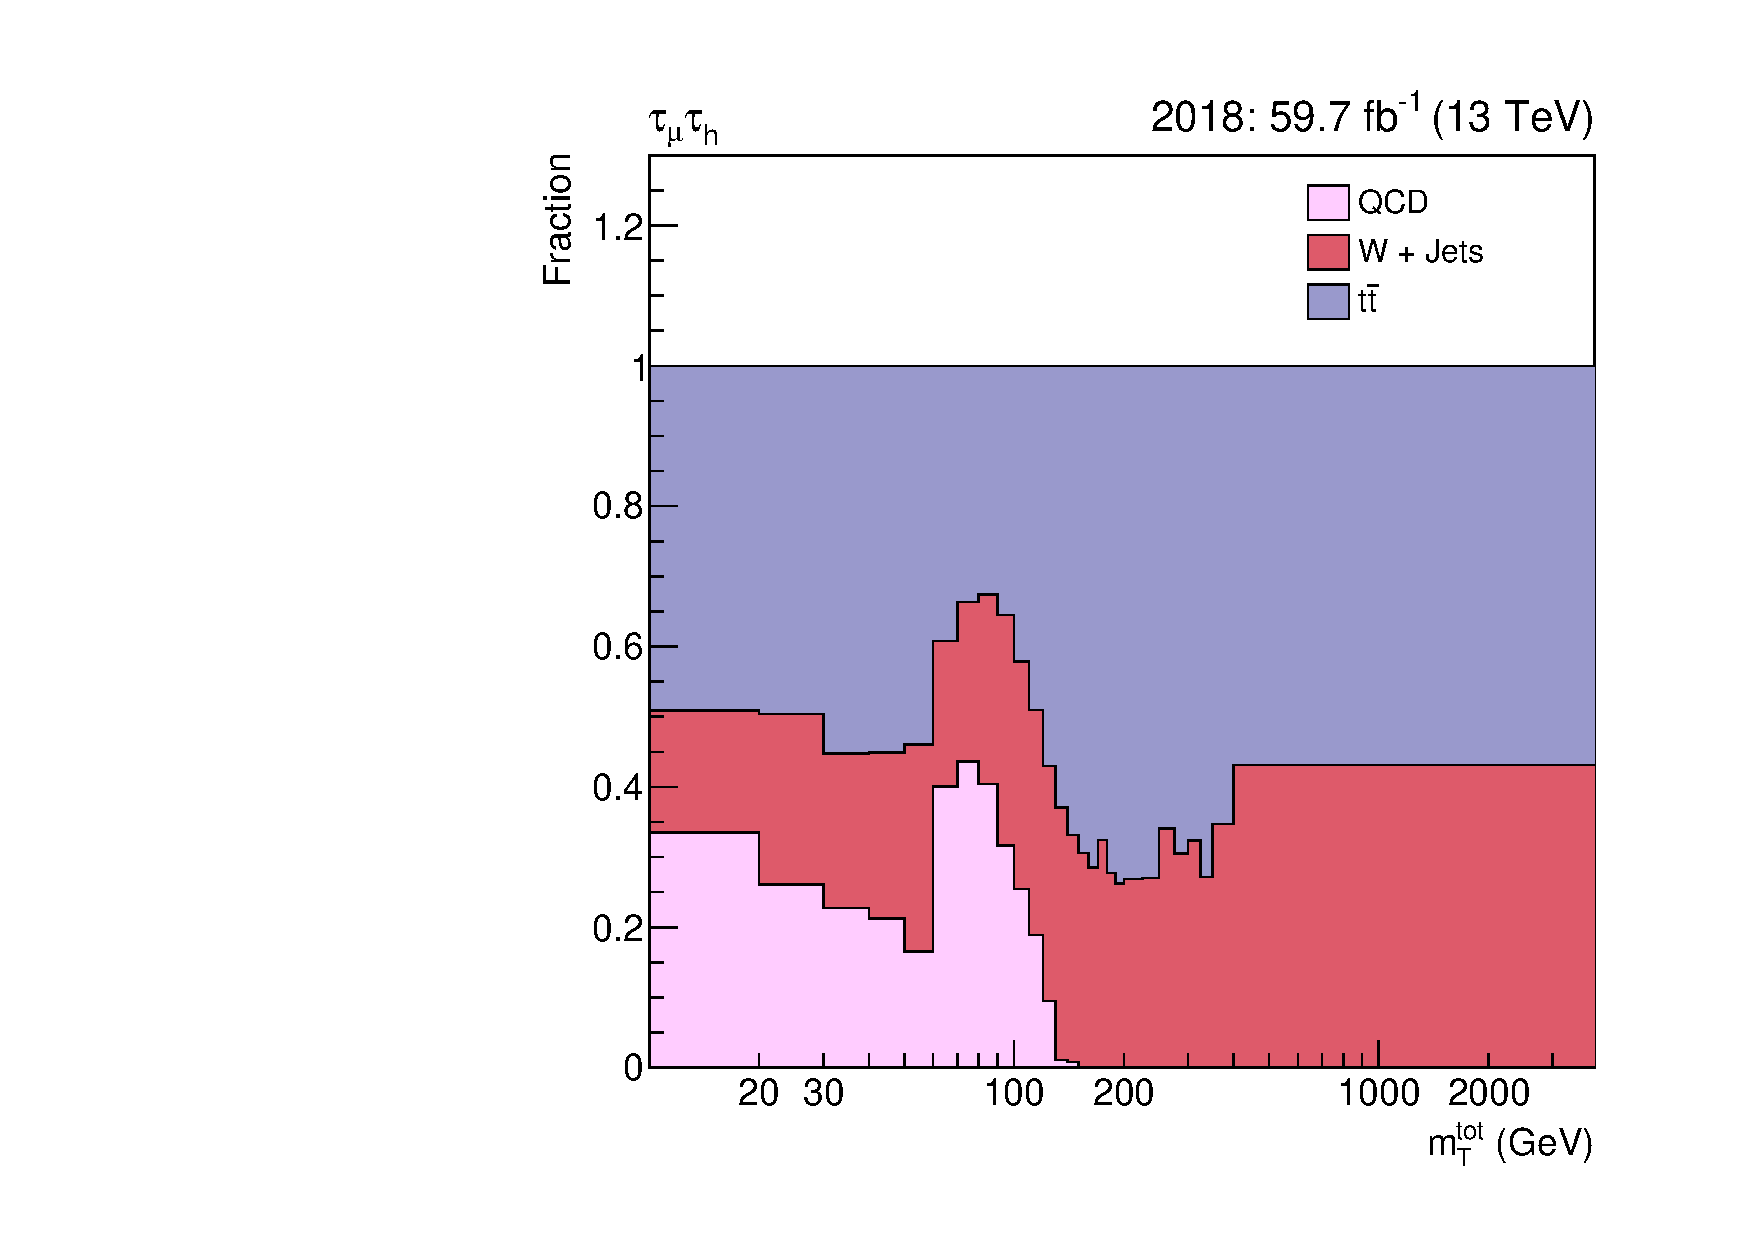
\includegraphics[width=0.45\textwidth]{Figures/ff_fraction_tightmt_nbjets1_mt_2018_os_rebinning.pdf}}
    \subfloat[]{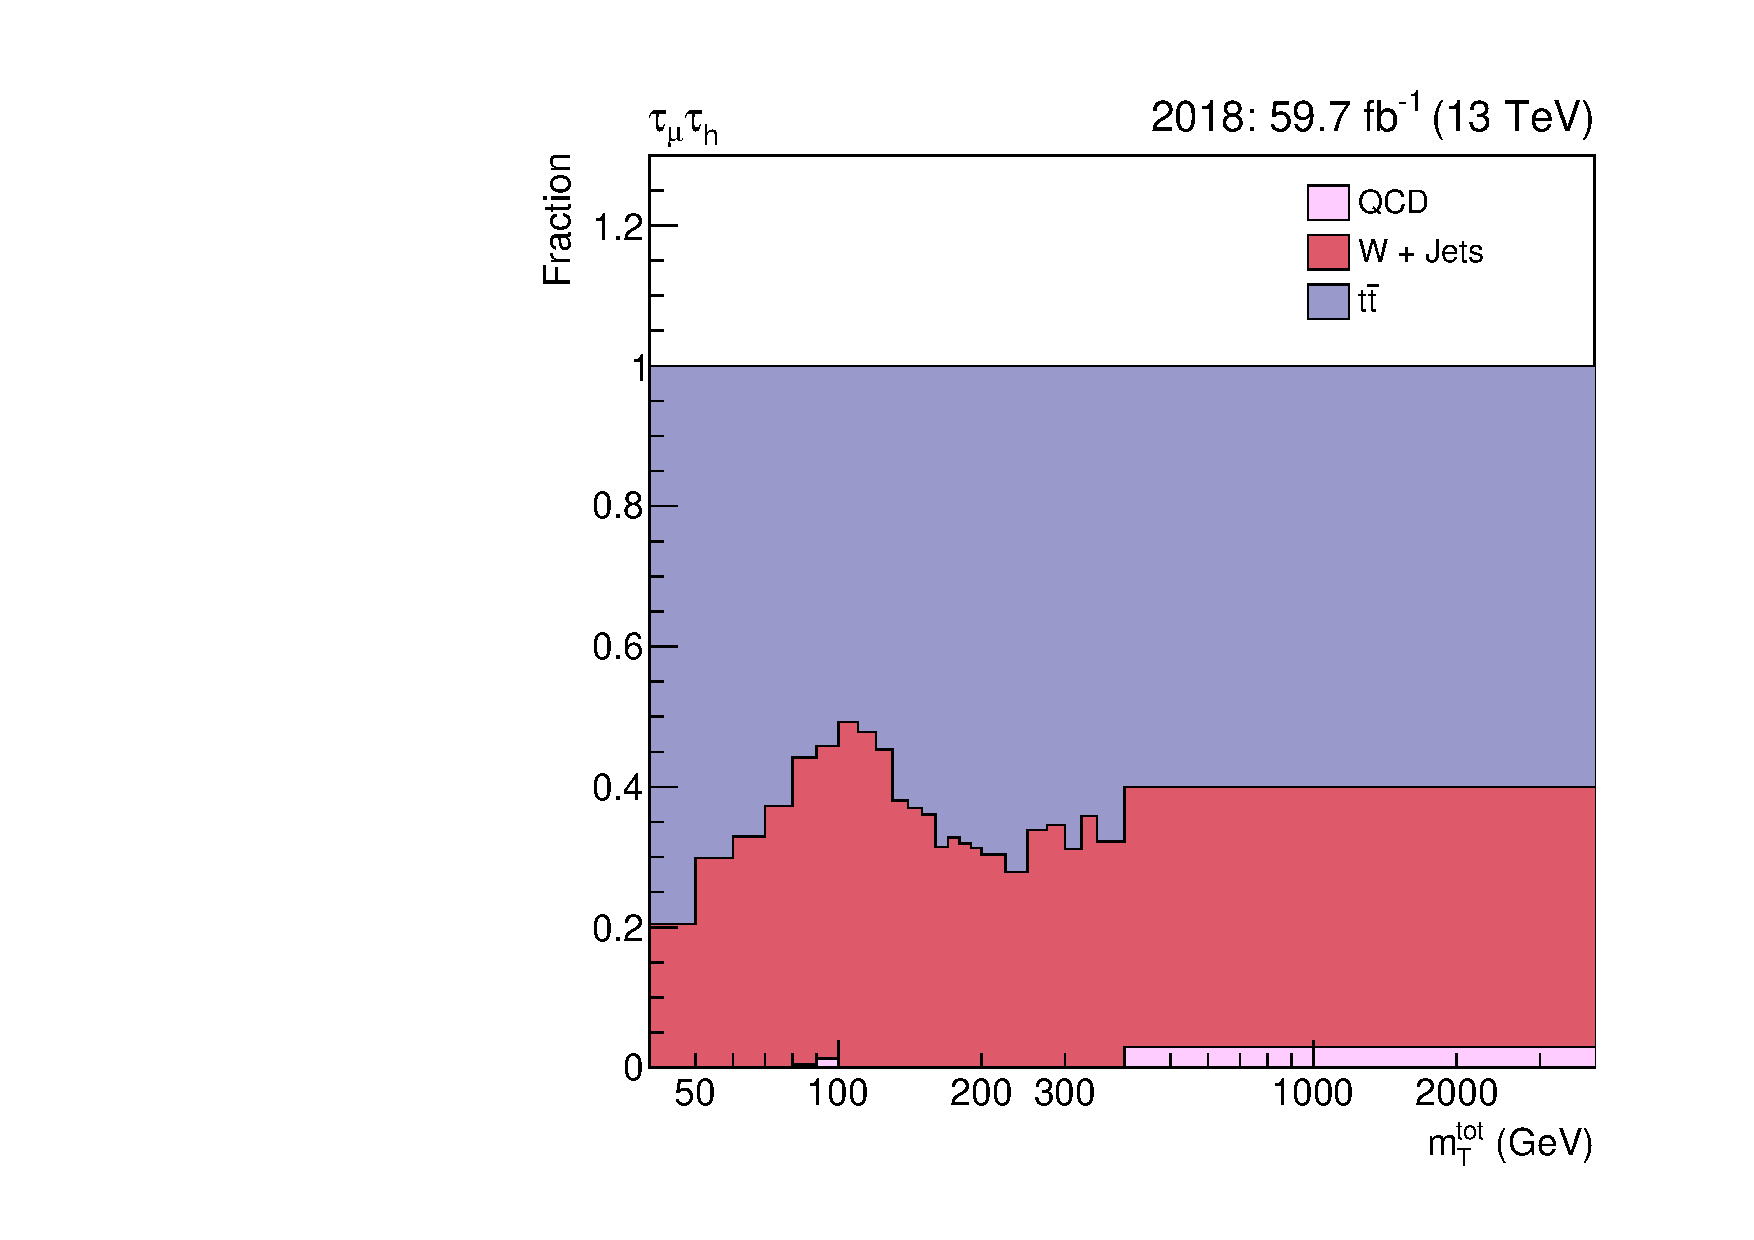
\includegraphics[width=0.45\textwidth]{Figures/ff_fraction_loosemt_nbjets1_mt_2018_os_rebinning.pdf}} \\
\caption[Plots of the expected fake factor \texttt{Application Region} fractions of the processes in the $\mutauh$ channel.]{The expected \texttt{Application Region} fractions of the processes in the $\mutauh$ channel. (a) and (b) show the no b tag \texttt{Tight-$m_{T}$} and \texttt{Loose-$m_{T}$} categories and (c) and (d) show the b tag \texttt{Tight-$m_{T}$} and \texttt{Loose-$m_{T}$} categories respectively.}
\label{fig:mt_ff_frac}
\end{figure}

The $\tauhtauh$ channel has two $\tau_h$ candidates that a jet can be misidentified as.
For this analysis, the $\FF$ are only applied to the leading $\tau_h$ candidate failing the $\tau_h$ identification in C.
This models all events where the leading $\tau_h$ candidate is a \jtth.
However, this leaves a small fraction of events, where the leading candidate is a genuine $\tau$ and the sub-leading candidate is a \jtth.
This contribution (mostly from W + jets) is added back with \ac{MC}.

\section{MC corrections}
\label{sec:ditau_corrections}

The corrections stated in this section apply both to simulated and embedding samples, as the $\tau$ decay is simulated, however, they are derived separately. 
For electrons and muons, corrections are applied to triggers, tracking efficiencies, and identification and isolation requirements.
Using the tag-and-probe method, they are obtained in bins of $\pT$ and $\eta$ of the corresponding lepton, with $Z\rightarrow ee$ and $Z\rightarrow\mu\mu$ events. 
These corrections are generally no more than a few percent. 
The energy scale of the electron is adjusted to the scale measured in data using the Z boson mass peak in $Z\rightarrow ee$ events. 
This effect is negligible in muons. \\

Similarly, corrections are derived for the efficiencies of triggering and identification of $\tauh$ candidates. 
In the $\etauh$ and $\mutauh$ channels, trigger efficiency corrections are obtained from the ratio of fits to data versus simulated samples, for the trigger efficiency as a function of $p_{T}$. 
For the $\tauhtauh$ channel, this is instead done using the binned values of the $\tauh$ decay modes.
The identification efficiency corrections are derived as a function of the $\pT$ of the $\tauh$ candidate. 
Corrections to the energy scale of the $\tauh$ candidates and of electrons misidentified as $\tauh$ candidates are obtained from likelihood scans of discriminating observables, such as the reconstructed $\tauh$ candidate mass. 
For muons misidentified as $\tauh$ candidates, the energy scale correction is negligible. \\

The magnitude and resolution of the \ac{MET} need correcting in embedding events, to take into account the incomplete removal of energy deposits from muons replaced by simulated $\tau$ decays during the embedding procedure. 
These corrections are derived by comparing $\pT^{\text{miss}}$ in embedded events to fully simulated events. \\

In fully simulated events, a specific trigger inefficiency caused by a shift in the timing of the inputs of the \ac{ECAL} L1 trigger in the region at $|\eta|>2.5$ during the 2016 and 2017 data taking~\cite{CMS:2020cmk}, is needed to be corrected.
This effect is named \say{prefiring}.
This resulted in a loss of efficiency for events containing an electron or jet with $\pT$ larger than approximately 50 or 100 GeV, in 2016 and 2017 respectively. 
Corresponding corrections are derived from data and applied to the simulation. \\

Corrections to the energy of jets are calculated in bins of the jet $\pT$ and $\eta$.
These range from subpercent levels in the central part of the detector to a few percent in the forward region. 
The energy resolution of the simulated jets is also tuned to match that of the data. 
A correction is applied to the missing transverse momentum, based on differences in the estimated hadronic recoil between data and simulation. 
An \ac{MC} to data correction for a b jet passing the selection criteria is also determined. 
This correction can alter the number of b jets in a simulated event. \\

Any differences from simulated events to data, where an electron or muon is reconstructed as a $\tauh$, are corrected from the pure $Z\rightarrow ee$ and $Z\rightarrow\mu\mu$ regions. 
Similarly, a correction is applied to account for residual differences in the $\mu\rightarrow e$ misidentification rate between data and simulation. \\

Further \ac{MC} to data corrections are applied to the di-lepton mass and $\pT$ spectra in simulated $Z\rightarrow \ell\ell$ events. 
These are derived from $Z\rightarrow\mu\mu$ events.
Additionally, all simulated $\ttbar$ events are weighted to match the t quark $\pT$ distribution observed in data~\cite{CMS:2015rld}.

\section{Uncertainty model}
\label{sec:uncerts}

The statistical uncertainties are taken into account by the Barlow-Beeston method, described in References~\cite{Barlow:1993dm,Conway:2011in}.
The systematic model is split into uncertainties based on the online and offline reconstruction of objects and the background and signal modelling.
An uncertainty is correlated across channels when it represents a shift in the reconstruction of an object and is decorrelated otherwise.
It is decorrelated across the eras of data taking when the shift is derived independently by era.
The embedded samples use the same uncertainty scheme as \ac{MC} but 50\% are correlated and 50\% are uncorrelated with \ac{MC} uncertainties, because of the shared real data in the measurement.

\subsubsection{Hadronic taus}
Uncertainties on the $\tau_h$ triggers are obtained from the fitted scale factors used to derive the corrections for the $\tauh$ trigger efficiencies.
The legs of the double-$\tau_h$ and e/$\mu$-$\tauh$ cross triggers in different decay mode bins are treated as uncorrelated.
For the single-$\tau_h$ trigger leg, due to limited statistics, it is not possible to determine scale factors and uncertainties split by decay mode and therefore a single uncertainty common to all decay modes is applied.
The double-$\tau_h$ trigger uncertainties are further split into the $\pT$ regions $<$ 100 GeV and $>$ 100 GeV to allow the fit more freedom to adjust the high $\pT$ regions relative to the low $\pT$ regions.
Uncertainties are also applied on the energy scale of the $\tau_h$ candidates. 
These uncertainties range between 0.2-1.1\%. 
Finally, an uncertainty on the identification efficiency is placed as a function of $\pT$ in the $\etauh$ and $\mutauh$ channels, and of the $\tauh$ decay mode in the $\tauhtauh$ channels. 
This varies between 3-9\% and is uncorrelated in each variable bin it is derived in.
To account for the different anti-lepton discriminator working points, an uncertainty of 3\% per $\tau_h$ is applied and treated as uncorrelated between the channels where different $D_{\text{WP}}^{e/\mu}$ are used.

\subsubsection{Light leptons}
The uncertainty on the trigger efficiencies amounts to 2\% per lepton in the $\etauh$, $\mutauh$ and $\emu$ channels.
They are normalisation uncertainties but implemented as shape uncertainties as they only touch the events triggered by the corresponding cross-trigger or single lepton triggers.
Uncertainties are also placed on the electron energy scale based on the calibration of \ac{ECAL} crystals.
This information is not reliable for embedding samples and so uncertainties of 0.5-1.25\% are placed here. 
The energy scale variations are negligible and so are not included.
Another 2\% uncertainty is placed on the identification of any electron or muon in the event.

\subsubsection{Jets}
Jet energy scale and resolution uncertainties arise from several sources. 
These include limited statistical measurements used for calibration, energy measurement changes due to detector ageing, and bias corrections to address differences between simulation and data. 
Uncertainty ranges are from subpercent to $\mathcal{O}(10\%)$.
Uncertainties are also placed on the tagging of b jets, which vary from 0--3\%.

\subsubsection{Leptons misidentified as hadronic taus}
Uncertainty shifts are applied for the energy scale of leptons misidentified as $\tauh$ candidates parametrised by the $\pT$ of the e/$\mu\rightarrow\tauh$ fake.
The magnitude is 1.0\% for muons in all eras. 
For electrons the uncertainties vary between 0.5 and 6.6 \%.

\subsubsection{Jets misidentified as hadronic taus}
The backgrounds with jets misidentified as $\tauh$ are estimated from data with the fake factor method. 
There are different sources of uncertainty related to this method.
The first uncertainties come from subtracting off other background processes with \ac{MC} to form the determination region. 
The subtraction is shifted up and down by 10\% to determine new weights.
Next, statistical uncertainties on all of the fake factor method fits are accounted for, where the binned values are uncorrelated with the rest of the fit.
An uncertainty is also placed on the choice of fit function, which is calculated by comparing the fits to a first-order polynomial fit set to constant above 100 GeV.
The final systematic variation is on the \texttt{Determination Region} to \texttt{Application Region} corrections by applying them twice and not at all to get symmetric shifts.
The size of each systematic uncertainty varies from 0--10\%, whilst the statistical element from the fits can be larger in the tails of the distributions.

\subsubsection{Jets misidentified as light leptons}
Backgrounds with jets misidentified as electrons or muons from \ac{QCD} are only considered in the $\emu$ channel and modelled from data.
Uncertainties are placed based on the statistical uncertainties in the determination region which are 2--4\% and the extrapolations to the signal region that are $\mathcal{O}(10\%)$.

\subsubsection{Muons misidentified as electrons}
Backgrounds with muons misidentified as electrons are only considered in the $\emu$ channel.
These events are modelled from \ac{MC} and any generator-matched muon identified as an electron is given a 15\%--45\% uncertainty, which is derived from the calculation of the correction.

\subsubsection{MET}
The \ac{MET} uncertainties are different depending on the process.
For all processes that are not $\ttbar$ or di-boson, the hadronic recoil response and its resolution are varied within the uncertainties determined during the computation of the recoil corrections.
For $\ttbar$ or di-boson an uncertainty is derived from the energy carried by an unclustered particle~\cite{Sirunyan:2019kia}.
These uncertainties vary between 0--10\%.

\subsubsection{Background process-specific uncertainties}
Uncertainties on the $\ttbar$ $\pT$ and Z boson $m_{\ell\ell}$-$\pT$ reweighting are placed by applying the correction twice and not at all.
An additional uncertainty is placed to cover the $\ttbar$ contamination in embedding, where the removed $t\bar{t}$ genuine $\tau$ pair is shifted up and down by 10\%.
Some non-closures are observed in embedded $Z\to\mu\mu$ control samples. 
Therefore, these non-closures are taken as an additional shape uncertainty as a function of the Z $\pT$ and $m_{\tau\tau}$.
Uncertainties on the normalisation background processes with sizes 4\% for $Z\rightarrow ll$ and W + jets production~\cite{Melnikov:2006kv}, 6\% for $\ttbar$ production~\cite{Czakon:2011xx,Kidonakis:2013zqa}, and 5\% for diboson and single t quark production~\cite{Kidonakis:2013zqa,Campbell:2011bn,Gehrmann:2014fva}.

\subsubsection{Signal process specific uncertainties}
For the gg$\phi$ and bb$\phi$ processes, the variation of the \texttt{hdamp} parameter of the \POWHEG \ac{MC} generator as well as the $\mu_{R}$/$\mu_{F}$ scale variations are used to determine the uncertainties on the $\pT$ spectrum of each contribution at NLO QCD to the Higgs boson production via gluon fusion (t-only, b-only, tb-interference). 
These are also determined from additional samples produced at generator level and applied as event weights depending on $\pT$ after the parton shower simulation.
For the vector leptoquark signal samples, the parton distribution functions and $\mu_{R}$/$\mu_{F}$ scale variations are applied on an event-by-event basis.
These uncertainties are included as shape uncertainties as they may affect the shapes of the $m_{T}^{\text{tot}}$ distribution as well as the predicted signal yields.

\subsubsection{Luminosity}
$1.2\%$, $2.3\%$ and $2.5\%$ normalisation uncertainties for the luminosity are applied to the 2016, 2017 and 2018 templates respectively, which originate from MC simulation to data comparisons.

\subsubsection{Prefiring}
Upper and lower bounds are taken from the efficiency maps and propagated to all \ac{MC} samples as shape uncertainty for 2016 and 2017.
The size of the uncertainty depends on the event topology but averages to a value of the order of 1\%.

\section{Signal extraction}
\label{sec:sig_ext}

A simultaneous binned maximum likelihood fit over all analysis categories is used to extract the results.
The likelihood takes the form,
\begin{equation}
\mathcal{L}(\text{data}\mid\mu,\theta) = \prod_{i}^{N_{i}} \text{Poisson} \Big(n_{i} \mid \sum_{j}^{N_{j}} g_{j}(\mu_{ij}) \cdot s_{ij}(\theta) + \sum_{k}^{N_{k}} b_{ik}(\theta)\Big) \cdot p(\hat{\theta} \mid \theta),
\label{eqn:likelihood}
\end{equation}

where $i$ loops through all histogram bins and analysis categories.
The indices $j$ and $k$ loop over all signal and background processes for the hypothesis being fit.
$n_i$, $s_i$ and $b_i$ are the data observed, signal and background expectation respectively in each bin.
$\theta$ represents the set of nuisance parameters (corresponding to the systematic uncertainties as detailed in Section~\ref{sec:uncerts}) that parametrise the signal and background modelling.
$\mu$ are rate parameters and $g(\mu)$ are scaling functions that scale a signal to a specific hypothesis.
The form of the Poisson probabilities are,
\begin{equation}
\text{Poisson} (n \mid x) = \frac{x^{n}e^{-x}}{n!}.
\end{equation}
Finally, $p(\hat{\theta} \mid \theta)$ represents the \ac{PDF} of each nuisance parameter ($\theta$) with respect to the initial value of the parameter ($\hat{\theta}$). \\

The \ac{PDF}s come in two forms, the first is for uncertainties that only affect the normalisation of the process and are modelled by log-normal \ac{PDF}s. 
The second is for uncertainties that affect the shape of the distribution, these are assigned Gaussian \ac{PDF}s.
The $\pm1\sigma$ shifts for each shape variation are derived and vertical morphing~\cite{Conway:2011in} is used to interpolate and extrapolate within and outside the shifts.
Both \ac{PDF}s are dependent on the mean ($\mu$) and standard deviations ($\sigma$) and the functional forms are shown in Table~\ref{tab:pdfs}. \\

\begin{table}[!hbtp]
    \centering
    \begin{tabular}{|c|c|}
         \hline
         Gaussian & Log-normal  \\
         \hline
         \hline
          & \\
         $f(x) = \frac{1}{\sqrt{2\pi\sigma^{2}}} \exp\Big({-\frac{(x - \mu)^2}{2\sigma^2}}\Big)$ & $f(x) = \frac{1}{x} \frac{1}{\sqrt{2\pi\sigma^{2}}} \exp\Big({-\frac{(\ln x - \mu)^2}{2\sigma^2}}\Big)$ \\
          & \\
         \hline
    \end{tabular}
    \caption[PDFs used for nuisance parameters.]{Table of PDFs used for nuisance parameters.}
    \label{tab:pdfs}
\end{table}

The following subsections discuss the results of many such fits.
The key fits to understand the results are the background-only fit and the signal-plus-background fits.
The background-only fit is performed with $N_j$ (number of signal processes) set to 0.
For all signal-plus-background fits, the fit is done to a single mass hypothesis, however, within this mass hypothesis there can be a number of signal processes.
The model-independent resonance search has separate gg$\phi$ and bb$\phi$ signal modes and so two rate parameters $\mu_{\text{gg}\phi}$ and $\mu_{\text{bb}\phi}$ are needed.
The samples are initially scaled to the cross-section times branching ratio ($\sigma \times B (\phi\rightarrow\tau\tau)$) of 1 pb.
Setting $g(\mu)=\mu$ for both processes, $\mu_{\text{gg}\phi}$ and $\mu_{\text{bb}\phi}$ represent the $\sigma \times B (\phi\rightarrow\tau\tau)$ in units of pb.
To avoid negative signal strengths, $\mu$ is not allowed to become negative.
Also used in the following subsections, is a signal-plus-background channel/category compatibility fit.
In this fit, the signal processes and rate parameters are further split into each channel or category utilising index $i$ in Equation~\ref{eqn:likelihood}.
This is used to determine the compatibility of the results in different decay channels and analysis categories.
In this case, $\mu$ is allowed to take negative values to help fully understand the fits to data in each channel or category. \\

The vector leptoquark search has two signal modes: the t-channel interaction and the interference with $Z/\gamma^* \rightarrow \tau\tau$. 
However, as this is a model-dependent interpretation of these results both these rate parameters scale together.
The scaling functions differ between the two processes with $g_{\text{t-channel}}(\mu) = \mu^4$ and $g_{\text{interference}}(\mu) = \mu^2$ to mimic how the cross-sections of each process scale.
When the initial samples are scaled to the cross-section at $g_{U}=1$, $\mu$ corresponds to the coupling $g_{U}$. \\

For the \ac{MSSM} interpretation of the results, there are three Higgs bosons to consider in the signal model (h, H and A) produced via both gluon fusion and in association with b quarks.
The gg$\phi$ samples are also split into separate loop contributors, so the kinematic properties can be properly scaled to \ac{MSSM} prediction, as described in Section~\ref{sec:additional_higgs_bosons}.
The \ac{SM}-like Higgs boson is considered in the \ac{MSSM} signal model to monitor differences in the observed Higgs boson prediction between the \ac{MSSM} and the \ac{SM}.
In each benchmark scenario chosen, the signal prediction depends only on $m_{A}$ and $\tan\beta$ and the scaling to cross-section is shown in Equation~\ref{eqn:mssm_xs}.
As the potential scaling functions for \ac{MSSM} interpretations are not necessarily smooth one-to-one mappings, the likelihood is tested for individual points on the $m_{A}$-$\tan\beta$ parameter space.
At each point, the \ac{MSSM} Higgs bosons are scaled to the theory predicted cross-section times branching ratio.
To test the \ac{MSSM} hypothesis over the \ac{SM} hypothesis, the single rate parameter $\mu$ is used and only allowed to take values of 1 (\ac{MSSM}) and 0 (\ac{SM}) with $g(\mu)=\mu$.
As the SM Higgs boson is added to the background modelling and the \ac{MSSM} prediction of the observed Higgs boson is added to the signal model when $\mu=1$, the \ac{SM} Higgs boson prediction must then be subtracted from the signal model. \\

The confidence intervals in the best-fit results are given by the $-2\Delta\ln\mathcal{L}$, where $\Delta\ln\mathcal{L}$ is the difference between $\ln\mathcal{L}$ of the best-fit model and the test value of $\mu$. 
The 68\% and 95\% \ac{CL} regions with two degrees of freedom (as in the model-independent resonant search) are determined by $-2\Delta\ln\mathcal{L} = 2.28$ and $5.99$ respectively. \\

Upper limits are placed using the modified frequentist approach~\cite{Junk:1999kv,Read:2002hq} with a profile likelihood ratio used for the test statistic, as defined below.
\begin{equation}
  q_{\mu} = -2 \ln \Biggl(\frac{\mathcal{L}(\text{data} | \mu, \hat{\theta}_{\mu})}{\mathcal{L}(\text{data} | \hat{\mu}, \hat{\theta}_{\hat{\mu}})}\Biggl), 0 \leq \hat{\mu} \leq \mu,
\end{equation}
where $\hat{\mu}$ and $\hat{\theta}_{\hat{\mu}}$ are the best fit values of $\mu$ and $\theta_\mu$. 
$\hat{\theta}_{\mu}$ are the values of $\theta_\mu$ that are maximised by the likelihood for a tested value of $\mu$.
The bounds on $\hat{\mu}$ are to ensure a positive signal strength with a one-sided confidence interval.
The probability of $q_{\mu} \geq q_{\mu}^{\text{obs}}$ is,
\begin{equation}
\text{CL}(\mu) = \int^{\infty}_{q_{\mu}^{\text{obs}}} f(q_{\mu} \mid \mu, \theta_{\mu}^{\text{obs}}),
\end{equation}
where $f(q_{\mu} \mid \mu, \theta_{\mu}^{\text{obs}})$ is the \ac{PDF} of $q_\mu$.
$\text{CL}_{b}$ and $\text{CL}_{s+b}$ are then defined by the relevant background-only and signal-plus-background fits.
$\text{CL}_s$ is defined as the ratio of $\text{CL}_{s+b}$ and $\text{CL}_{b}$ and then upper limits are placed at the confidence level of $1-\text{CL}_{s}$.
The $f(q_{\mu} \mid \mu, \theta_{\mu}^{\text{obs}})$ are determined using the asymptotic approximation \cite{Cowan:2010js} and results are cross-checked and deemed consistent with toy MC datasets. \\

If a deviation from the background expectation is observed, the size of the deviation is quantified by significance.
To test the rejection of the background-only hypothesis in favour of the signal-plus-background hypothesis, $\mu$ is replaced with 0 in the test statistic.
The $p$-value, $p_0$ is then,
\begin{equation}
p_{0} = \int^{\infty}_{q_{0}^{\text{obs}}} f(q_{0} \mid 0, \theta_{\mu}^{\text{obs}}).
\end{equation}
$p_{0}$ is uniformly distributed between 0 and 1 for the background-only hypothesis and so the probability and significance of rejecting the background-only hypothesis can be found. \\

\section{Postfit plots}

Figures~\ref{fig:low_mass_postfit} and \ref{fig:high_mass_postfit} show the unblinded distributions in the most sensitive analysis categories.
For simplicity, the $\etauh$ and $\mutauh$ channels have been combined.
Figure~\ref{fig:low_mass_postfit} shows the distributions of the $m_{\tau\tau}$ discriminator in the no b tag low-mass optimisation categories. 
A signal-plus-background fit for a model-independent gluon fusion resonant mass hypothesis of 100 GeV is shown and the changes in the background modelling when using a background-only fit are displayed in the ratio.
Figure~\ref{fig:high_mass_postfit} shows the distributions of the $m_{T}^{\text{tot}}$ discriminator in the high-mass optimisation categories.
A background-only fit is shown for the stacked background and example signal hypotheses for the model-independent 1.2 TeV gg$\phi$ and bb$\phi$ resonances and 1 TeV VLQ BM 1 mass points are displayed. \\

In the low-mass optimisation categories, a small excess of events is observed on the Z boson peak in the no b tag categories and reasonable agreement is observed in the b tag categories.
The excess of events are distributed in $m_{\tau\tau}$ between 80 and 120 GeV.
A signal-plus-background hypothesis is best fit with a 100 GeV gg$\phi$ signal with a cross-section times branching ratio of 5.8 pb. 
In this same fit, the bb$\phi$ process is constrained by the b tag categories to give a signal yield of 0.
A background-only fit is also performed on the data, it is observed that this can only partly explain the differences observed between background and data.
Even after a background-only fit, there is still a small excess of data events over the Z boson peak. \\

In the high-mass optimisation categories, another small excess is observed in the high $m_{T}^{\text{tot}}$ bins, particularly in the most sensitive no b tag categories.
This excess is best fit by a model-independent gluon fusion resonant mass at 1.2 TeV with a cross-section times branching ratio of 3.1 fb.
There are no considerable differences observed in background modelling between signal-plus-background and background-only fits.
This is because the uncertainties in these bins are more statistically dominated and the majority of the systematic uncertainties are constrained in the bulk of the distribution.
Good agreement is observed in the rest of the distribution.
There is a very small deviation in the b tag categories, but as this can also be explained by a gg$\phi$ signal, the bb$\phi$ signal is heavily constrained and so largely does not contribute to the signal-plus-background fit of the excess.
Similar to the bb$\phi$ signal, the VLQ BM 1 signal is constrained by the results in the b tag categories, leading to a small non-zero best-fit signal strength, but cannot explain the excess in the no b tag categories. \\

\begin{figure}[!hbtp]
\centering
    \subfloat[]{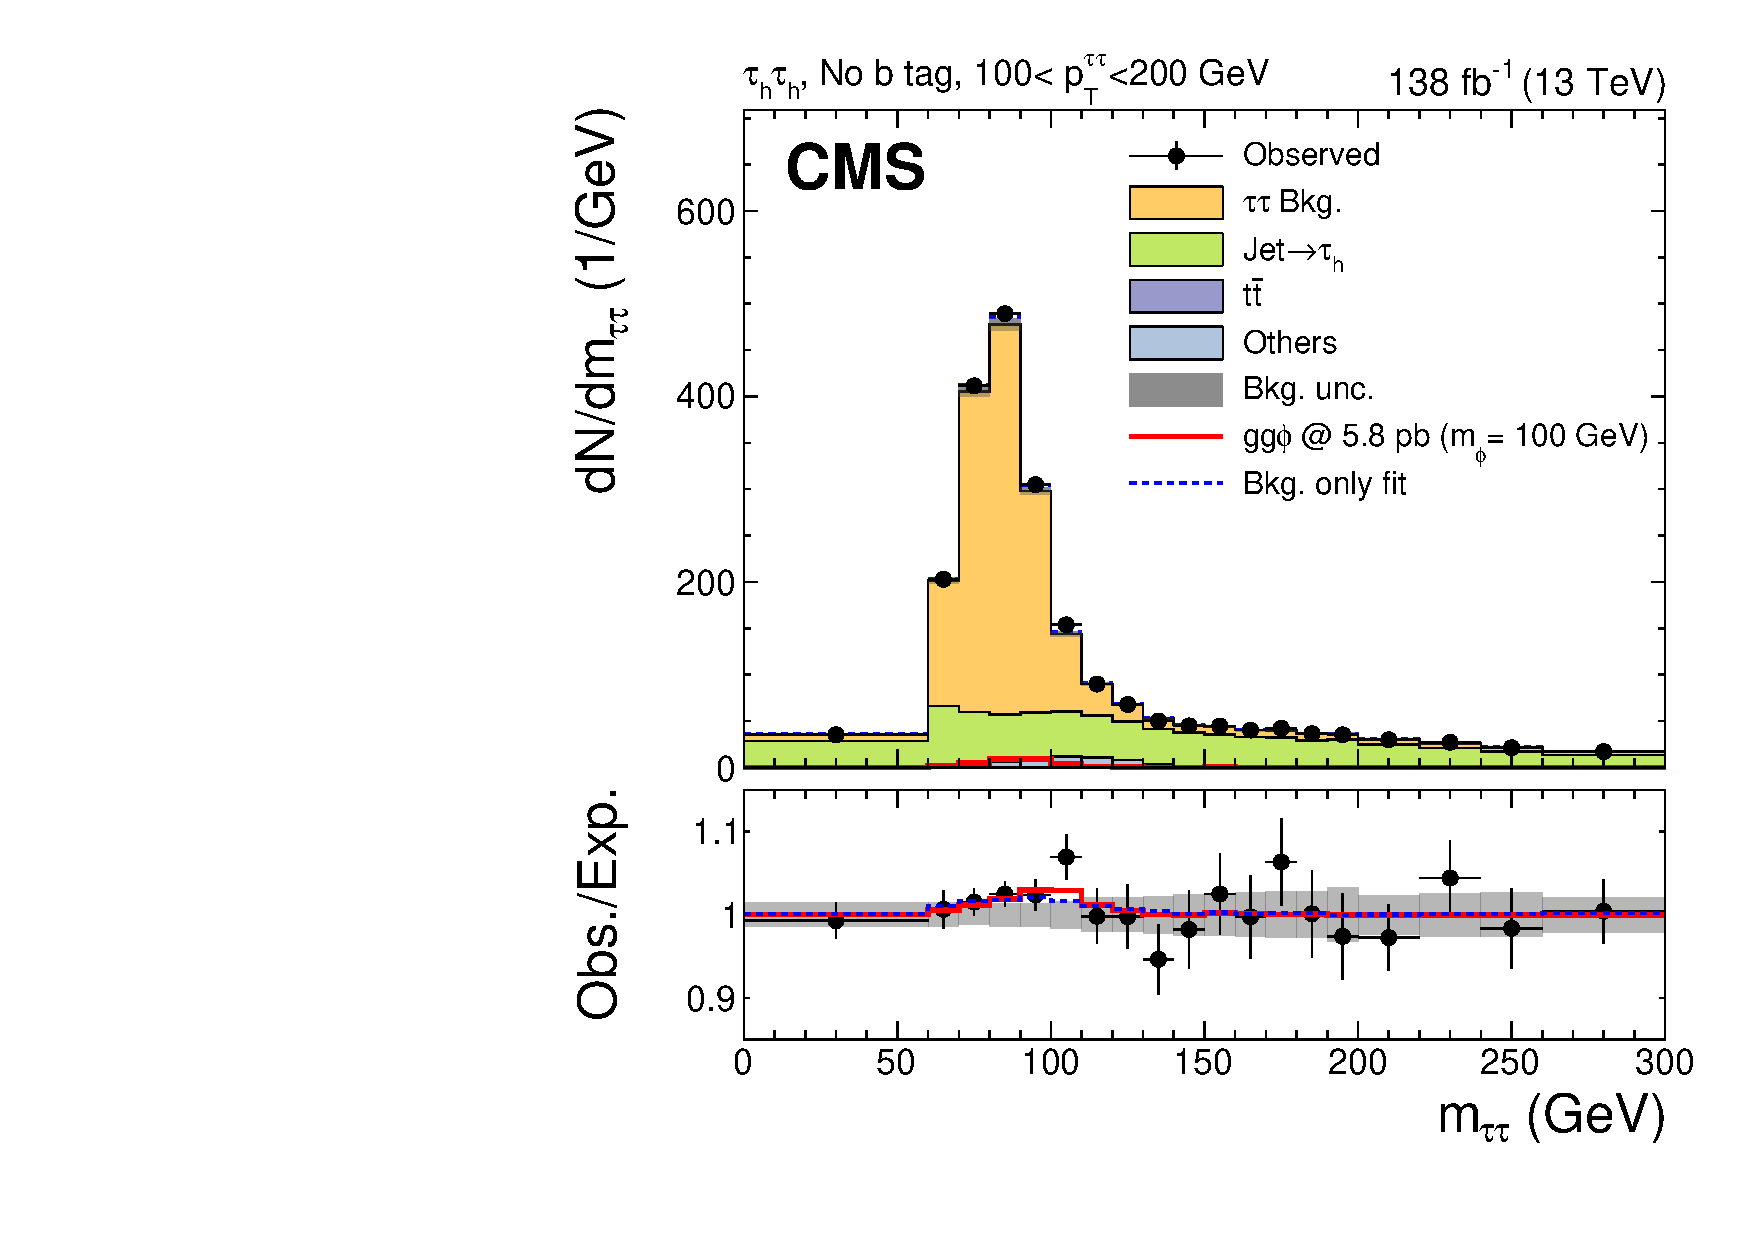
\includegraphics[width=0.4\textwidth]{Figures/postfit_lowmass_tt_nobtag_mediumpT.pdf}}
    \subfloat[]{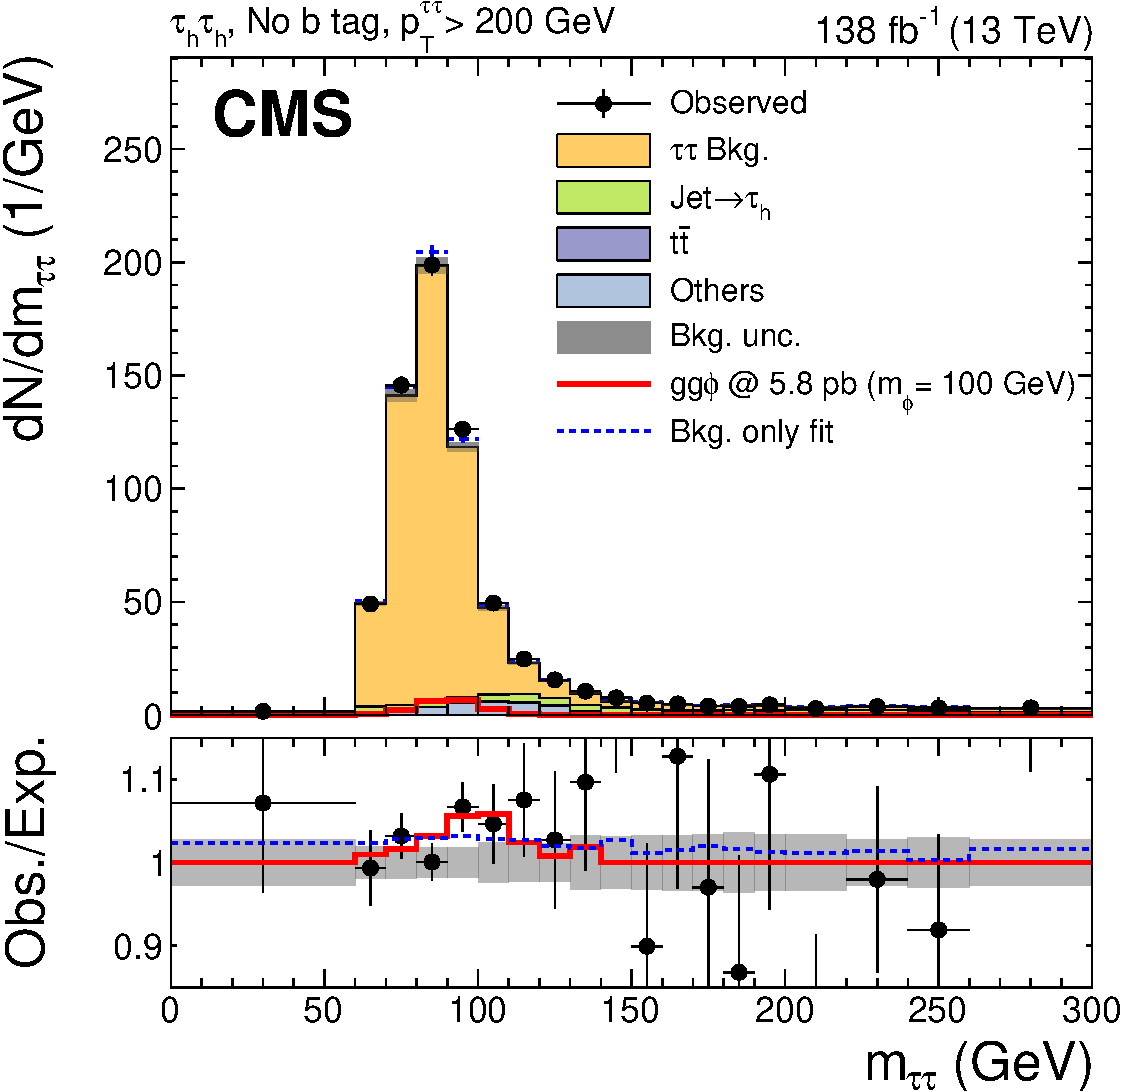
\includegraphics[width=0.4\textwidth]{Figures/postfit_lowmass_tt_nobtag_highpT-cropped.pdf}} \\
    \subfloat[]{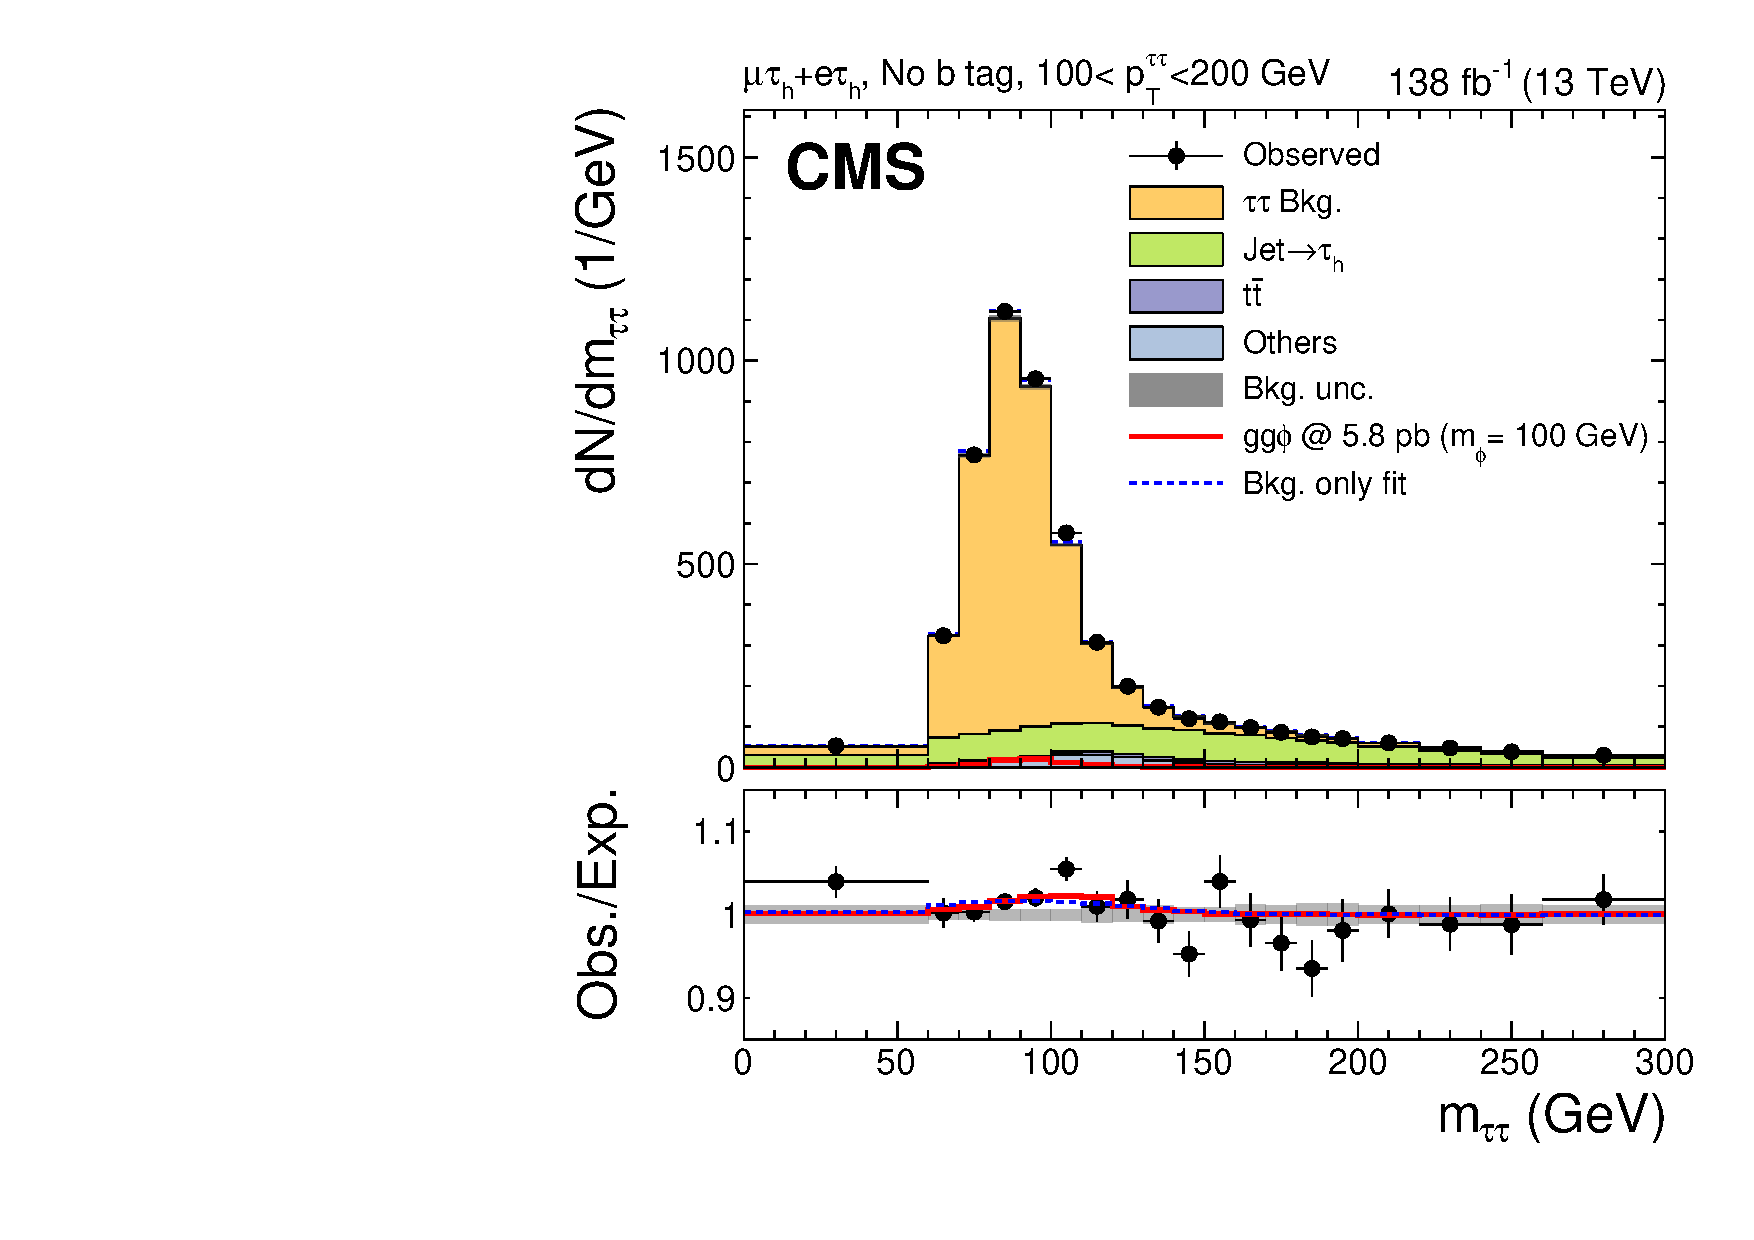
\includegraphics[width=0.4\textwidth]{Figures/postfit_lowmass_lt_nobtag_mediumpT.pdf}}
    \subfloat[]{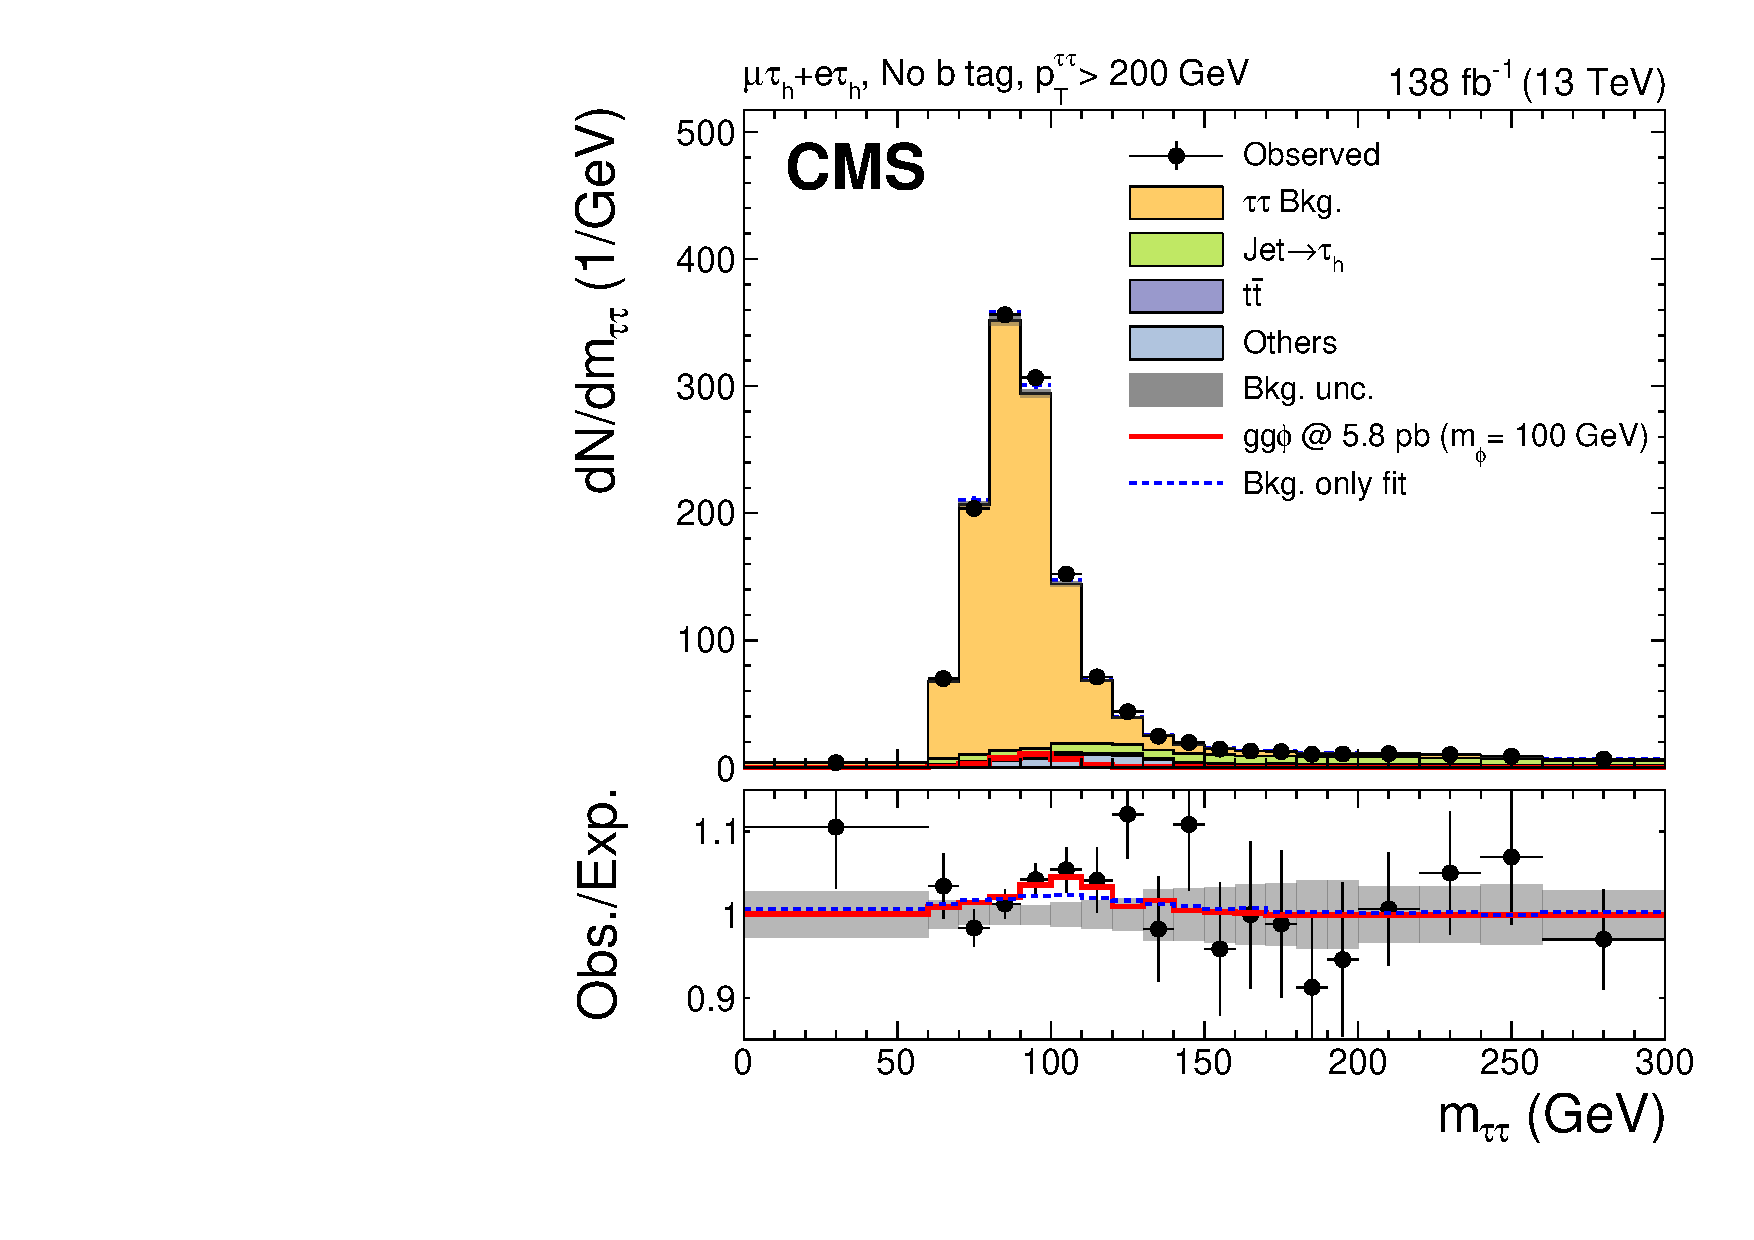
\includegraphics[width=0.4\textwidth]{Figures/postfit_lowmass_lt_nobtag_highpT.pdf}} \\
    \subfloat[]{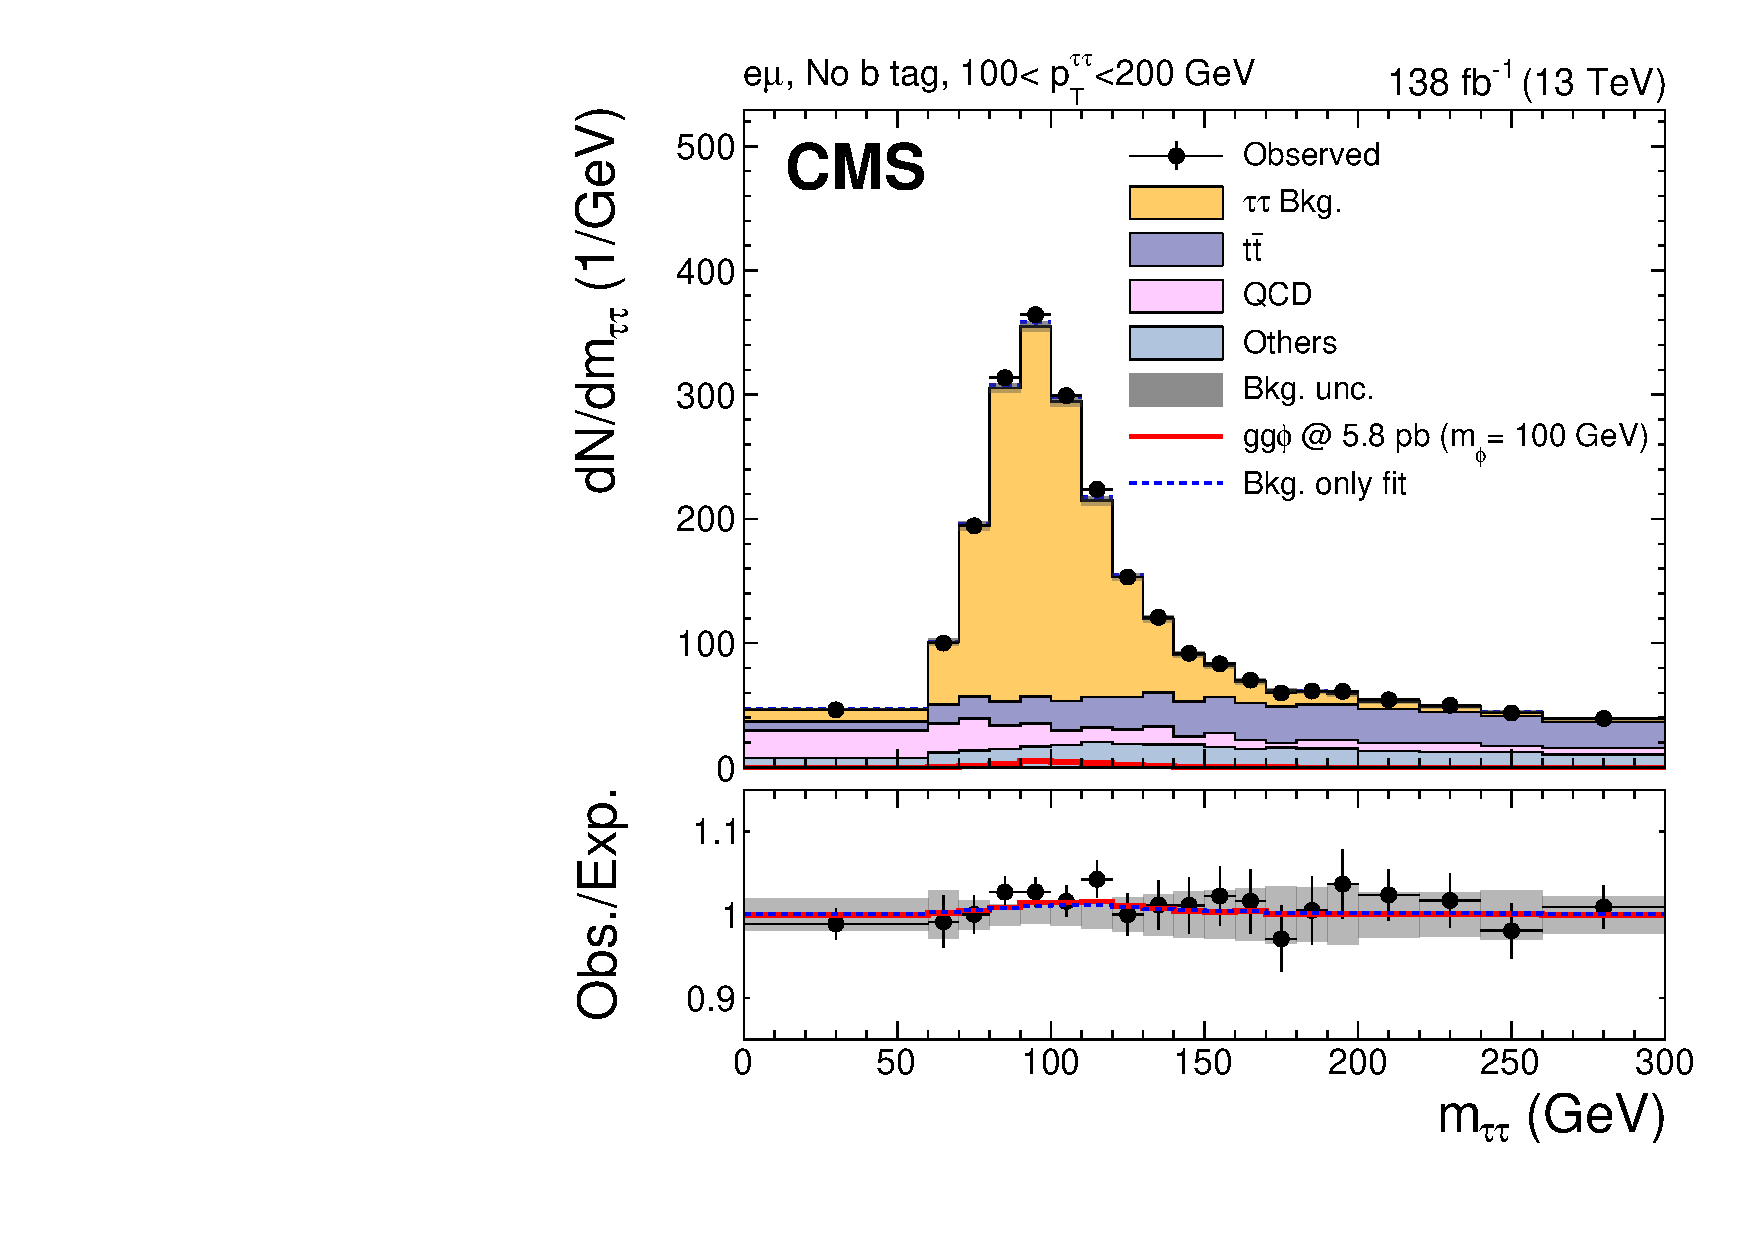
\includegraphics[width=0.4\textwidth]{Figures/postfit_lowmass_em_nobtag_mediumpT.pdf}}
    \subfloat[]{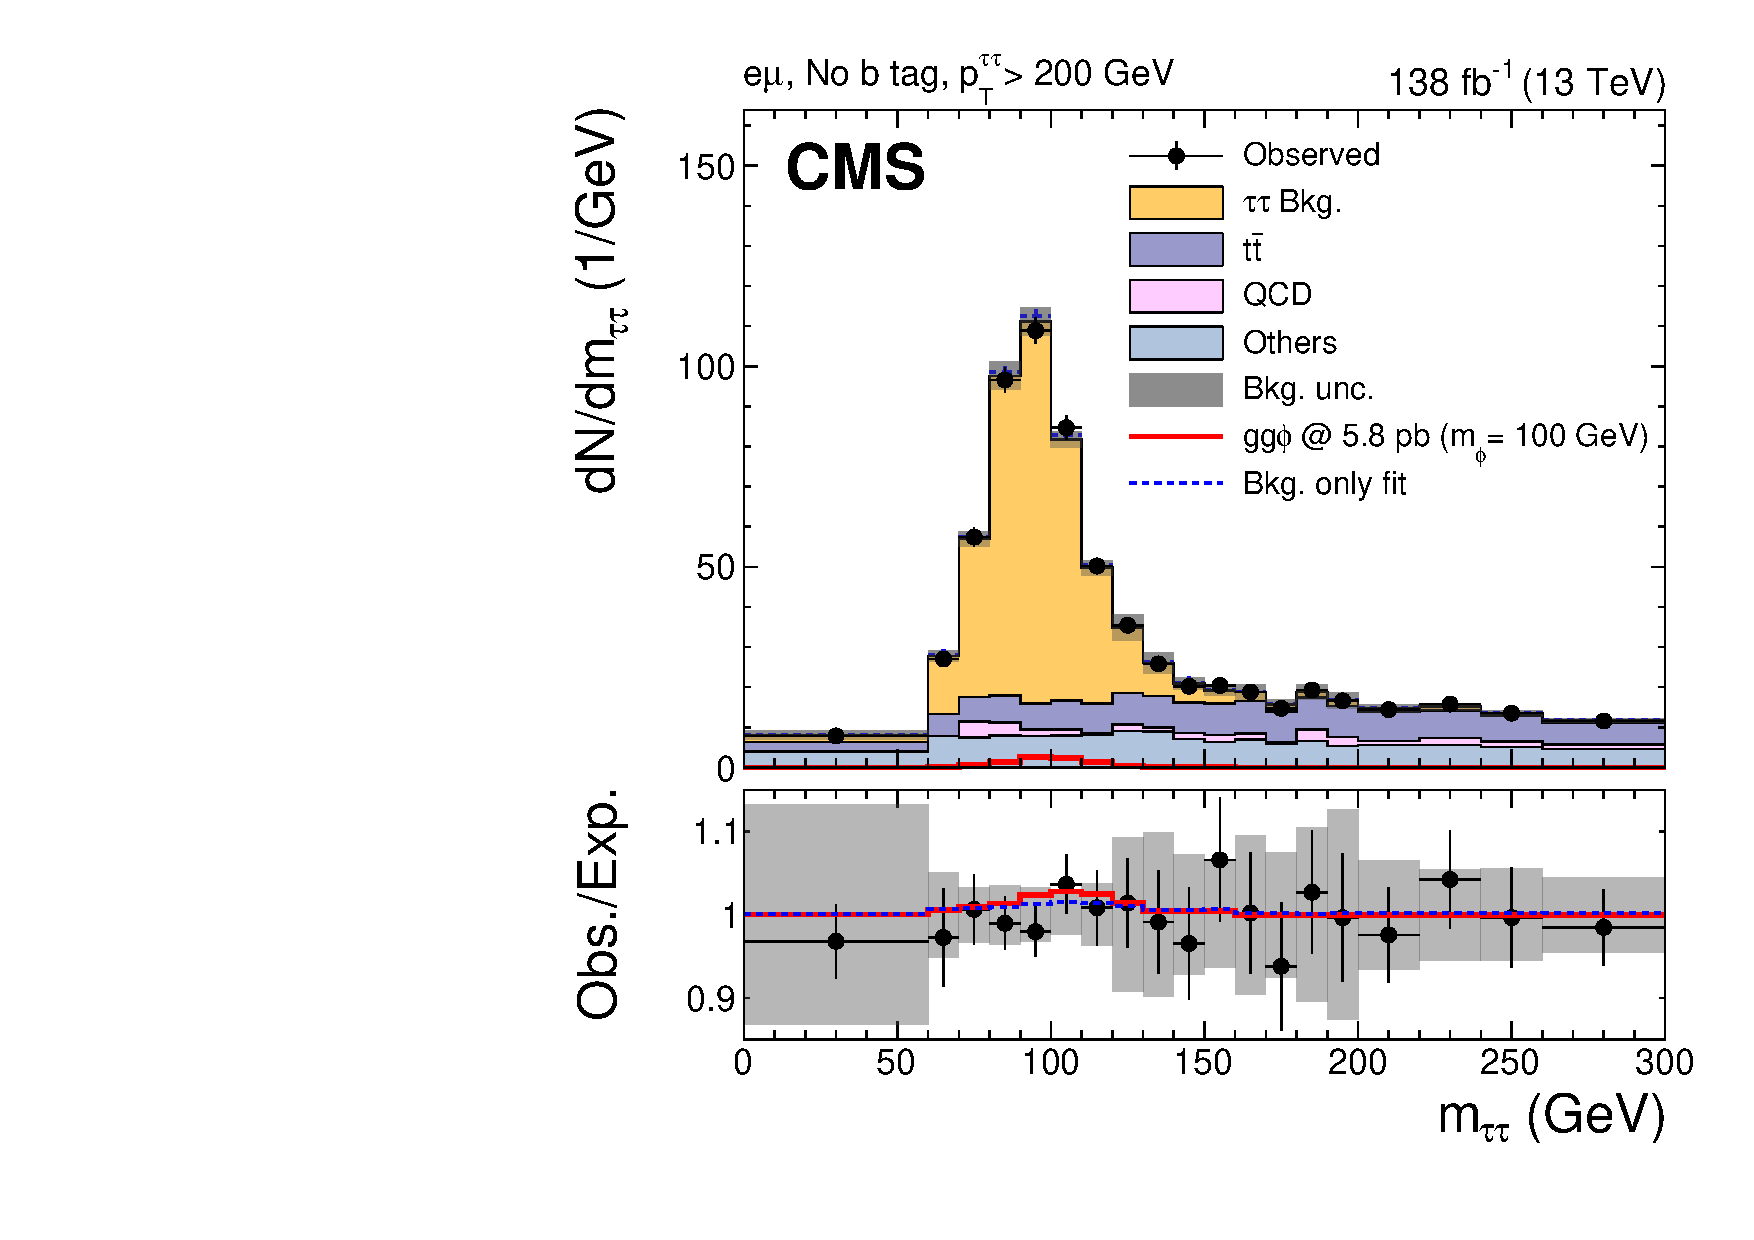
\includegraphics[width=0.4\textwidth]{Figures/postfit_lowmass_em_nobtag_highpT.pdf}}
\caption[Plots of the $m_{\tau\tau}$ distributions in the low-mass optimisation categories.]{Distributions of $m_{\tau\tau}$ in the no b tag second highest (a, c and e) and highest (b, d and e) $\pT$ category for the $\tauhtauh$ (a and b), the combined $\etauh$ and $\mutauh$ (c and d) and the $\emu$ (d and e) channels. The solid histograms show the stacked background predictions after a signal-plus-background fit to the data. The best-fit gluon fusion signal for $m_{\phi}$ = 100 GeV is shown by the red line. Also shown by a blue dashed line on the bottom pad is the ratio of the background predictions for the background-only fit to the signal-plus-background fit~\cite{CMS:2022rbd}. }
\label{fig:low_mass_postfit}
\end{figure}

\begin{figure}[!hbtp]
\centering
    \subfloat[]{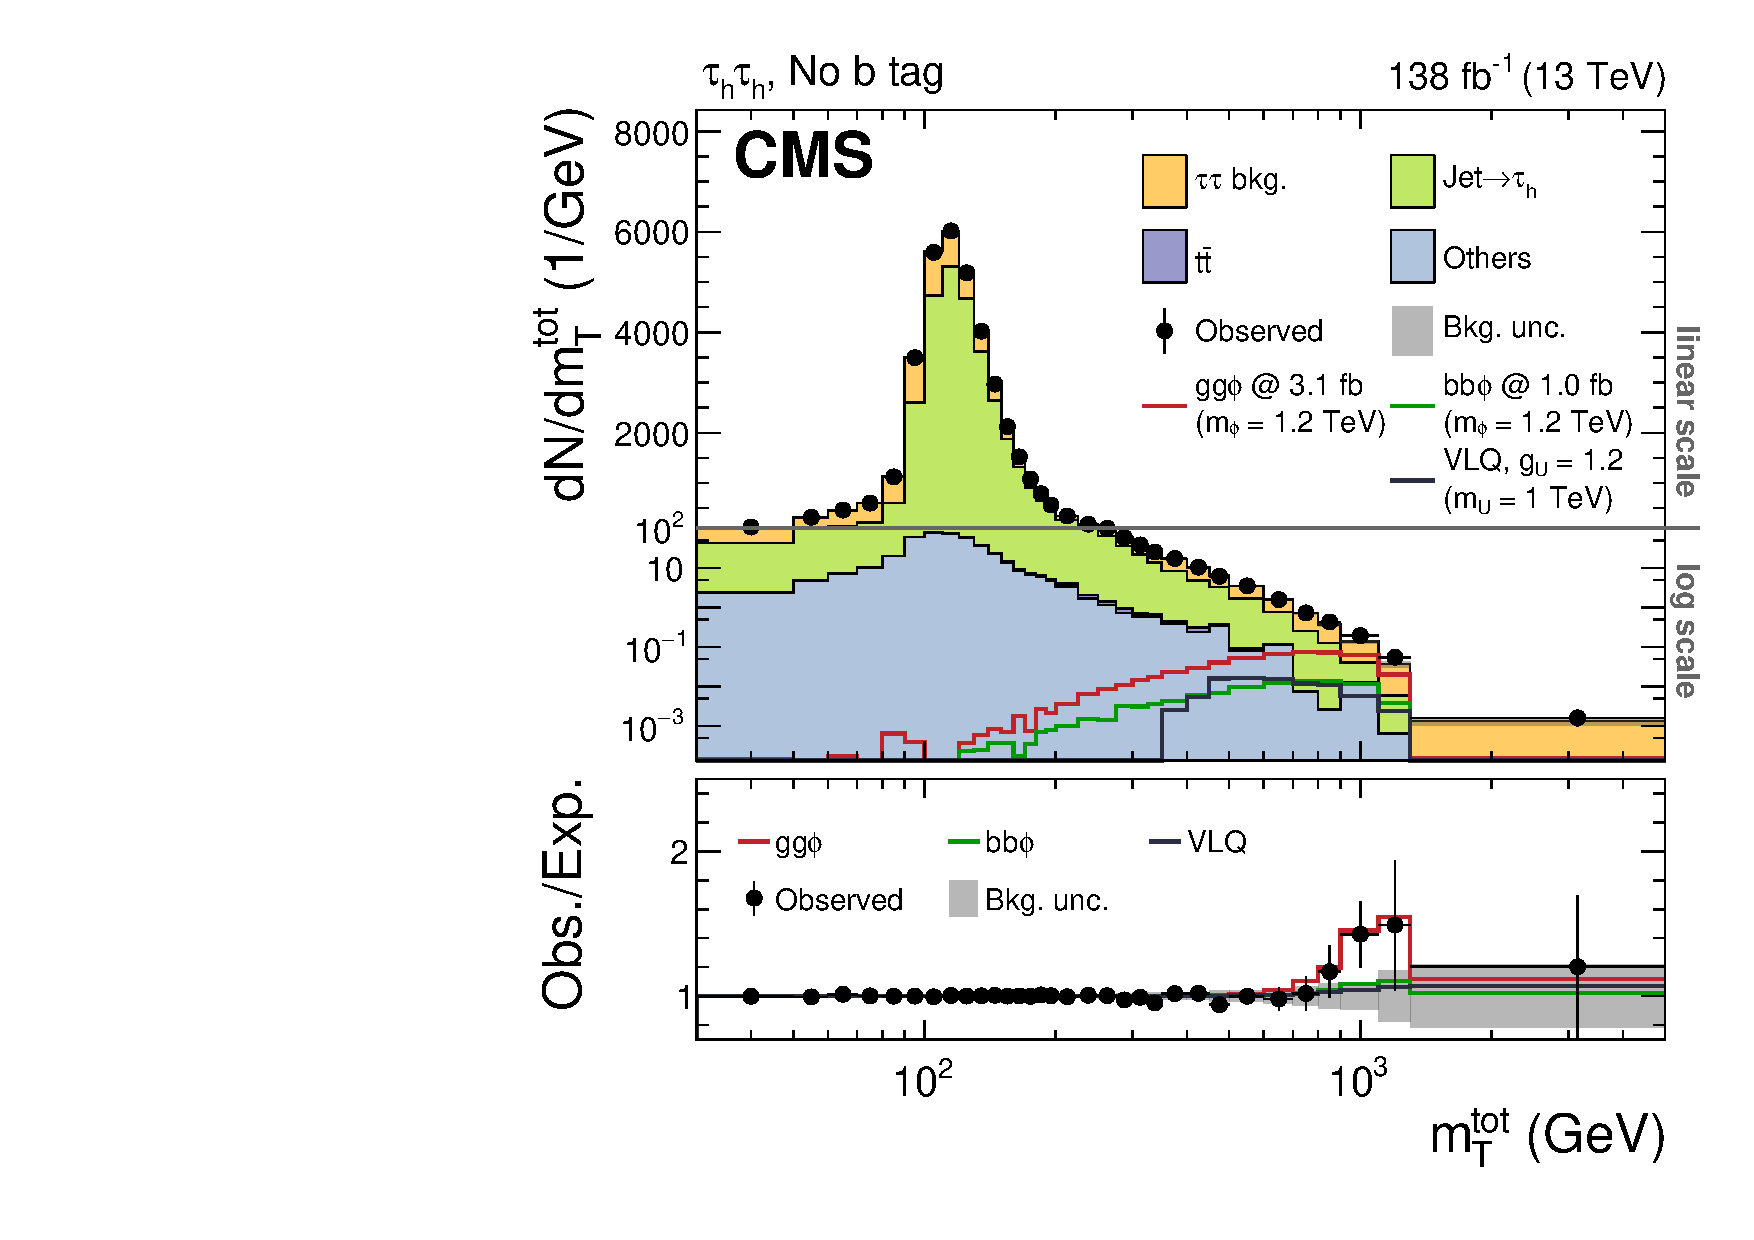
\includegraphics[width=0.42\textwidth]{Figures/postfit_highmass_tt_nobtag.pdf}}
    \subfloat[]{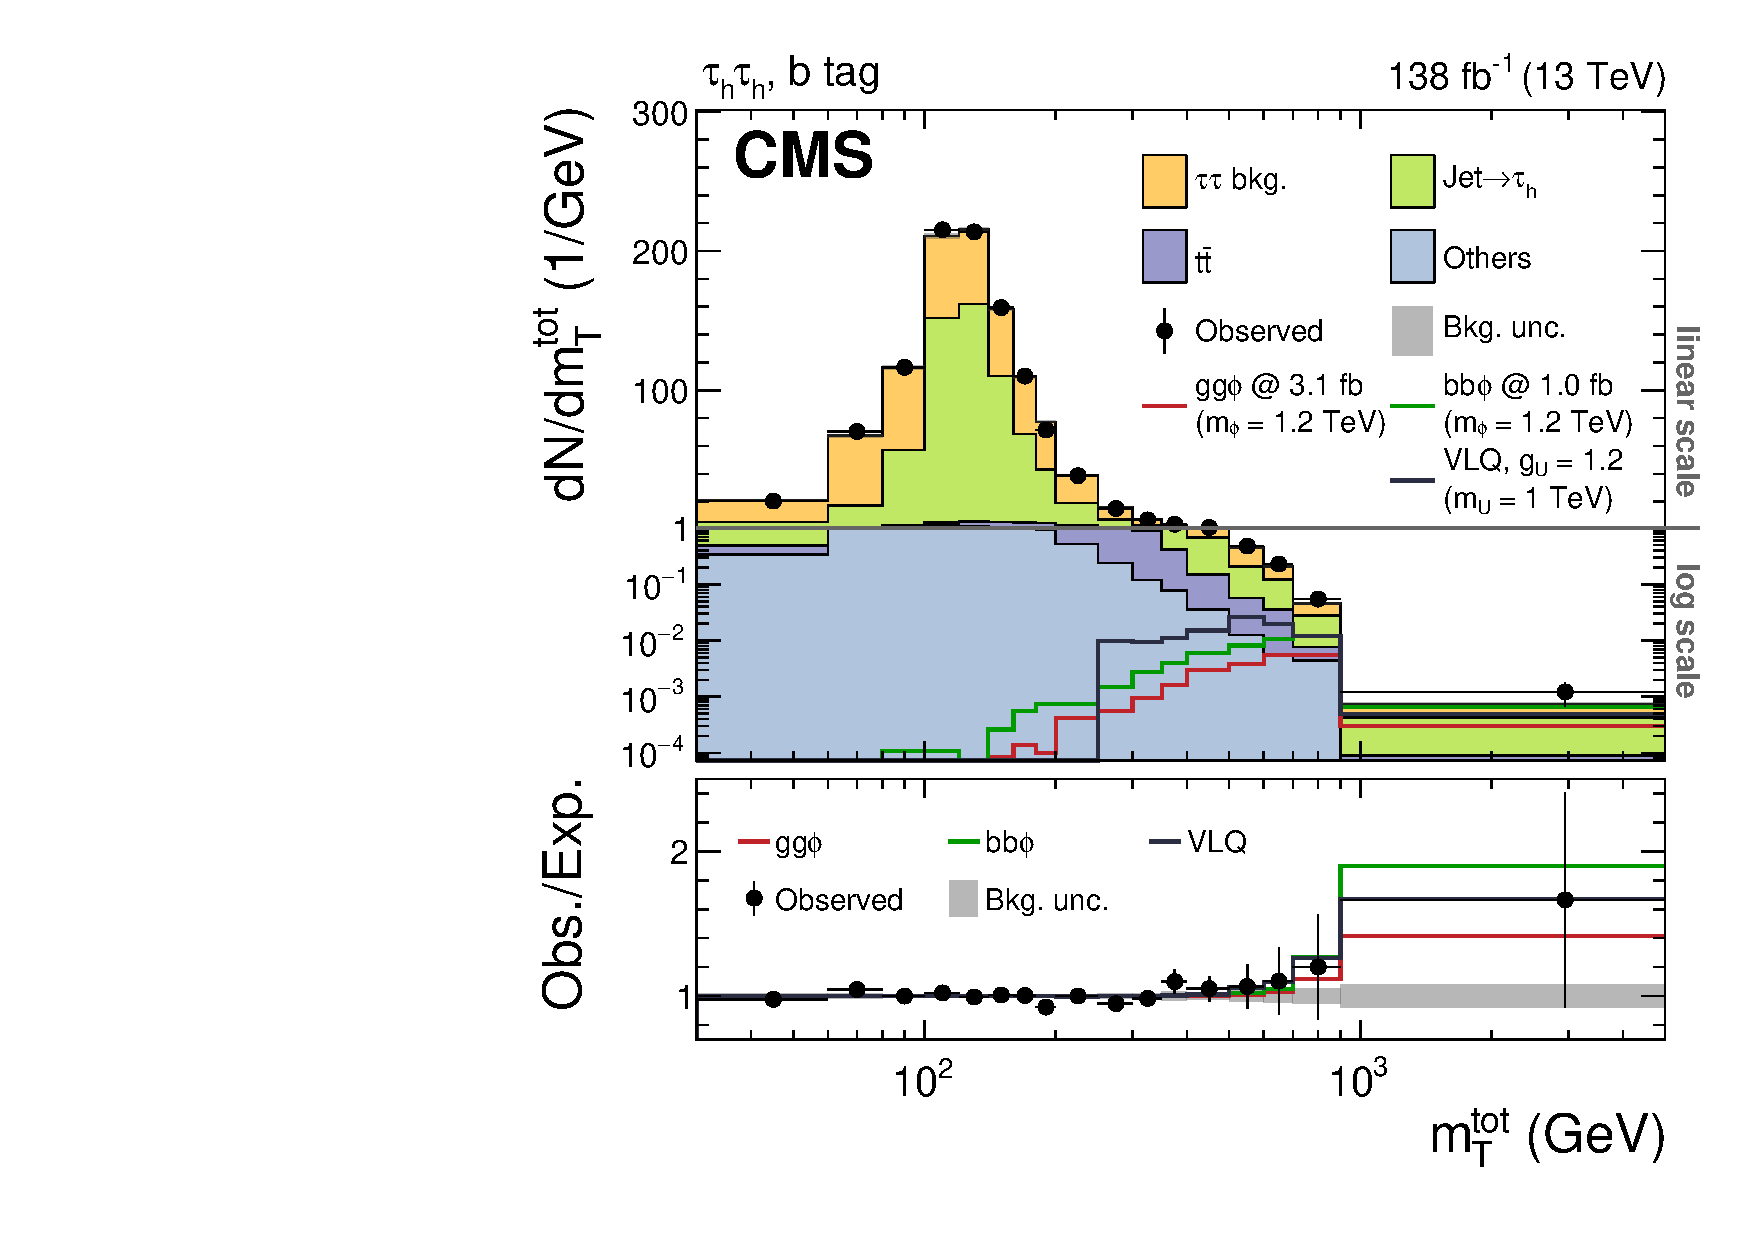
\includegraphics[width=0.42\textwidth]{Figures/postfit_highmass_tt_btag.pdf}} \\
    \subfloat[]{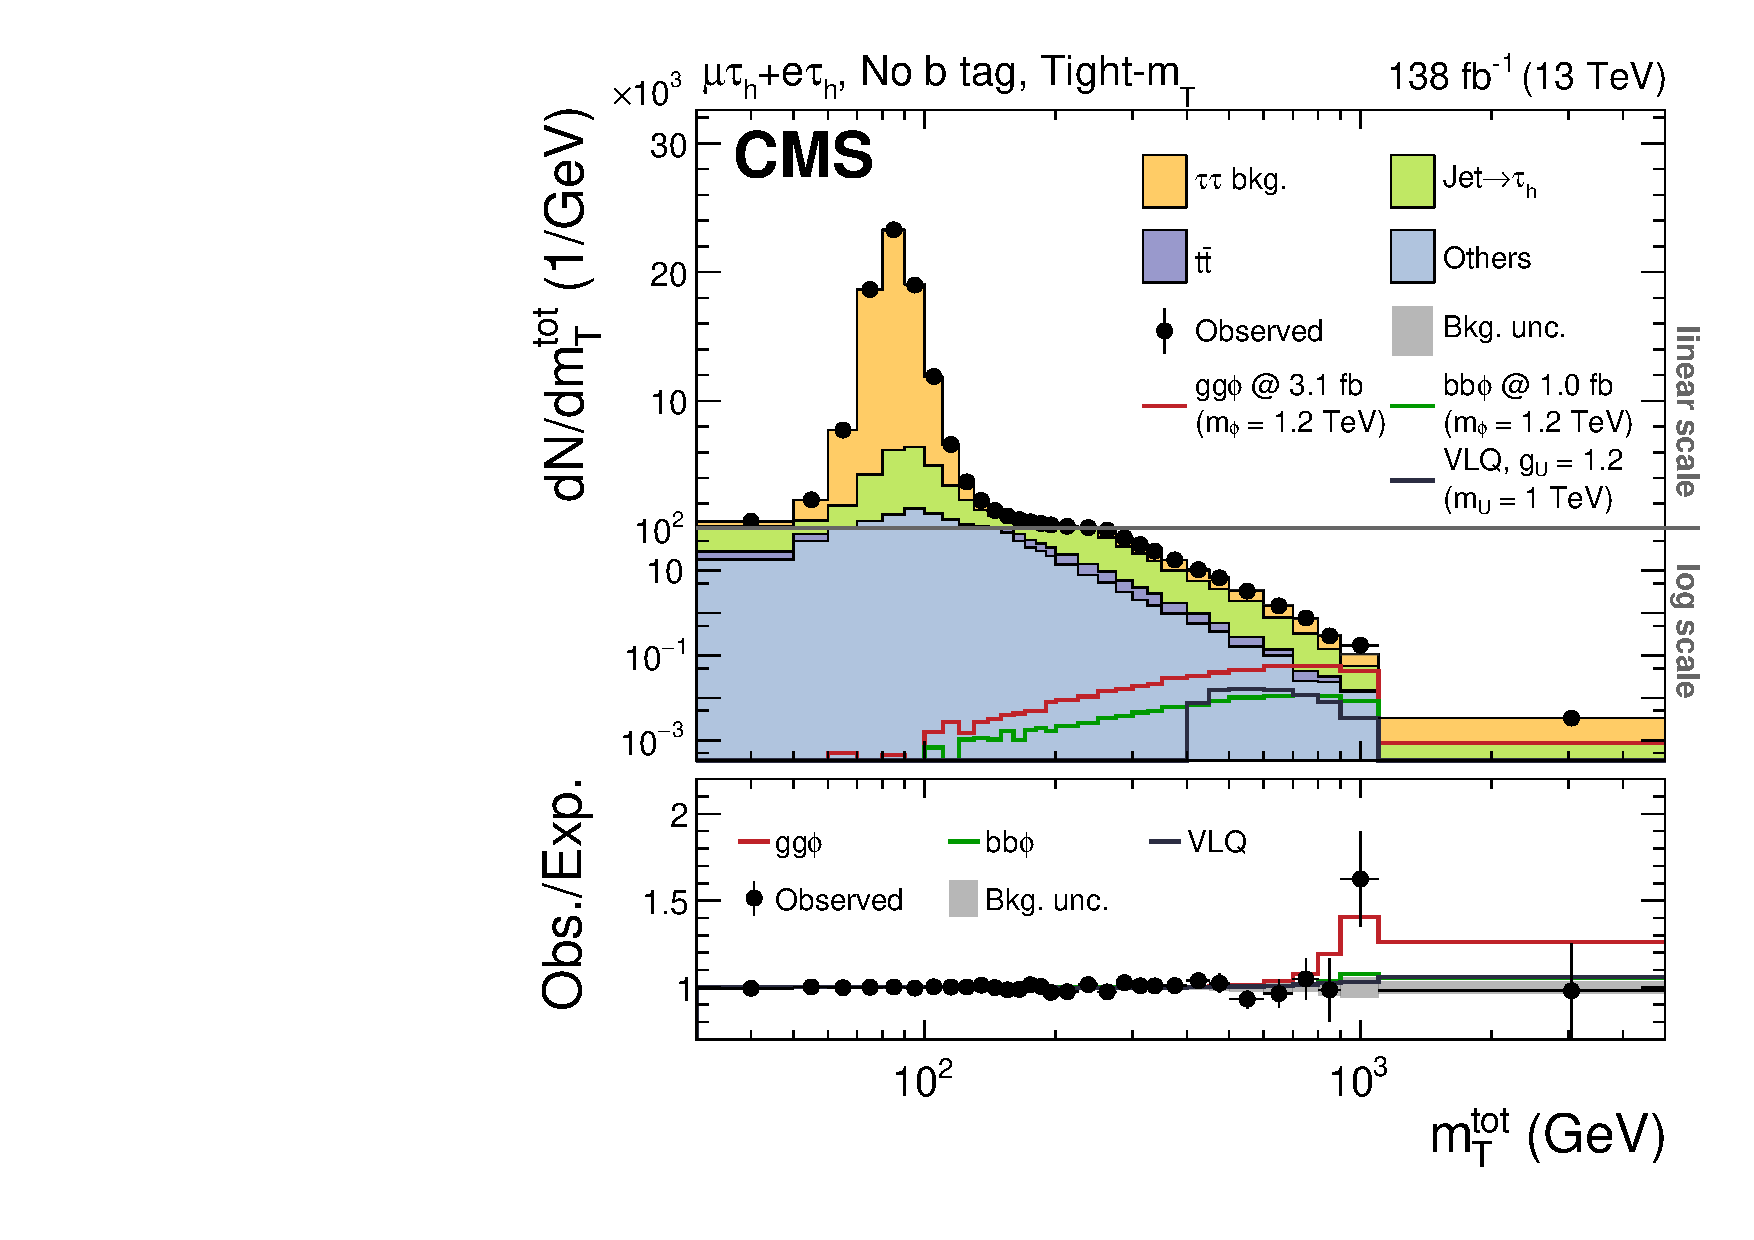
\includegraphics[width=0.42\textwidth]{Figures/postfit_highmass_lt_nobtag_tightmT.pdf}}
    \subfloat[]{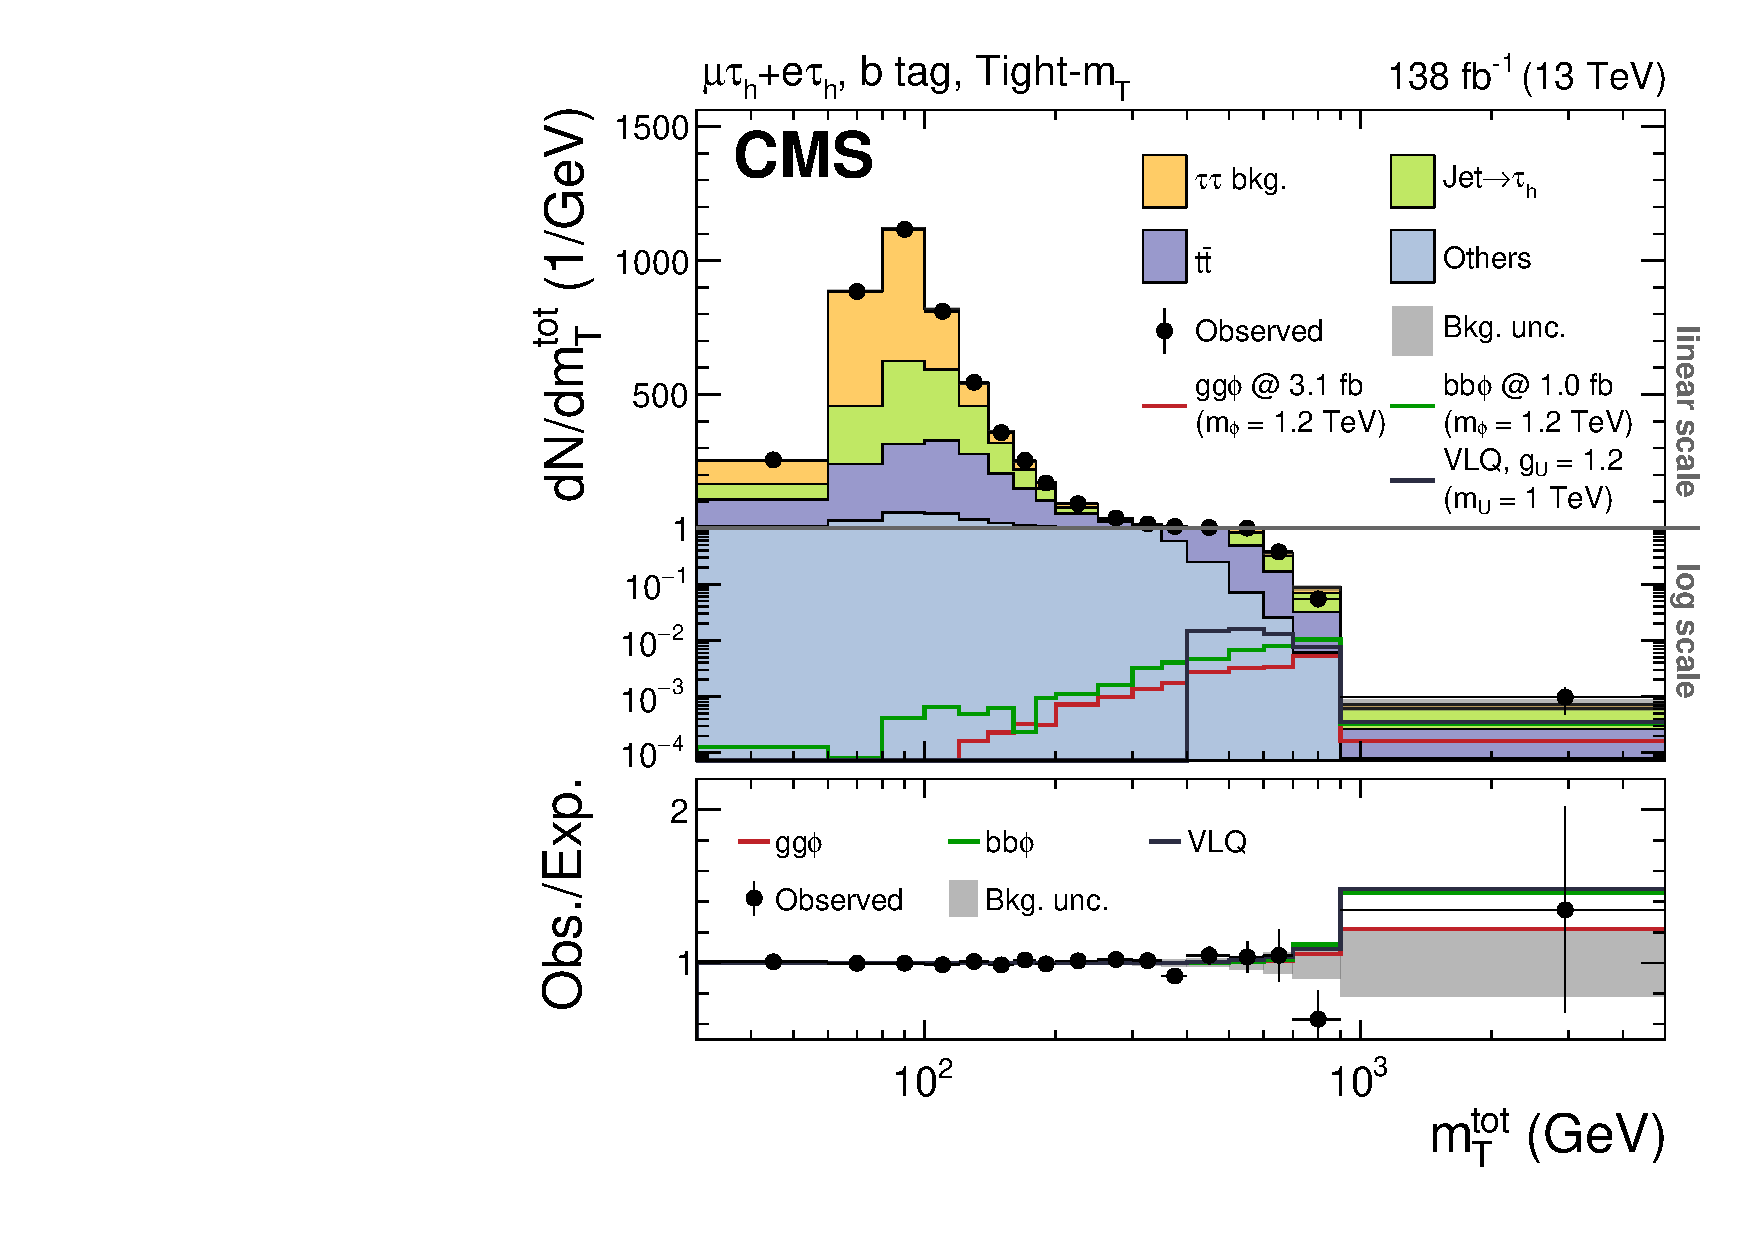
\includegraphics[width=0.42\textwidth]{Figures/postfit_highmass_lt_btag_tightmT.pdf}} \\
    \subfloat[]{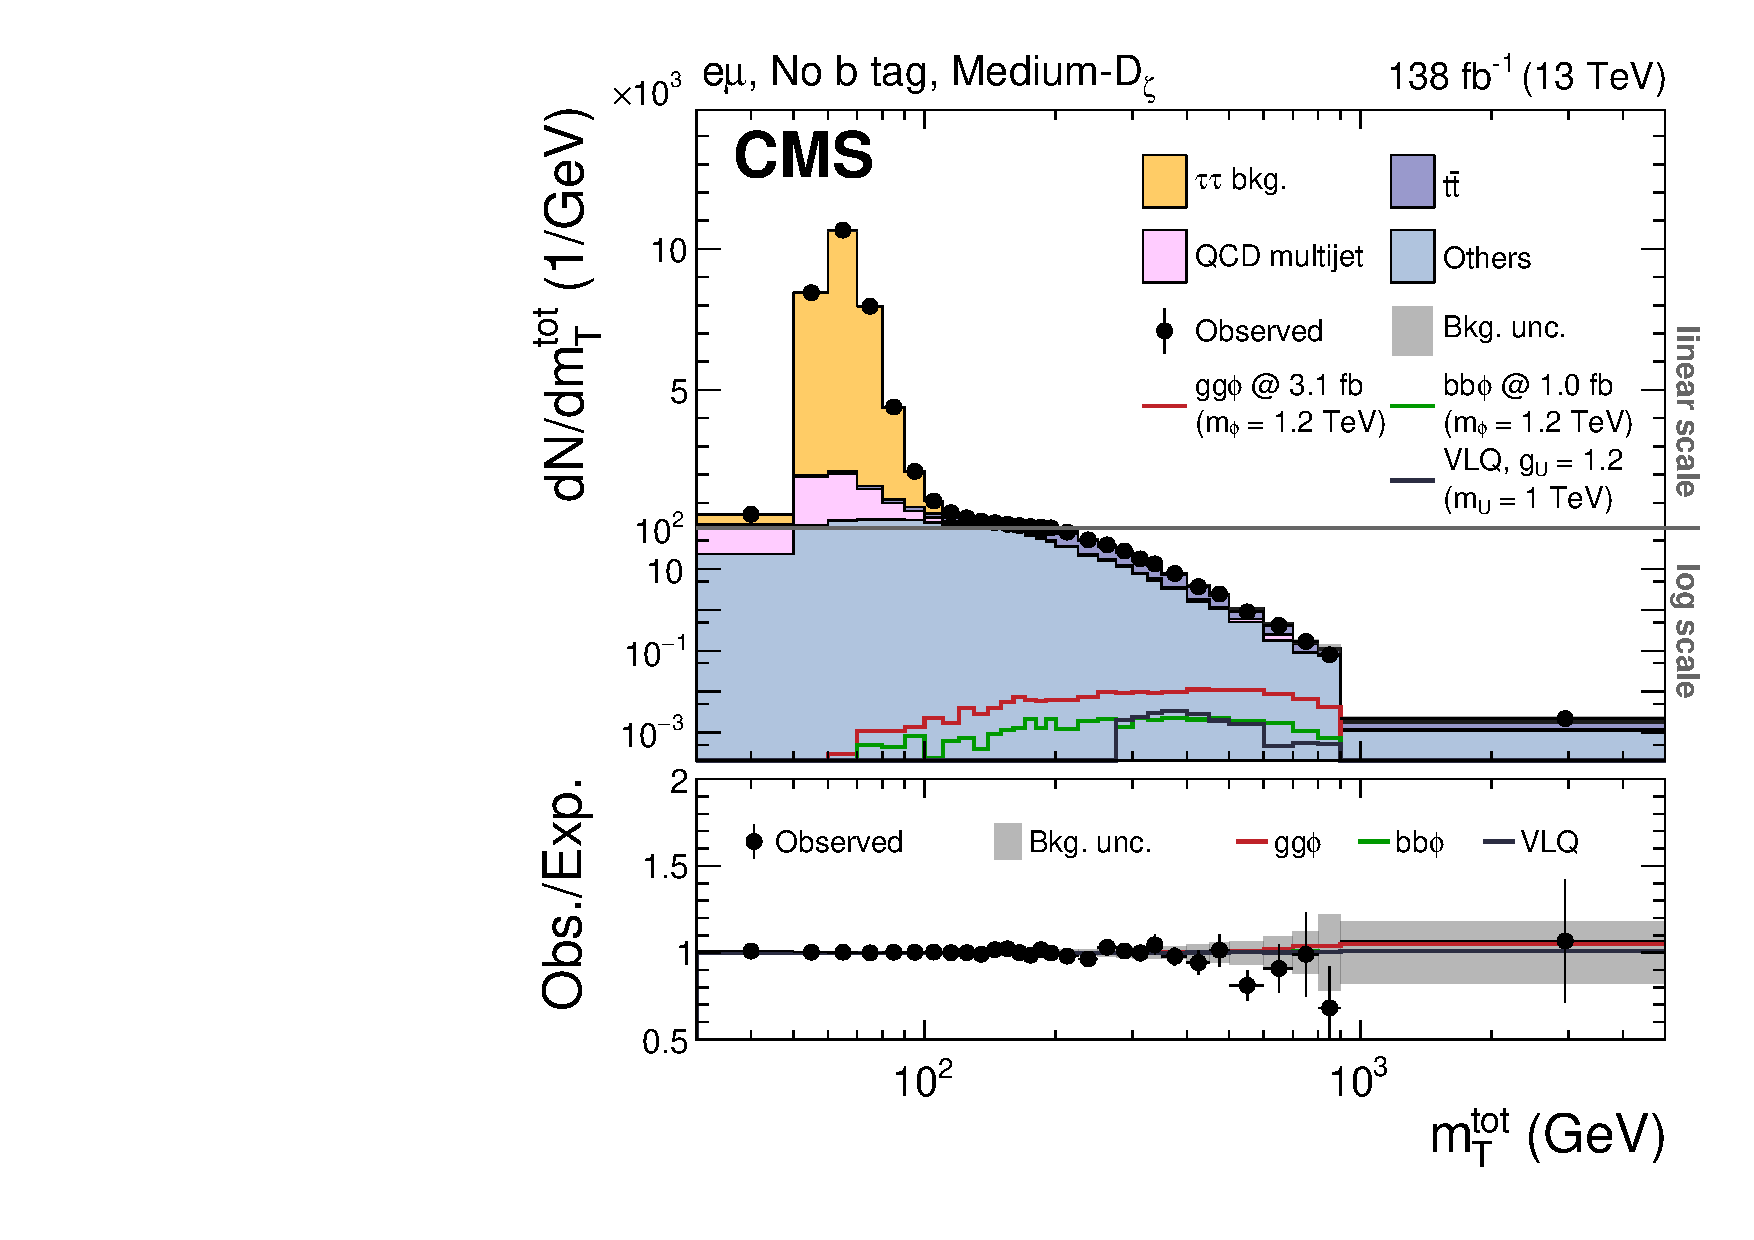
\includegraphics[width=0.42\textwidth]{Figures/postfit_highmass_em_nobtag_mediumdzeta.pdf}}
    \subfloat[]{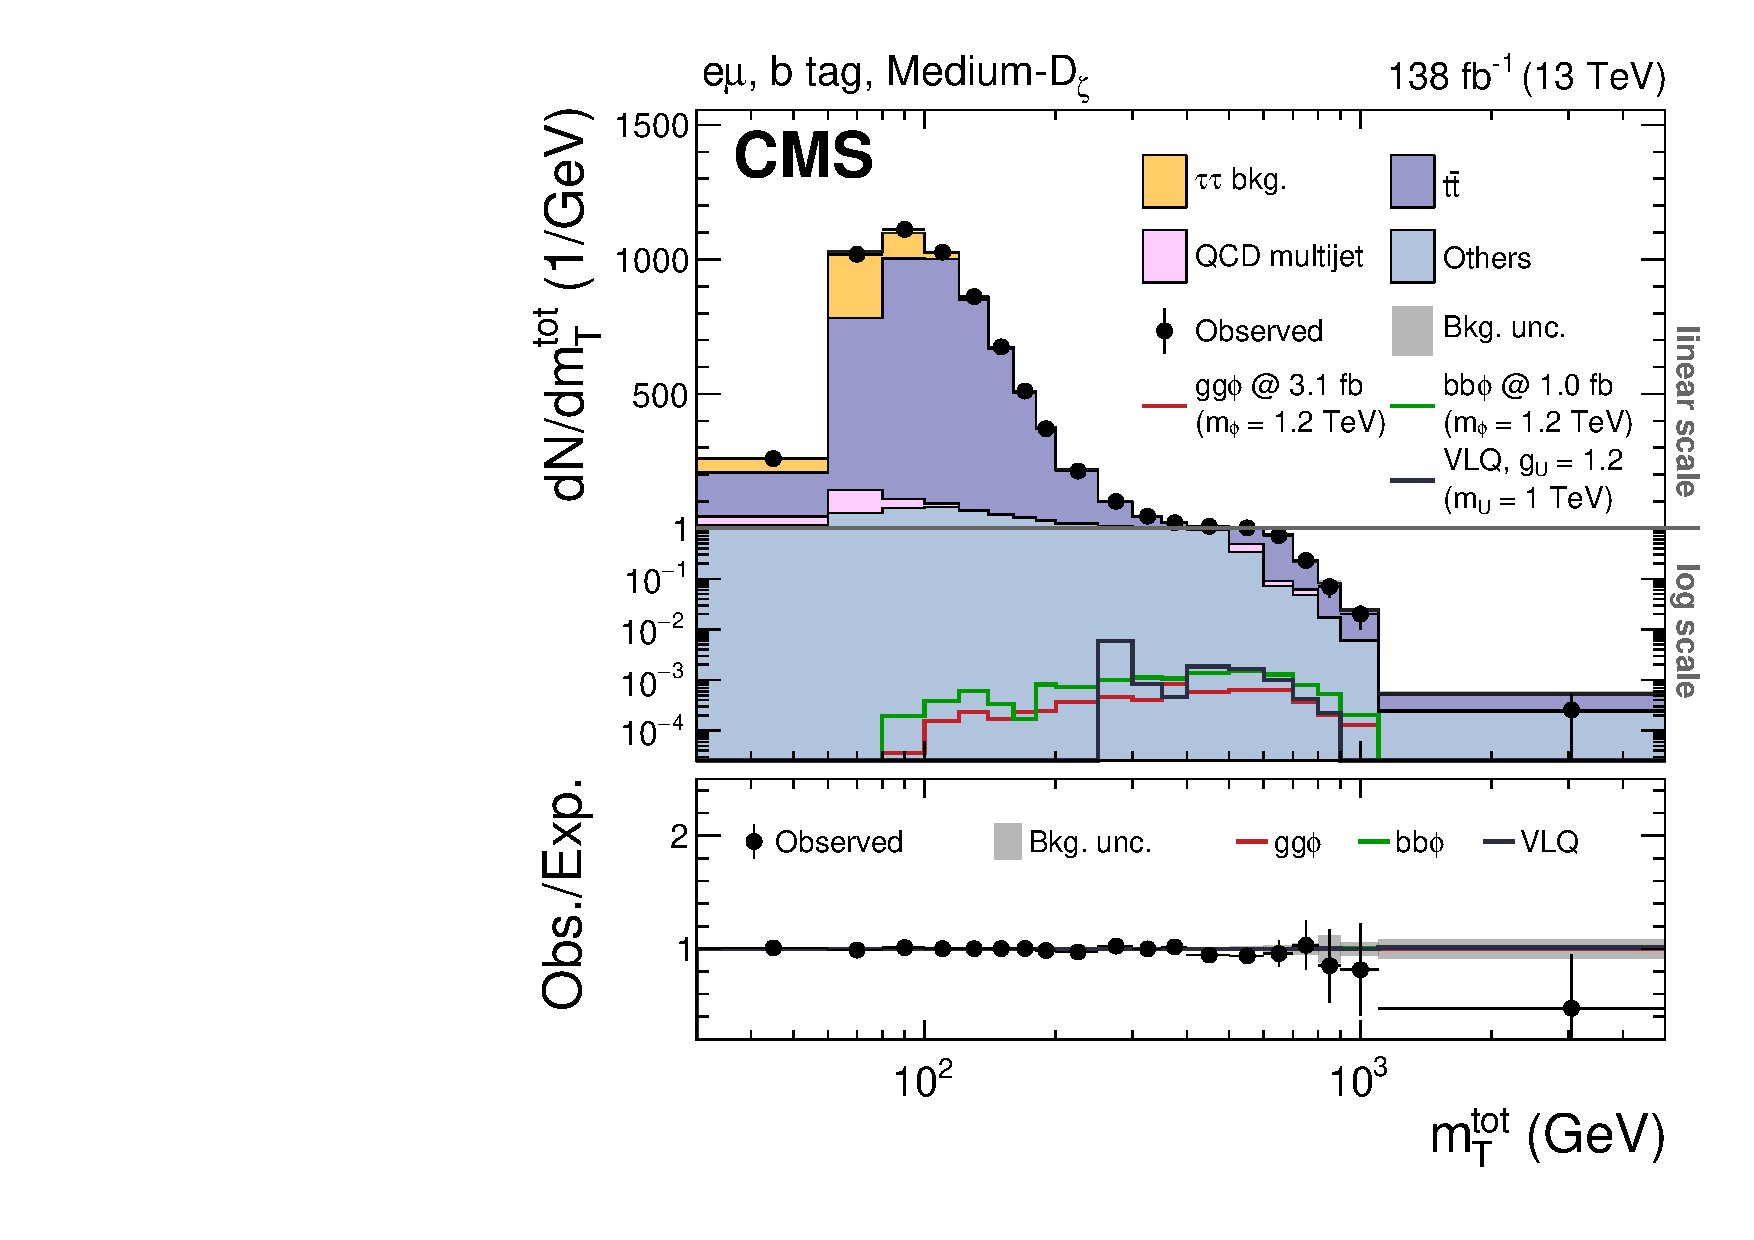
\includegraphics[width=0.42\textwidth]{Figures/postfit_highmass_em_btag_mediumdzeta.pdf}}
\caption[Plots of the $m_{T}^\text{tot}$ distributions in the high-mass optimisation categories.]{Distributions of $m_{T}^\text{tot}$ in the $\tauhtauh$ no b tag (a) and b tag (b) categories, the combined $\etauh$ and $\mutauh$ no b tag (c) and b tag (d) \texttt{Tight-$m_{T}$} categories and the $\emu$ no b tag (e) and b tag (f) \texttt{Medium-$D_{\zeta}$} categories. The solid histograms show the stacked background predictions after a background-only fit to the data. The best-fit gluon fusion signal for $m_{\phi}$ = 1.2 TeV is shown by the red line, b-associated production and $U_{1}$ signals are also shown for illustrative purposes~\cite{CMS:2022rbd}.}
\label{fig:high_mass_postfit}
\end{figure}

\section{Model-independent results}

\subsection{Limits}

95\% \ac{CL} limits are set on the assumption of the absence of a signal for the search for a gg$\phi$ or bb$\phi$ resonance and these are shown in Figure~\ref{fig:model_independent_limits}.
In each case, the other process is allowed to float freely in the fit.
The excesses observed in the postfit distributions act to weaken the observed limit compared to the expected limit at 100 GeV and 1.2 TeV, as more data was observed than expected.
For gg$\phi$ production, the expected limits flatten under 100 GeV, due to the difficulty of separating the signal from the Z boson at this mass.
Both sets of limits vary from $\mathcal{O}(10\text{ pb})$ at 60 GeV to $0.3$ fb at 3.5 TeV. \\

\begin{figure}[!hbtp]
\centering
    \subfloat[]{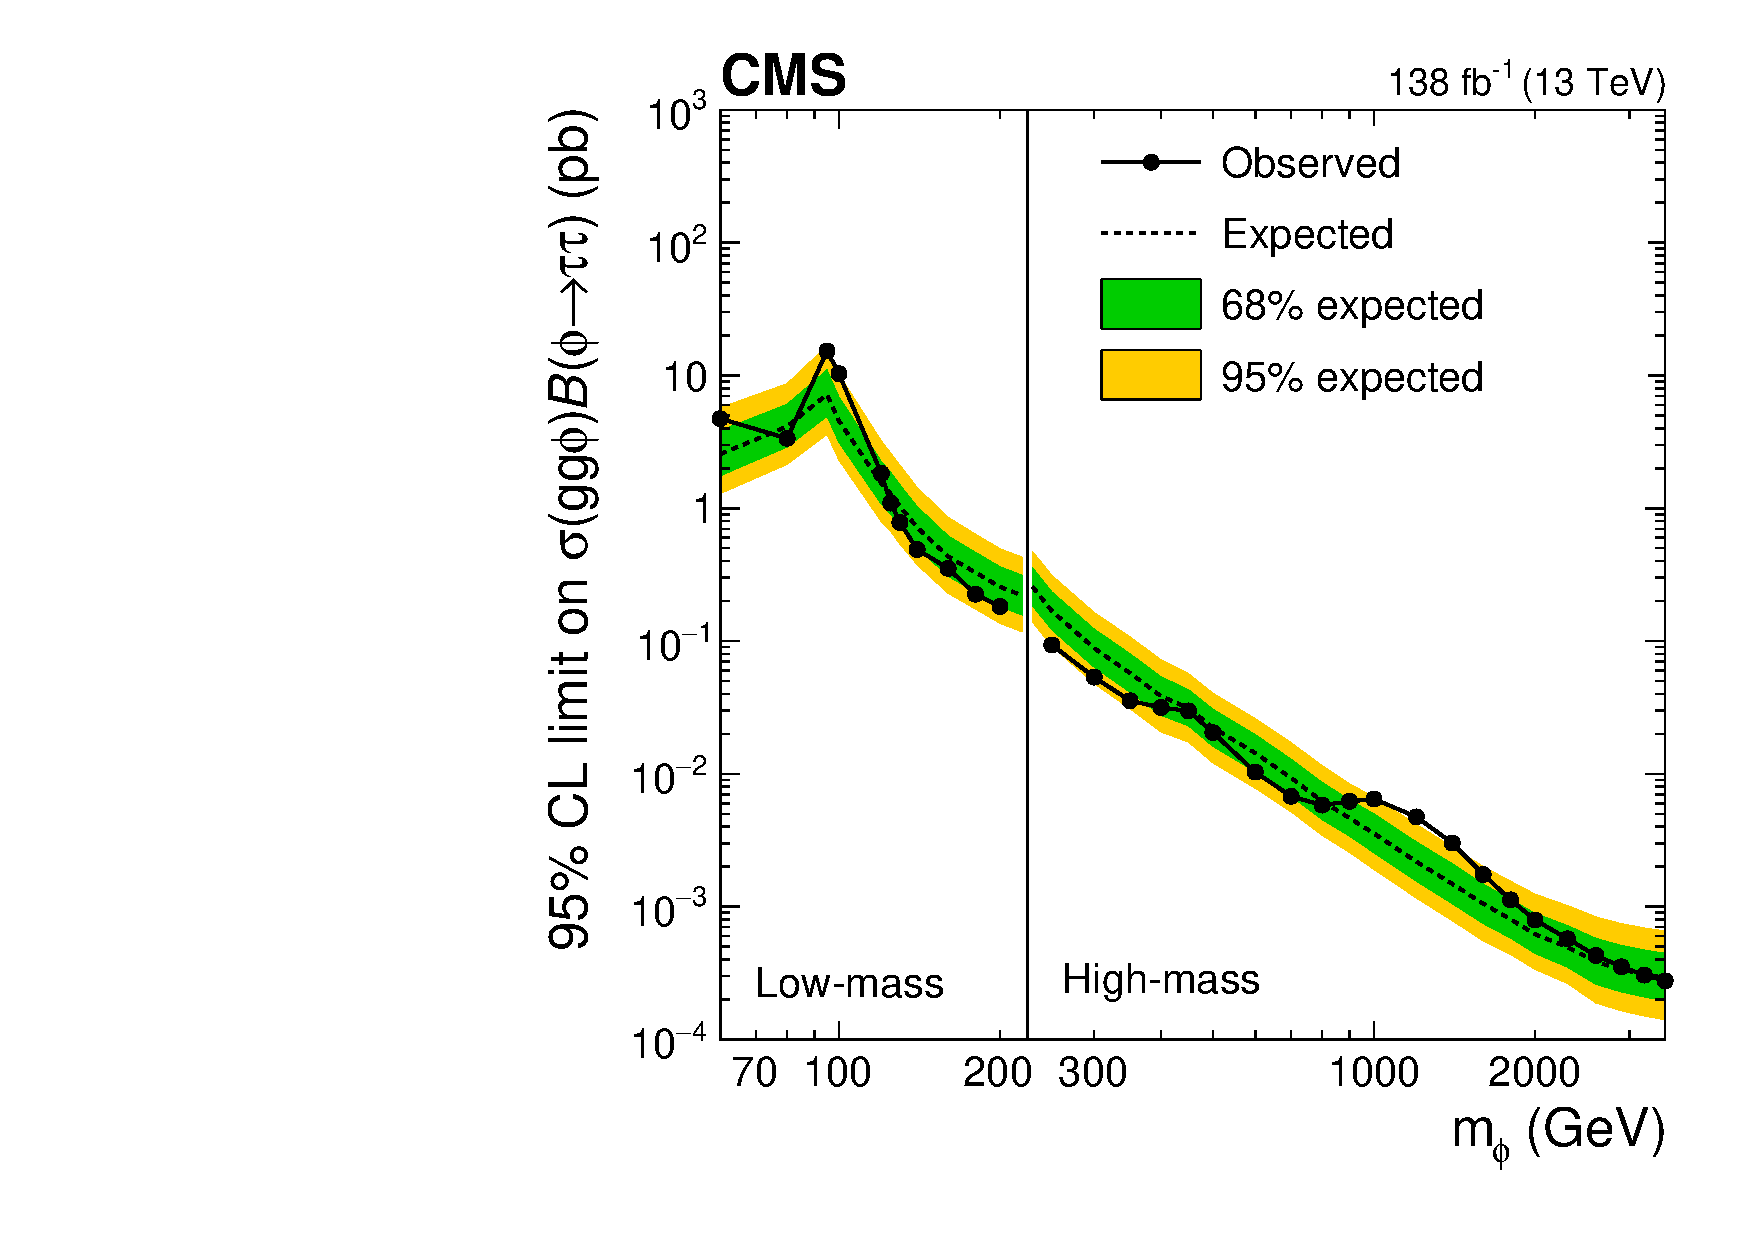
\includegraphics[width=0.65\textwidth]{Figures/model_independent_limit_ggH.pdf}} \\
    \subfloat[]{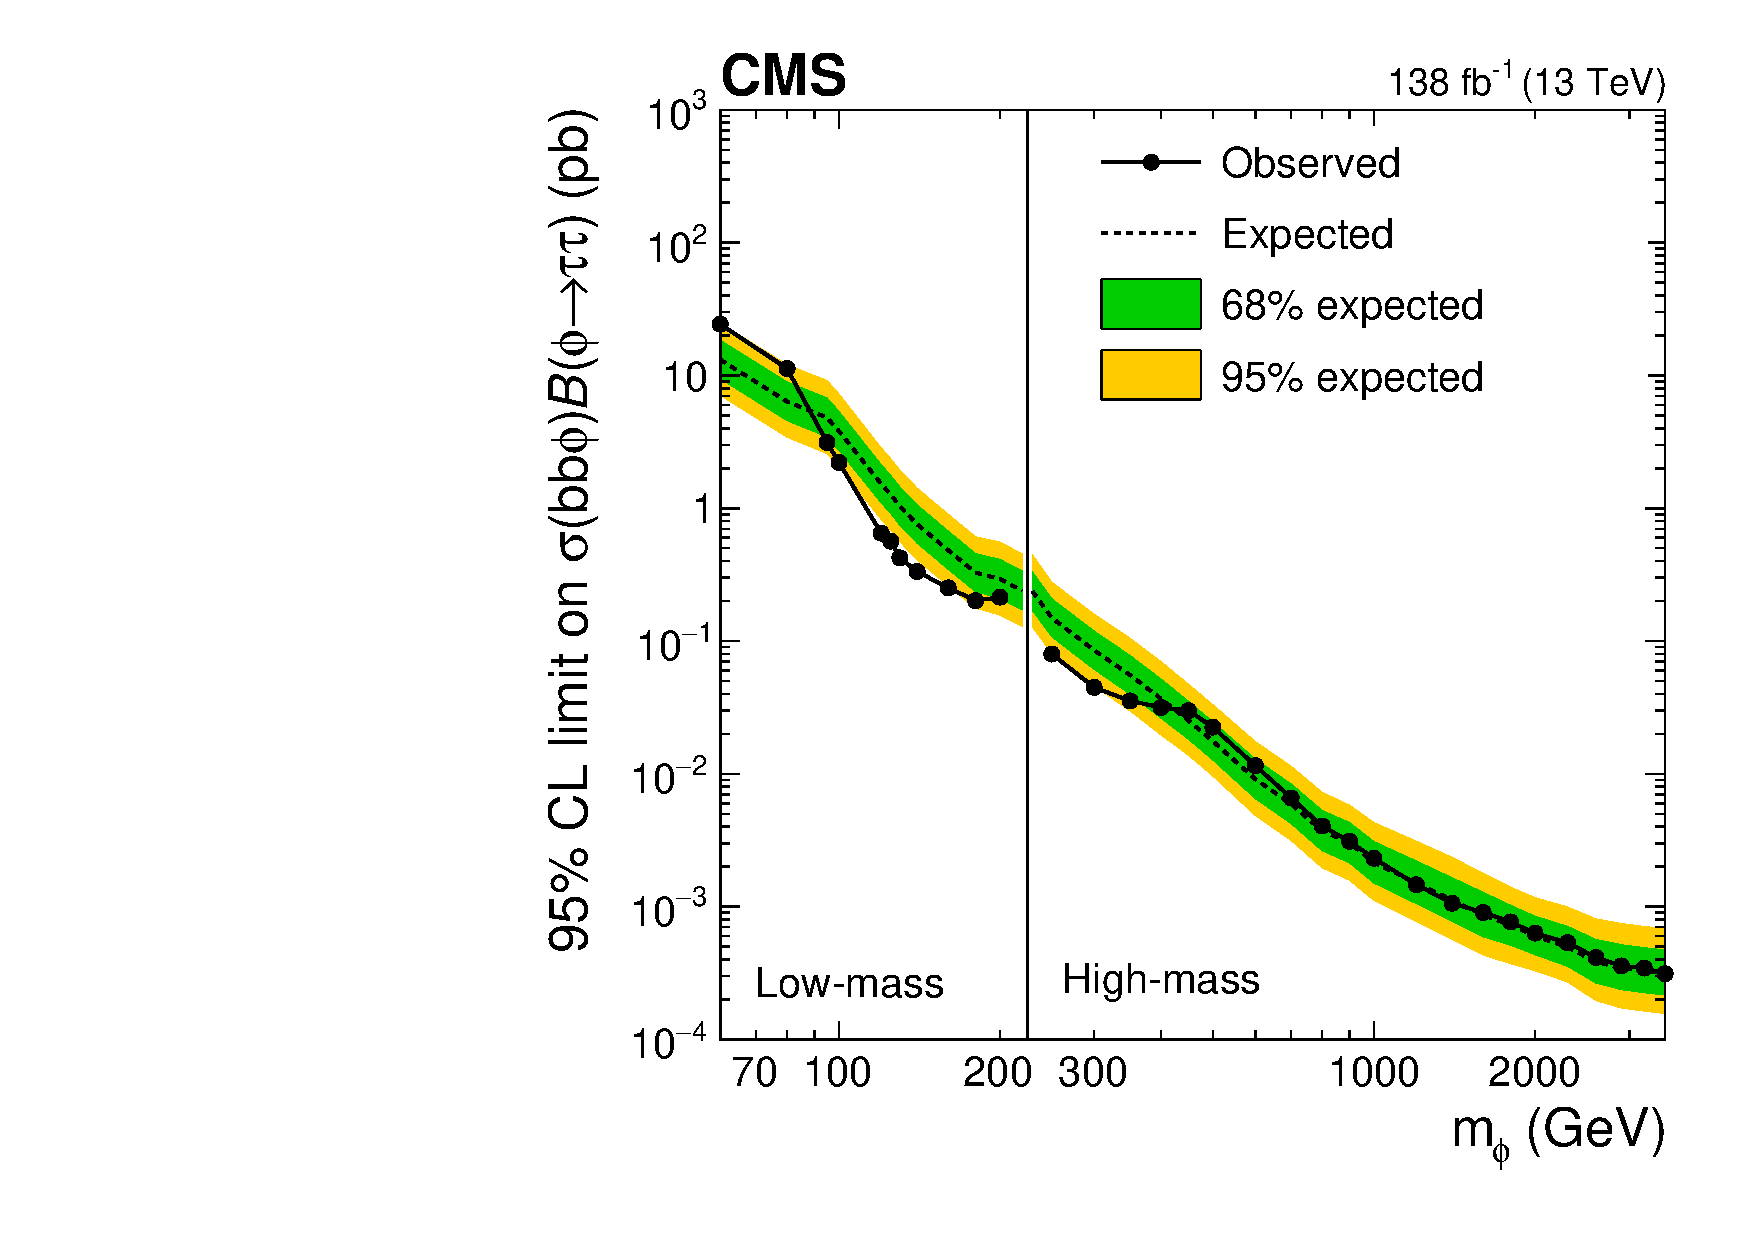
\includegraphics[width=0.65\textwidth]{Figures/model_independent_limit_bbH.pdf}}
\caption[Plots of the model-independent limits on the cross-sections of gluon fusion and b-associated production multiplied by the $\tau\tau$ branching fraction.]{Expected (dashed line) and observed (solid line and dots) 95\% CL upper limits on the product of the cross-sections and branching fraction for the decay into $\tau$ leptons for gg$\phi$ (a) and bb$\phi$ (b) production in a mass range of 60 $\leq m_{\phi} \leq$ 3500 GeV.  The dark green and bright yellow bands indicate the central 68\% and 95\% intervals for the expected exclusion limit~\cite{CMS:2022rbd}.}
\label{fig:model_independent_limits}
\end{figure}

95\% \ac{CL} expected limits are drawn on the fit to each di-$\tau$ decay channel individually and are shown in Figure~\ref{fig:model_independent_limits_by_channel}.
This gives a measure of the sensitivity of each channel.
In the high-mass optimisation categories, the combined limit is heavily dominated by the $\tauhtauh$ channel.
This is mostly driven by the branching fractions, as all channels in this mass range have similar signal separation ability.
In the high-mass optimisation categories, the combined limit is more a contribution of all channels. 
In the $\tauhtauh$ channel in this region, the \ac{QCD} multijet background is the largest fraction of any non $Z\rightarrow\tau\tau$ backgrounds in all channels and so the limit for this channel is weakened and the other channels contribute to the combined limit more.
The high double-$\tau_h$ trigger $\pT$ thresholds (chosen because of the \ac{QCD} multijet background) also lowers the signal acceptance in the $\tauhtauh$ channel. \\

\begin{figure}[!hbtp]
\centering
    \subfloat[]{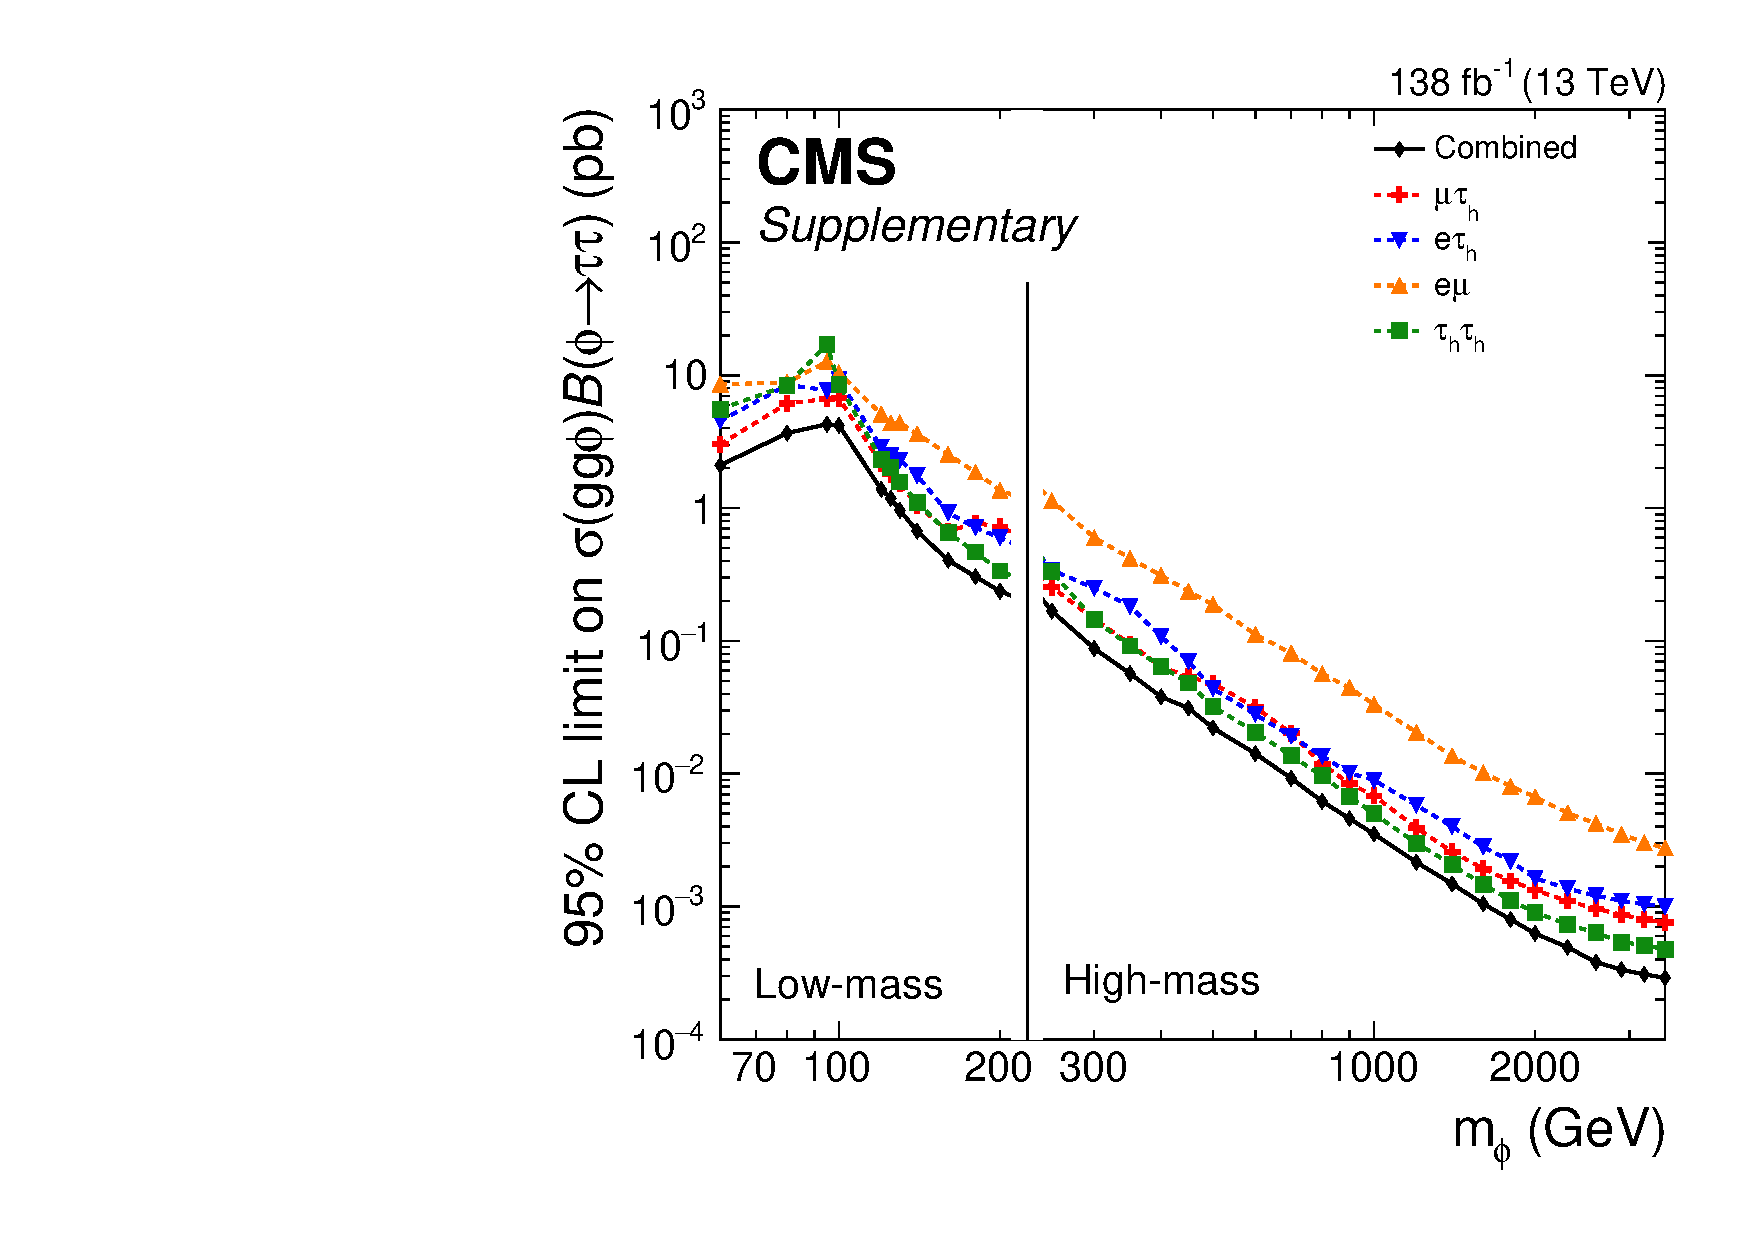
\includegraphics[width=0.5\textwidth]{Figures/limit_comparison_mssm_ggphi.pdf}}
    \subfloat[]{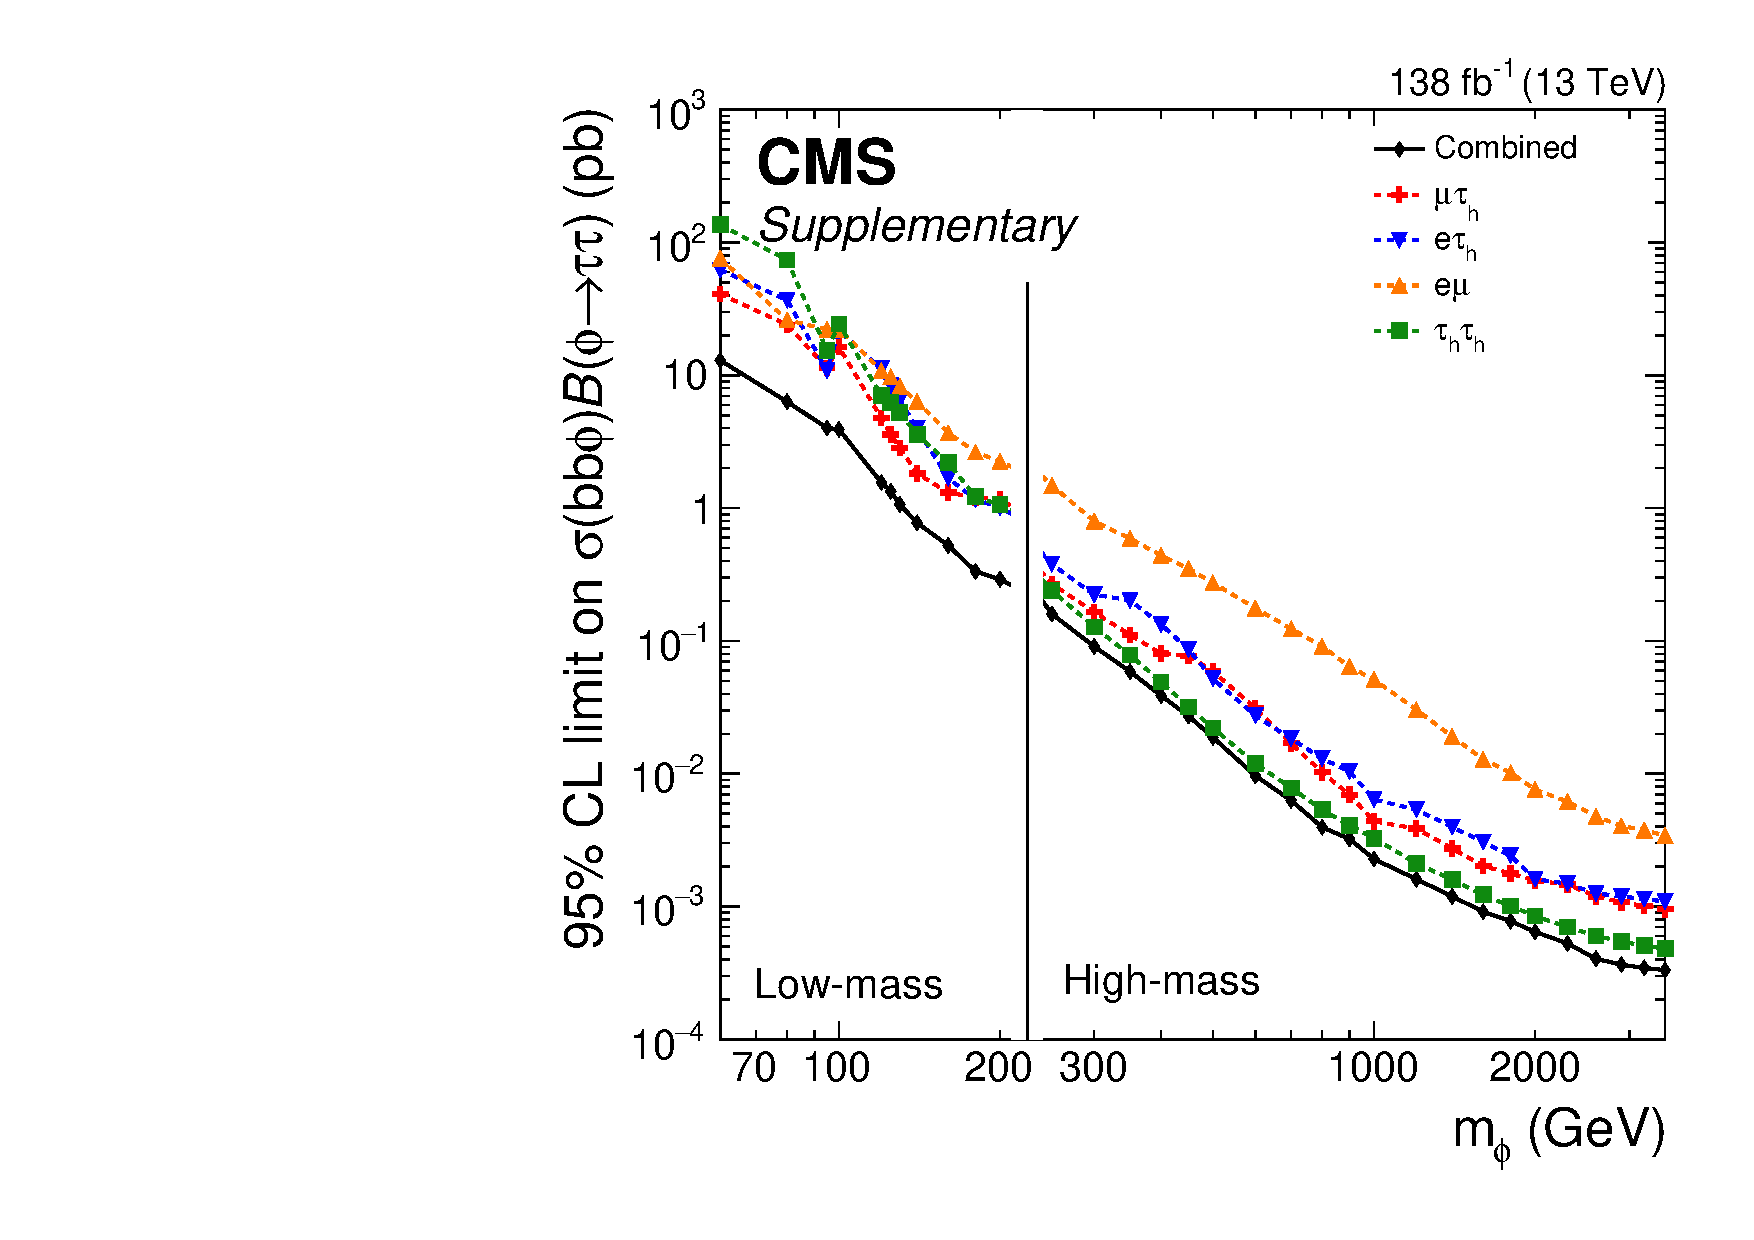
\includegraphics[width=0.5\textwidth]{Figures/limit_comparison_mssm_bbphi.pdf}}
\caption[Plots of the expected model-independent limits split by the $\tau\tau$ decay channels.]{Comparison of the expected 95\% CL upper limits on the product of the cross-sections and branching fraction for the decay into $\tau$ leptons for gg$\phi$ (a) and bb$\phi$ (b) production, split by the $\tau\tau$ decay products fit individually.}
\label{fig:model_independent_limits_by_channel}
\end{figure}

A comparison of the limits is also made with the ATLAS experiment and in particular the results presented in Reference~\cite{ATLAS:2020zms}.
This ATLAS search looks for the same signal but over a smaller mass range, from 200 GeV to 2.5 TeV.
Plots showing the comparison of the expected and observed limits for gg$\phi$ and bb$\phi$ are shown in Figure~\ref{fig:model_independent_limits_ATLAS}.
The expected limits from the \ac{CMS} and ATLAS results are roughly compatible over the shared mass range, except at high mass where the extra statistics from the embedded genuine di-$\tau$ samples compared to \ac{MC} allow for lower background uncertainties and hence a stronger limit.
The ATLAS result observed no excess of events compatible with a gg$\phi$ signal at 1.2 TeV, in fact, a small deficit was observed.
Also, ATLAS observed local excesses at 400 GeV of 2.2$\sigma$ for gg$\phi$ and 2.7$\sigma$ for bb$\phi$.
None of these excesses are consistent between the ATLAS and \ac{CMS} results.
The ATLAS search does not stretch to the mass of the low mass \ac{CMS} excess and so cannot be used as a cross-check for this.

\begin{figure}[!hbtp]
\centering
    \subfloat[]{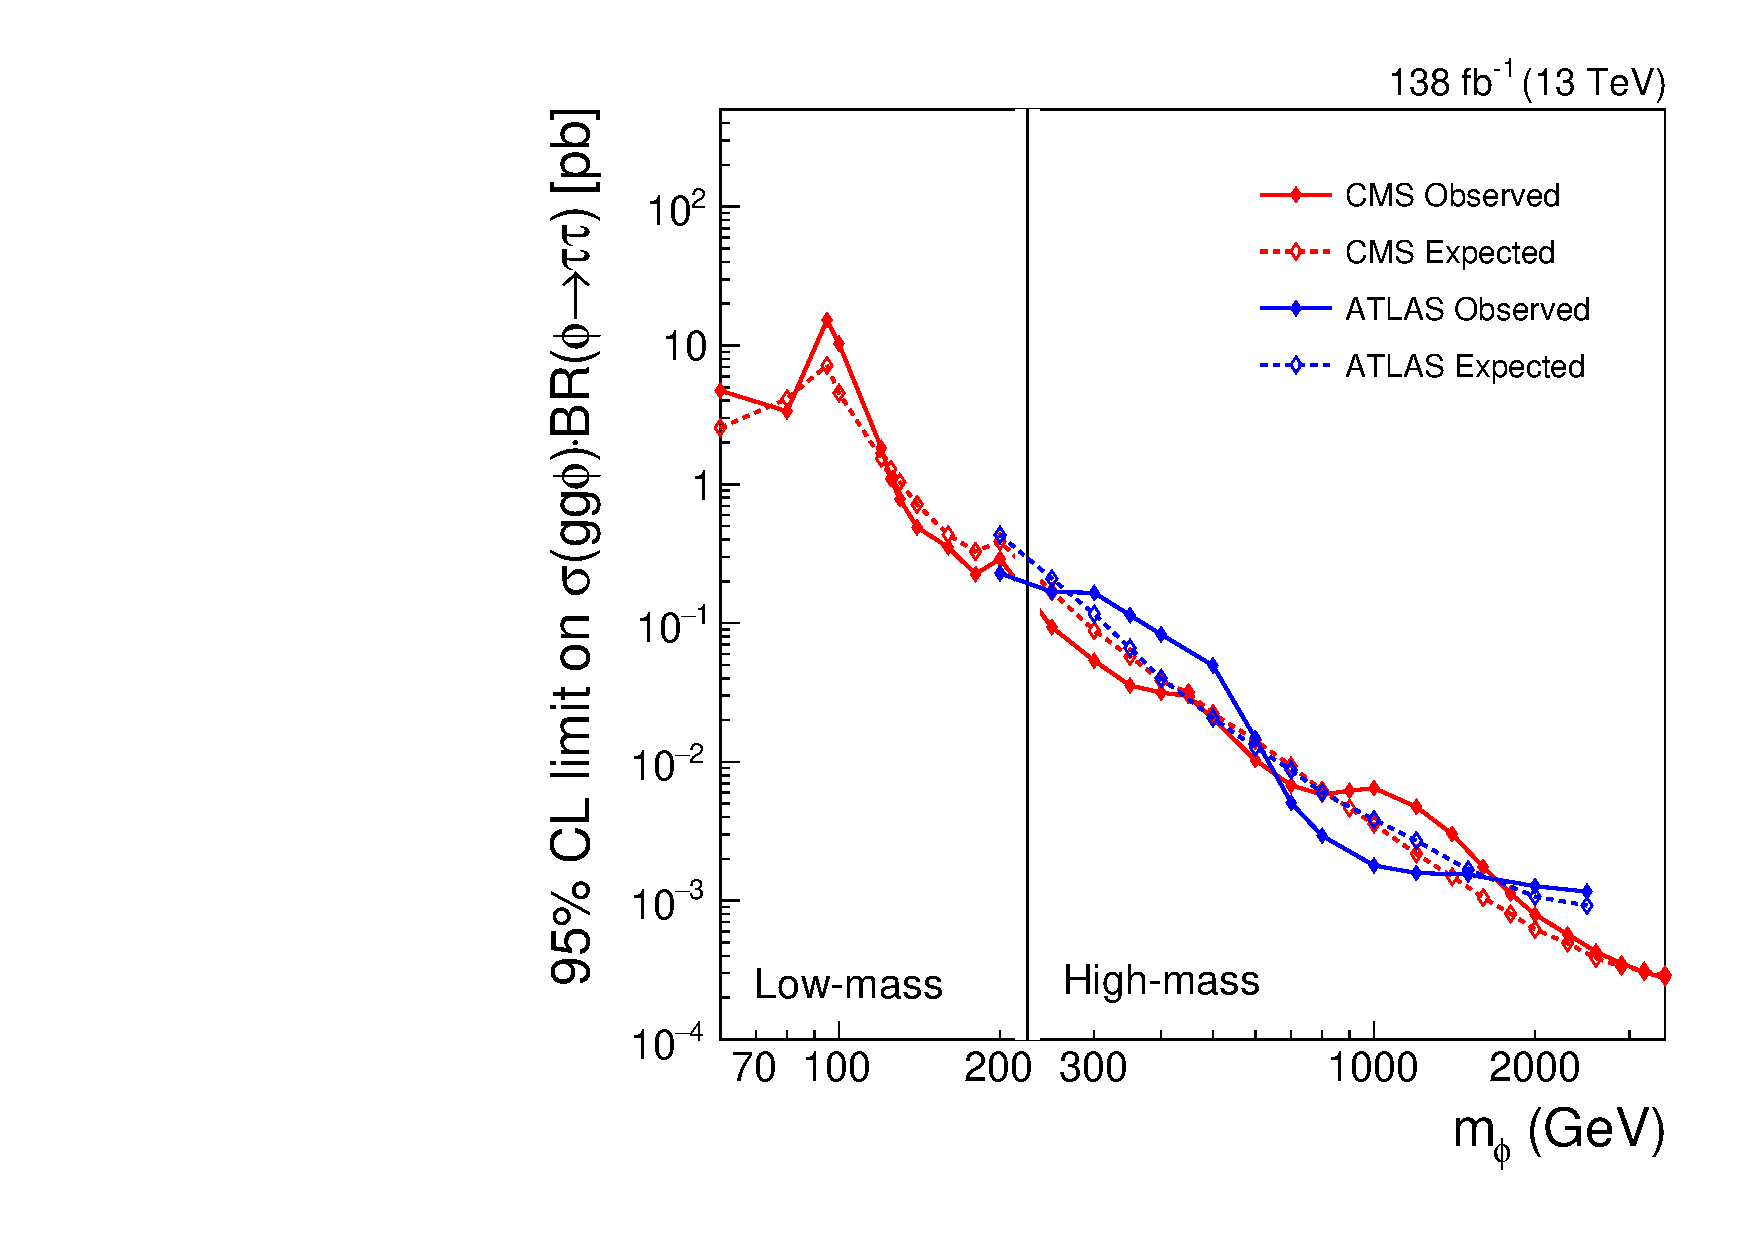
\includegraphics[width=0.5\textwidth]{Figures/limit_comparison_gg_ATLAS.pdf}}
    \subfloat[]{\includegraphics[width=0.5\textwidth]{Figures/limit_comparison_bb_ATLAS.pdf}}
\caption[Plots of the comparison of the model-independent limits between CMS and ATLAS.]{Comparison of the expected 95\% CL upper limits on the product of the cross-sections and branching fraction for the decay into $\tau$ leptons for gg$\phi$ (a) and bb$\phi$ (b) production, split by the CMS result detailed in this thesis and the ATLAS result from Reference~\cite{ATLAS:2020zms}.}
\label{fig:model_independent_limits_ATLAS}
\end{figure}

\subsection{Significance and compatibility}
\label{sec:sig_and_compat}

The $p$-values and significances at each model-independent signal hypothesis are calculated as described in Section~\ref{sec:sig_ext} and shown in Figure~\ref{fig:significance}.
Identical to the model-independent limits, the gg$\phi$ or bb$\phi$ process is allowed to float freely if not the parameter of interest.
The excesses for the gg$\phi$ process peak at 100 GeV and 1.2 TeV and quantify to a local (global) significance of 3.1$\sigma$ (2.7$\sigma$) and 2.8$\sigma$ (2.2$\sigma$) respectively.
There are also excesses at neighbouring mass points (particularly at high mass), however, this is consistent with the mass resolution of the fitted templates for the central values.
No deviations beyond 2$\sigma$ are observed for bb$\phi$ production. \\

\begin{figure}[!hbtp]
\centering
    \subfloat[]{\includegraphics[width=0.5\textwidth]{Figures/significance_plot_ggH.pdf}}
    \subfloat[]{\includegraphics[width=0.5\textwidth]{Figures/significance_plot_bbH.pdf}}
\caption[Plots of the local $p$-value and significance for gluon fusion and b-associated production.]{Local $p$-value and significance of a gg$\phi$ (a) and bb$\phi$ (b) signal as a function of $m_{\phi}$~\cite{CMS:2022rbd}.}
\label{fig:significance}
\end{figure}

As many different decay channels and categories are used to extract these significances, the signal strength is studied in each channel and category.
This is done via compatibility fits as described in Section~\ref{sec:sig_ext}, where the signal strength parameter in each channel/category is decoupled.
No statistically significant differences are observed in the best-fit signal strength in any decay channel or category fit and $p$-values between each channel or category fit are always above 0.05.
Figure~\ref{fig:low_mass_compatibility} shows the results of the compatibility fits in the low-mass optimisation categories split by di-$\tau$ decay channels and the $\pT$ bins fit. 
Figure~\ref{fig:high_mass_compatibility} shows the compatibility fits in the high-mass optimisation categories split by di-$\tau$ decay channels.
The low-mass signal strengths are no more dominant in any $\pT$ region than another.
In both low- and high-mass cases, the signal strengths are consistent across di-$\tau$ decay channels.
There is a small shift in the high mass $\emu$ categories to a negative signal strength, these categories have little to no sensitivity to this signal in comparison to others and a small deficit is observed in data, resulting in fits for a negative signal strength with a large uncertainty. 


\begin{figure}[!hbtp]
\centering
    \subfloat[]{\includegraphics[width=0.5\textwidth]{Figures/ChannelCompatibilityCheck_FitResults_mH100_channel.pdf}}
    \subfloat[]{\includegraphics[width=0.5\textwidth]{Figures/ChannelCompatibilityCheck_FitResults_mH100_cat.pdf}}
\caption[Plots of the compatibility of the 100 GeV excess across the channels and categories.]{Compatibility plots of the 100 GeV excess split into analysis channels (a) and categories (b). In each case, the fitted signal strength is decoupled in the bin shown on the plot~\cite{CMS:2022rbd}.}
\label{fig:low_mass_compatibility}
\end{figure}

\begin{figure}[!hbtp]
\centering
    \includegraphics[width=0.5\textwidth]{Figures/ccc_fit_result_mH1200_per-channel.pdf}
\caption[Plots of the compatibility of the 1.2 TeV excess across the channels.]{Compatibility plots of the 1.2 TeV excess split by analysis channels. In each case, the fitted signal strength is decoupled in each channel~\cite{CMS:2022rbd}.}
\label{fig:high_mass_compatibility}
\end{figure}

\subsection{2D likelihood scans}

As the model-independent search looks for two signal modes at each mass point, the results for both processes happening simultaneously are studied.
This is done in the form of two-dimensional likelihood scans.
The best-fit cross-section times branching fractions of each process and the 95\% and 68\% confidence intervals are shown for a number of different mass scenarios in Figure~\ref{fig:2d_likelihood_scans}.
The \ac{SM} prediction in all plots is at (0,0).
These results highlight how the excesses at 100 GeV and 1.2 TeV are dominated in the phase space in which gg$\phi$ and not bb$\phi$ signals are allowed.
In the 60 GeV example, there are smaller deviations in both gg$\phi$ and bb$\phi$ and the SM background is again over 2$\sigma$ away.
Otherwise, signal strengths are completely compatible with the background expectation.


\begin{figure}[!hbtp]
\centering
    \subfloat[]{\includegraphics[width=0.33\textwidth]{Figures/2d_lkld_60.pdf}}
    \subfloat[]{\includegraphics[width=0.33\textwidth]{Figures/2d_lkld_100.pdf}}
    \subfloat[]{\includegraphics[width=0.33\textwidth]{Figures/2d_lkld_125.pdf}} \\
    \subfloat[]{\includegraphics[width=0.33\textwidth]{Figures/2d_lkld_160.pdf}}
    \subfloat[]{\includegraphics[width=0.33\textwidth]{Figures/2d_lkld_250.pdf}}
    \subfloat[]{\includegraphics[width=0.33\textwidth]{Figures/2d_lkld_500.pdf}} \\
    \subfloat[]{\includegraphics[width=0.33\textwidth]{Figures/2d_lkld_1000.pdf}}
    \subfloat[]{\includegraphics[width=0.33\textwidth]{Figures/2d_lkld_1200.pdf}}
    \subfloat[]{\includegraphics[width=0.33\textwidth]{Figures/2d_lkld_3500.pdf}}
\caption[Plots of the maximum likelihood scans for the model-independent search.]{Maximum likelihood scans, including 68\% and 95\% CL contours obtained from the signal likelihood for the model-independent search. The scans are shown for$m_{\phi}$ values of 60 (a), 100 (b), 125 (c), 160 (d), 250 (e), 500 (f), 1000 (g), 1200 (h) and 3500 (i) GeV~\cite{CMS:2022rbd}.}
\label{fig:2d_likelihood_scans}
\end{figure}

\section{Model-dependent limits}

The exclusion contours for two benchmark scenarios of the \ac{MSSM}, $M_{h}^{125}$ and $M_{h,EFT}^{125}$, are presented in Figure~\ref{fig:mssm_limits}. 
The red hatched regions denote areas where $m_{h}$ is inconsistent with the observed \ac{SM} Higgs boson mass within a ${\pm}3$ GeV boundary. 
For low values of $\tan\beta$, higher values of the additional SUSY particle masses, denoted as $m_{\text{SUSY}}$, are needed to explain a mass of approximately $125$ GeV for the Higgs boson. 
In the $M_{h}^{125}$ scenario, $m_{\text{SUSY}}$ is fixed, and the predicted value of $m_{h}$ is below $122$ GeV. 
In contrast, the $M_{h,EFT}^{125}$ scenario adjusts $m_{\text{SUSY}}$ to satisfy the required value of $m_{h}$ for each point in $m_{A}$ and $\tan\beta$ individually, accounting for the logarithmic corrections associated with the large values of $m_{\text{SUSY}}$ using an effective field theory approach. 
The red hatched region in Figure~\ref{fig:mssm_limits}b indicates that the required values of $m_{\text{SUSY}}$ exceed the GUT scale at very low values of $m_{A}$ in this scenario. 
The Higgs boson masses, mixing angle $\alpha$, and effective Yukawa couplings were calculated using \textsc{FeynHiggs}, and branching fractions for the decay into $\tau$ leptons and other final states were obtained from a combination of the \textsc{FeynHiggs} and \textsc{HDECAY}, following the prescriptions in References~\cite{LHCHiggsCrossSectionWorkingGroup:2013rie,deFlorian:2016spz,Denner:2011mq}, for the scenarios described in Reference~\cite{Bagnaschi:2791954}. \\

For the $M_{h,EFT}^{125}$ scenario, the sensitivity sharply drops at $m_{A}=2m_{t}$ due to a drop in the branching fractions for the decay of A and H into $\tau$ leptons, when the A and H decay into two on-shell t quarks becomes kinematically accessible. 
Both scenarios are excluded at 95\% CL for $m_{A}\lesssim350$ GeV. 
For $m_{A}\lesssim250$ GeV, most of the ggH/A events do not enter the no b tag categories due to the $m_{\tau\tau}>250$ GeV requirement. 
In this parameter space, the sensitivity to the \ac{MSSM} is driven by the measurements of the observed Higgs boson, even though H and A still contribute to the categories here. 
The sensitivity to the H and A enters mainly via the bb$\phi$ signal in the b tag categories, especially for increasing values of $\tan\beta$. \\

Other \ac{MSSM} scenarios are tested and detailed in Reference~\cite{CMS:2022rbd}.
One scenario of note is the $M_{H}^{125}$ scenario, which is the equivalent scenario to the $M_{h}^{125}$ but with the observed Higgs boson being the heavier \ac{CP}-even Higgs boson.
Despite the local excess at a resonant mass of 100 GeV, this scenario is entirely excluded by the search. 
This is mostly due to the sensitivity of the b tag categories to b-associated production.
The local excess observed at 1.2 TeV is hard to rectify within these \ac{MSSM} benchmark scenarios.
The lack of any excess in the b tag categories strictly constrains the b-associated production cross-section times the branching fractions.
It is not possible within these scenarios to predict the excess of gluon fusion events within the constraints placed on b-associated production. \\

\begin{figure}[!hbtp]
\centering
    \subfloat[]{\includegraphics[width=0.65\textwidth]{Figures/model-dependent_limit_mh125.pdf}} \\
    \subfloat[]{\includegraphics[width=0.65\textwidth]{Figures/model-dependent_limit_mh125EFT.pdf}}
\caption[Plots of the model-dependent limits in MSSM benchamrk scenarios.]{Expected and observed 95\% CL exclusion contours in the MSSM $M_{h}^{125}$ (a) and $M_{h,EFT}^{125}$ (b) scenarios. The exclusion limit only on background expectation is shown as a dashed black line, the dark and bright grey bands show the 68\% and 95\% intervals of the expected exclusion and the observed exclusion contour is shown by the blue area. The parameter space where $m_{h}$ deviates by more than $\pm$3  GeV from the observed SM Higgs boson mass is shown by a red-hatched area.~\cite{CMS:2022rbd}
}
\label{fig:mssm_limits}
\end{figure}

Upper limits of 95\% \ac{CL} for VLQ BM 1 and 2 are shown in Figure~\ref{fig:vlq_limits}. 
These are drawn with respect to the leptoquark mass ($m_{U}$) and coupling ($g_{U}$).
The limit on $g_{U}$ decreases as $m_{U}$ increases, with values of $g_U$ ranging from 1.3 to 5.2 in VLQ BM 1 and 0.8 to 3.2 in VLQ BM 2. 
VLQ BM 2 has stronger exclusion limits than VLQ BM 1 due to additional right-handed couplings of the leptoquark with a b quark and a $\tau$ lepton. \\

\begin{figure}[!hbtp]
\centering
    \subfloat[]{\includegraphics[width=0.65\textwidth]{Figures/vlq_bm_1.pdf}} \\
    \subfloat[]{\includegraphics[width=0.65\textwidth]{Figures/vlq_bm_2.pdf}}
\caption[Plots of the model-dependent limits in the vector leptoquark phase space.]{Expected and observed 95\% CL upper limits on $g_U$ in the VLQ BM 1 (a) and 2 (b) scenarios, in a mass range of $1<m_{U}<5$ TeV.  The exclusion limit only on that background expectation is shown as a dashed black line, the dark and bright grey bands show the 68\% and 95\% intervals of the expected exclusion and the observed exclusion contour is shown by the blue area. The 95\% confidence interval for the preferred region from the global fit presented in Reference~\cite{Cornella:2021sby} is also shown by the green shaded area~\cite{CMS:2022rbd}.}
\label{fig:vlq_limits}
\end{figure}

The observed limits fall within the central 95\% intervals of the expected limits when no signal is present. 
The expected limits are also within the 95\% confidence interval of the best fit results reported by Reference~\cite{Cornella:2021sby} and described in Section~\ref{sec:b_anomalies}.
This indicates that the search is capable of detecting a part of the parameter space that can explain the anomalies observed in B physics and since no significant excess was observed in this search, new constraints are placed on the vector leptoquark phase space.
Similarly to the \ac{MSSM} scenarios, the local excess at 1.2 TeV is not consistent with a VLQ BM 1 or 2 vector leptoquark.
Again this is due to the lack of signal in the b tag categories, where the reduction in backgrounds makes the t-channel signal with initial state radiation the dominant search option.


